\documentclass[12pt,a4paper]{scrartcl}

%========================================================================================
%SPRACHE

\usepackage[ngerman]{babel} 
\usepackage[T1]{fontenc} 				% richtige Silbentrennung
\usepackage[utf8]{inputenc}    % Umlaute etc.!!! BENUTZEN!!!!
\usepackage{float} % alles möglichen Sachen mit [h] an die richtige Stelle zwingen
%\usepackage{rotating} % tabellen rotieren
%\usepackage{supertabular} % schraege tabellen etc
%\usepackage{pdfpages}     % pdfs einbinden


\usepackage{setspace}

\usepackage[]{natbib}

%========================================================================================
%DARSTELLUNG

\usepackage[small,compact]{titlesec} 		% Verkleinerung von Section-Ueberschriften
\usepackage{graphicx}				  	% Einbinden von Graphiken .ps, .pdf, .png

\usepackage{amsmath}					% mathematische Symbole
%\usepackage {ulem} 						%\emph{Text}: Text wird unterstrichen
\setlength{\parindent}{0pt}				% Zeile nach Absatz einruecken 1pt oder nicht 0pt.

%========================================================================================
%FARBEN

\usepackage[usenames,dvipsnames]{color}	

									%Apricot 	Aquamarine 	Bittersweet 	Black
									%Blue 	BlueGreen 	BlueViolet 	BrickRed
									%Brown 	BurntOrange 	CadetBlue 	CarnationPink
									%Cerulean 	CornflowerBlue 	Cyan 	Dandelion
									%DarkOrchid 	Emerald 	ForestGreen 	Fuchsia
									%Goldenrod 	Gray 	Green 	GreenYellow
									%JungleGreen 	Lavender 	LimeGreen 	Magenta
									%Mahogany 	Maroon 	Melon 	MidnightBlue
									%Mulberry 	NavyBlue 	OliveGreen 	Orange
									%OrangeRed 	Orchid 	Peach 	Periwinkle
									%PineGreen 	Plum 	ProcessBlue 	Purple
									%RawSienna 	Red 	RedOrange 	RedViolet
									%Rhodamine 	RoyalBlue 	RoyalPurple 	RubineRed
									%Salmon 	SeaGreen 	Sepia 	SkyBlue
									%SpringGreen 	Tan 	TealBlue 	Thistle
									%Turquoise 	Violet 	VioletRed 	White
									%WildStrawberry 	Yellow 	YellowGreen 	YellowOrange
									
									% verwenden mit: 
									% \pagecolor{declared-color}
									% {\color{declared-color} text}
									% \colorbox{declared-color1}{\color{declared-color2} text}
									%========================================================================================
%Zur Einbindung von Programmiertexten mit:
				% \begin{lstlisting}
				%put your code here
				%\end{lstlisting}
				
\usepackage{listings}
\lstset{ %
language=C,                			% the language of the code
basicstyle=\footnotesize,       			% the size of the fonts that are used for the code
numbers=left,                   				% where to put the line-numbers
numberstyle=\footnotesize,      			% the size of the fonts that are used for the line-numbers
stepnumber=1,                   				% the step between two line-numbers. If it's 1, each line 
                                					% will be numbered			
commentstyle=\color{PineGreen},					
numbersep=-7pt,                  			% how far the line-numbers are from the code
backgroundcolor=\color{white},  		% choose the background color. You must add \usepackage{color}
showspaces=false,               			% show spaces adding particular underscores
showstringspaces=false,        		 	% underline spaces within strings
showtabs=false,                 				% show tabs within strings adding particular underscores
frame=single,                   				% adds a frame around the code
tabsize=2,                      				% sets default tabsize to 2 spaces
captionpos=b,                   				% sets the caption-position to bottom
breaklines=true,                				% sets automatic line breaking
breakatwhitespace=false,        			% sets if automatic breaks should only happen at whitespace
title=\lstname,                 				% show the filename of files included with \lstinputlisting;
                                					% also try caption instead of title
}
%========================================================================================


%LOAD FANCYHDR fuer Kopf- und Fu{\ss}zeilen
%\usepackage{fancyhdr}					% Paket laden	f\"ur einfache Handhabung von Kopf-und Fu{\ss}zeile
%\fancyhf{}								% alle Kopf- und Fu{\ss}zeilen bereinigen
%\pagestyle{fancy}						% Deklariere Seitenstil
%----------------------------------------------------------------------------------------------------------------------------------------------------------
% Angaben fuer Kopf-und Fu{\ss}zeilen links[L] und rechts[R]		
%\fancyhead[L]{{\textbf{Entwicklung eines Schwingungsmesssystems für ein Radar}}}
%\fancyfoot[C]{\thepage} 					% Seitennummer unten mittig

\usepackage[headsepline,plainheadsepline]{scrpage2}
\pagestyle{scrheadings}
\ihead[\rightmark]{\rightmark} \chead[]{}
\ohead[\pagemark]{\pagemark} \cfoot[]{}

\automark{section}
\renewcommand{\sectionmark}[1]{\markright{\ #1}}


\usepackage[small, nooneline, bf]{caption}

\addto\captionsngerman{
\renewcommand{\figurename}{Abb.}
\renewcommand{\tablename}{Tab.}
}

\usepackage{booktabs}
\usepackage{subfigure}



%==========================================================================================

\begin{document}

\title {Entwicklung eines Schwingungsmesssystems für ein Radar}
\author{Sebastian Beyer}
\maketitle
\thispagestyle{empty}
\newpage

\tableofcontents
\thispagestyle{empty}
\newpage




\section{Kurzfassung}

\newpage

\section{Motivation}

Mit einem Dopplerradar lassen sich vulkanische Eruptionen quantitativ erfassen und auswerten. In vielen Studien haben diese Messungen bereits neue Erkenntnisse über die dahinter liegenden Prozesse gebracht. 

Ursprünglich in der Metrologie zur Regenmessung eingesetzt, ermöglichen Dopplerradargeräte Geschwindigkeiten von Partikeln in der Eruptionssäule zu ermitteln. Ein Radar der Firma Metek ist in Abbildung \ref{radar} zu sehen.

Über eine Satellitenantenne wird ein Radarstrahl mit der Wellenlänge von 1.25cm gebündelt und auf die Eruptionssäule gerichtet.
Aus der zurückgestreuten Energie ermittelt das Radar dann eine Geschwindigkeitsverteilung der Streukörper. 

Ein Radar kann entweder klassisch mit gepulsten Signalen oder mit einer zeitlich konstanten Sendeleistung arbeiten.
Im ersten Fall ergibt sich die Entfernung eines Objektes durch die Laufzeit eines abgestrahlten Pulses. 
Wir arbeiten jedoch mit einem konstanten Signal und bestimmen die Entfernung über eine Frequenzmodulation. Dieses Verfahren nennt man \textit{Frequency Modulated Continous Wave}. Die zeitliche Auflösung ist zwar nicht so hoch wie bei einem gepulsten Radar, aber dafür ist der Energieverbrauch deutlich geringer.


\begin{figure}[htb]
\centering
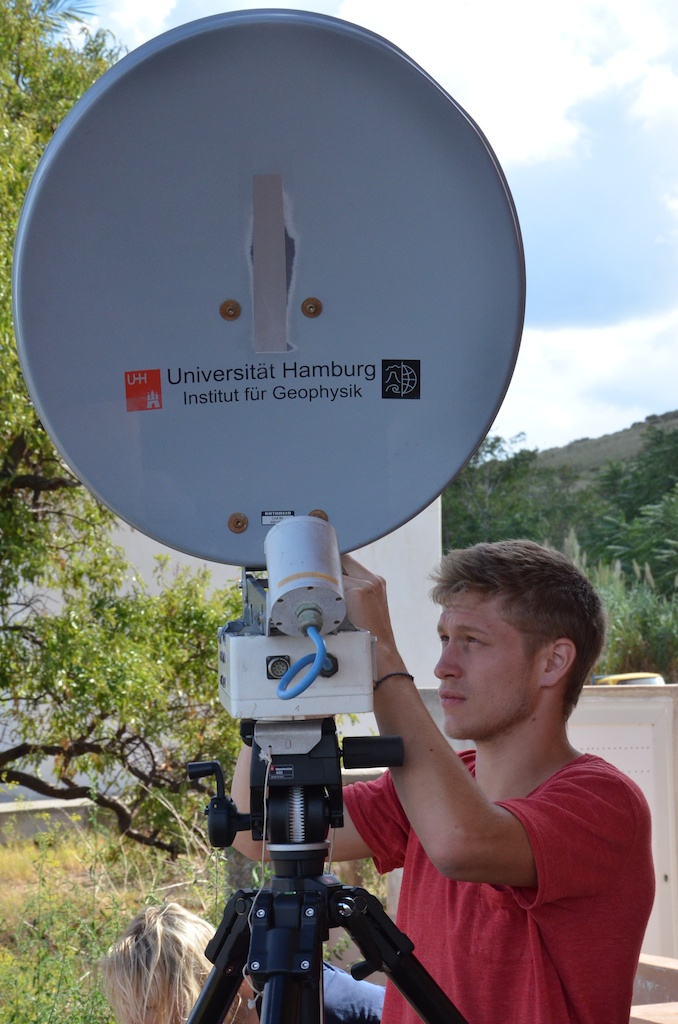
\includegraphics[scale=.3]{hardwareimages/radar.jpg}
\caption{Aufbau des Metek Dopplerradars auf Stromboli mit Martin Vögele}
\label{radar}
\end{figure}

Das Funktionsprinzip des Doppler Radars beruht auf dem Frequenzunterschied zwischen gesendetem und empfangenen Signal. Dieser Unterschied ist direkt proportional zur Geschwindigkeit eines Objekts, welches sich entlang des Radarstrahls bewegt. Eine genaue Beschreibung des Prinzips ist in \citep{Hort:2003fk} zu finden. \\

Sehr langsame Bewegungen rufen einen zu geringen Frequenzunterschied hervor und sind aus diesem Grund nicht auflösbar. Betrachtet man allerdings die Phasenverschiebung des Signals, so lässt sich aus diesen Informationen auch die langsame Änderung der Entfernung eines Objekts sehr genau bestimmen. 
Mit dieser sogenannten \textit{Phasenmessung} können zum Beispiel relativ langsam ablaufende Deformationsprozesse von Vulkanen im Millimeterbereich untersucht werden.

\begin{figure}[htb]
\centering
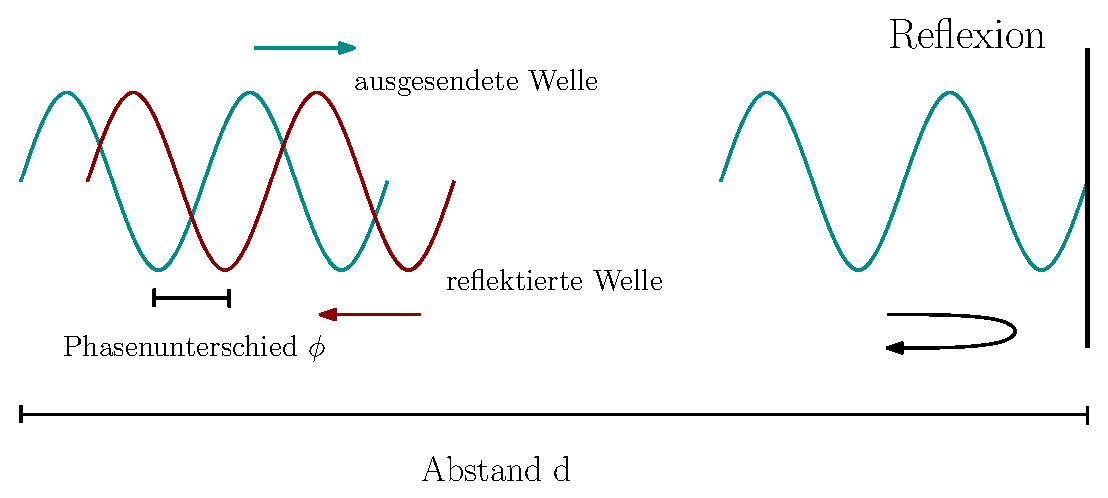
\includegraphics[scale=.8]{phasenmessung.eps}
\caption{Prinzip der Phasenmessung. Zum besseren Verständnis dargestellt für ein gepulstes Radar.}
\label{phasenmessung}
\end{figure}

Das Funktionsprinzip ist ins Abbildung \ref{phasenmessung} zu sehen. Aus Gründen der Darstellbarkeit und des besseren Verständnisses verwende zur Erklärung ein gepulstes Radar.

Das empfangene Signal wird mit dem ausgehenden Verglichen. Dabei tritt ein Phasenunterschied $\phi$ auf, der vom Abstand $d$ zwischen Radar und Reflektor abhängt. Jede Änderung im Phasenunterschied bedeutet eine Änderung des Abstandes. Zu beachten ist, dass dieses Verfahren keinen absoluten Abstand liefert, sondern immer nur eine relative Änderung zu einem gewählten Referenzpunkt.\\

Mit dieser Vorgehensweise konnten am Santiaguito Vulkan in Guatemala 2007 bereits Hebungen und Senkungen von mehreren Zentimetern Höhe wenige Sekunden vor und nach einer Eruption festgestgestellt werden \citep{Scharff:2007uq}. \\

Bei diesen Messverfahren wird stets davon augegangen, dass das Radar fest auf einem Stativ fixiert ist und sich nicht bewegt. Sämtliche gemessene Bewegung wird als Bewegung der beobachteten Objekte gewertet. 
In der Praxis kann es allerdings vorkommen, dass sich das Radar aufgrund von Wind, Erschütterungen oder Deformationen des Untergrunds sehr wohl bewegt und in Schwingung gerät. Mit einer alleinigen Abstandsmessung lassen sich diese Bewegungen des Messgerätes nicht von denen des Messobjektes unterscheiden.\\

Aus diesem Grund entwickle ich in dieser Arbeit ein Schwingungsmessystem mit einem dreiachsigen Beschleunigungssensor und teste dieses anhand einiger Experimente.

Das Ziel ist es, zusätzlich zu den Radardaten Beschleunigungen aufzuzeichnen und aus diesen die Bewegung des Radarsystems zu berechnen. Damit ließen sich die Radardaten korrigieren und man könnte mit größerer Sicherheit sagen, ob eine Beobachtete Bewegung in den Radaraufzeichnungen auf eine Bewegung des Messobjektes oder auf eine Bewegung des Radars selber zurückzuführen ist.\\

{\color{red}(Vorgehen und Aufbau der Arbeit beschreiben??)}

\newpage

\section{Beschleunigungssensoren}
\onehalfspacing
Beschleunigungssensoren messen die Beschleunigung, die auf ein System wirkt, indem sie die auf eine Testmasse wirkenden Kräfte bestimmen. Nach Newton  Die auf einen Körper wirkende Beschleunigung setzt sich aus der Gravitation und Trägheitskräften zusammen. Isoliert man die Trägheitskräfte, so lässt sich daraus die Translationsbeschleunigung bestimmen. Mithilfe dieser und dem zweiten newtonschen Gesetz lässt sich die Positionsänderung des Systems berechnen: 

\begin{equation}
F = m \cdot a
\end{equation}

Es gibt verschiedene Prinzipien, mit denen Beschleunigung gemessen werden kann. Am gebräuchlichsten ist das der Federwaage.

\begin{figure}[H]
\centering
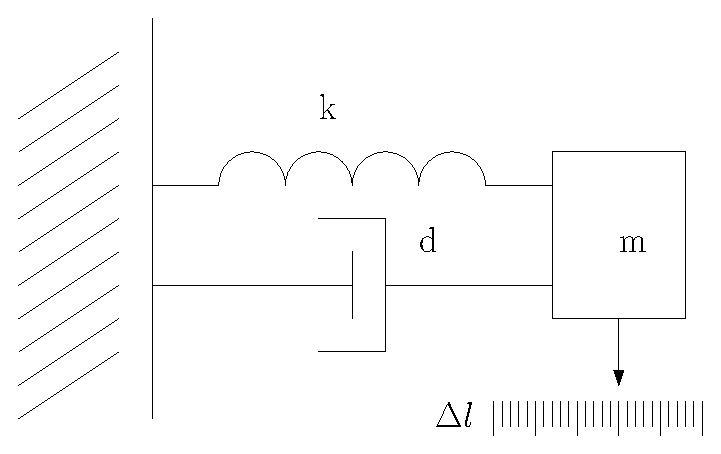
\includegraphics[scale=0.7]{federmasse.eps}
\caption{Masse-Feder-System zur Beschleunigungsmessung. k, d, m und $x$ bezeichnen Federkonstante, Dämpfung, Masse und Auslenkung. nach \citep{Klingbeil:2006qy}.}
\label{federwaage}
\end{figure}

Eine Masse m (auch seismische Masse genannt) ist über eine Feder der Federkonstanten k mit einem festen Bezugspunkt verbunden. Die Auslenkung $x$ ist proportional zur auf die Masse wirkenden Beschleunigung a.
\begin{equation}
a = \frac{k}{m} \cdot x
\end{equation}

Zu beachten ist die Ausrichtung des Sensors: a entspricht immer der Projektion der Beschleunigung auf die Auslenkungsrichtung von m.\\

Das System führt eine gedämpfte harmonische Schwingung aus. Einmal angeregt beginnt es zu schwingen, die Amplitude nimmt dann aber kontinuierlich ab. Die Bewegungsgleichung lautet: (vergleiche auch \citep{Meschede:2001fk})

\begin{equation}
m \ddot x + d \dot x + kx = 0
\end{equation}

Wobei $m$ die Masse, $d$ die Dämpfung und $k$ die Federkonstante ist.
Eine Lösung dieser Differentialgleichung lautet:

\begin{equation}
x(t) = x_0 e^{-\delta t} sin(\omega_d t + \varphi_0) \qquad mit \quad \delta = \frac{d}{2m}
\end{equation}

Die Lösung ist aus zwei elementaren Funktionen zusammengesetzt, wobei die eine den periodischen Anteil ausmacht und die andere den dämpfenden Anteil. Der periodische Anteil lässt ich auch als $x_0 e^{i\omega_d t}$ schreiben, wobei 
\begin{equation}
\omega_d = \sqrt{\omega_0^2 - \delta^2}
\end{equation}
die gedämpfte Eigenfrequenz genannt wird und einen entscheidenden Einfluss auf das Schwingverhalten hat.

Bei kleinem $\delta$ ist die Dämpfung gering und es gilt
\begin{equation}
\omega_d \approx \omega_0
\end{equation}
Dies nennt man den \textit{Schwingungsfall}

Wenn die Dämpfung jedoch so groß wird, dass
\begin{equation}
\delta = \omega_0
\end{equation}
gilt, wird $\omega_d = 0$ und das System kommt in kürzestmöglicher Zeit zur Ruhe. Man spricht vom \textit{aperiodischen Grenzfall}. Dieses Verhalten ist bei Beschleunigungsaufnehmern erwünscht, weil man so die höchste Wiederholfrequenz von Messungen erreicht, ohne dass sich die Anregungen gegenseitig überlagern.\\

Wird $\delta$ noch größer, so wird der Term unter der Wurzel negativ und $\omega_d$ damit imaginär. Aus 
\begin{equation}
e^{i\omega_d t}
\end{equation}
wird
\begin{equation}
e^{-k t}
\end{equation}
und bewirkt eine zusätzliche Dämpfung. Eine Schwingung existiert nicht mehr und das System erreicht seine Ruhelage nach längerer Zeit als beim aperiodischen Grenzfall. Dieses als \textit{Kriechfall} bezeichnete Verhalten ist in den meisten Fällen unerwünscht. \\



Mittlerweile sind Beschleunigungssensoren in den meisten Fällen als MEMS realisiert (\textbf{M}icro \textbf{E}lectro \textbf{M}echanical \textbf{S}ystems). Sehr kleine mechanische Elemente (1-100 Mikrometer) werden zusammen mit elektronischen Schaltungen auf einen Siliziumwafer aufgebracht. Dabei werden Techniken aus der Fabrikation von integrierten Schaltkreisen (ICs) verwendet. So können komplizierte elektromechanische System in winziger Größe und hoher Stückzahl hergestellt werden. Der geringe Preis ist maßgeblich dafür verantwortlich, dass die Sensoren in immer mehr Anwendungen integriert werden (Autos, Smartphones, Quadrokopter…).

Die Beschleunigungsmessung erfolgt also über die Messung der Auslenkung einer Testmasse. Dazu haben sich zwei Verfahren durchgesetzt, die ich im Folgenden kurz erläutern möchte. 

\subsection{Piezoresistive Sensoren}
Piezoresistive Sensoren machen sich den piezoelektrischen Effekt zunutze. In der Feder der Testmasse befinden sich Piezoelemente, welche sich bei Auslenkung verformen und damit ihren Widerstand ändern. Silizium ist ein geeignetes Material, da es sehr empfindlich und linear reagiert und gleichzeitig gut mit der MEMS Technik kombinierbar ist \citep{Kanda:1991gf}.

\subsection{Kapazitative Sensoren}

\begin{figure}[htb]
	\centering
	\subfigure[Sensor in Ruhe, Abstand der Kondensatorplatten ist gleich, $C_1 = C_2$] {
		\label{adxl_ruhe}
		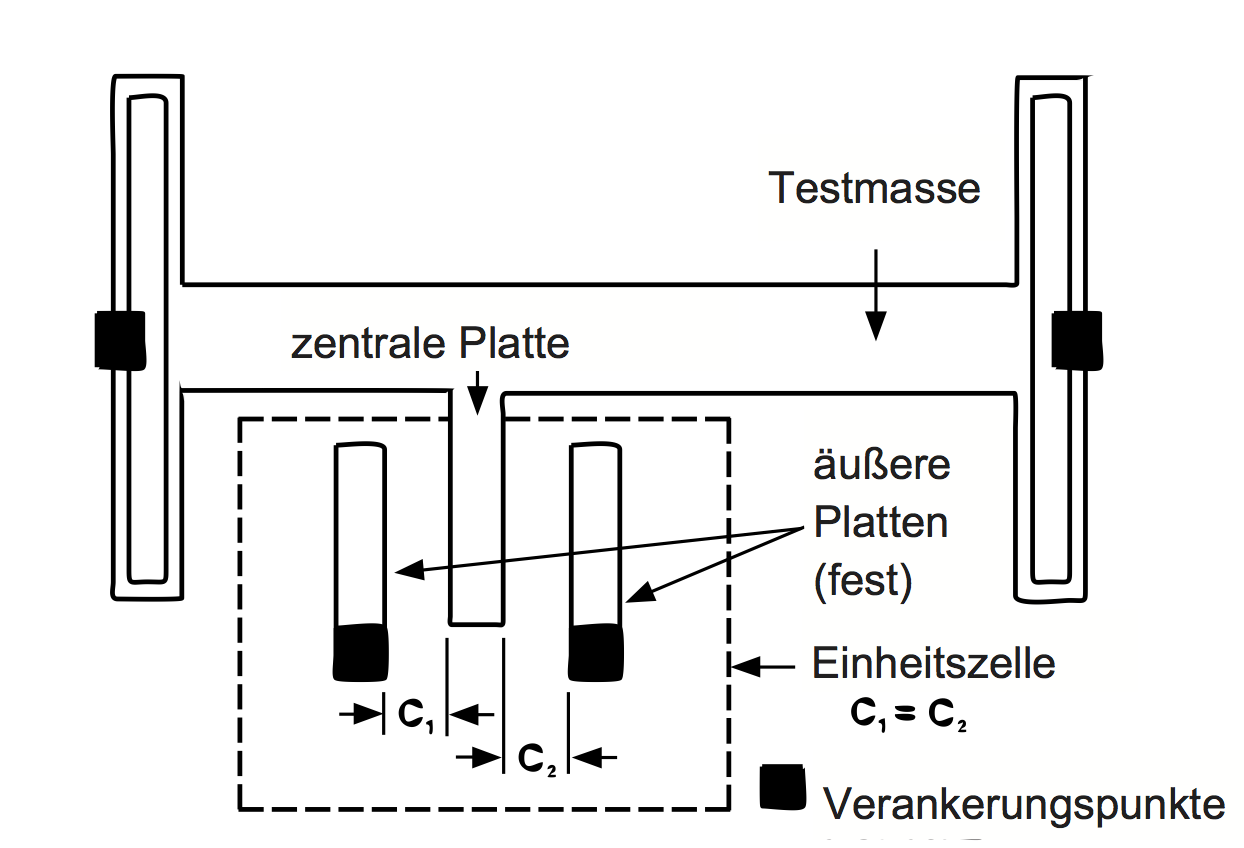
\includegraphics[width=7cm]{adxl_ruhe.png}
	}
	\subfigure[Sensor während einer externen Beschleunigung, $C_1 < C_2$] {
	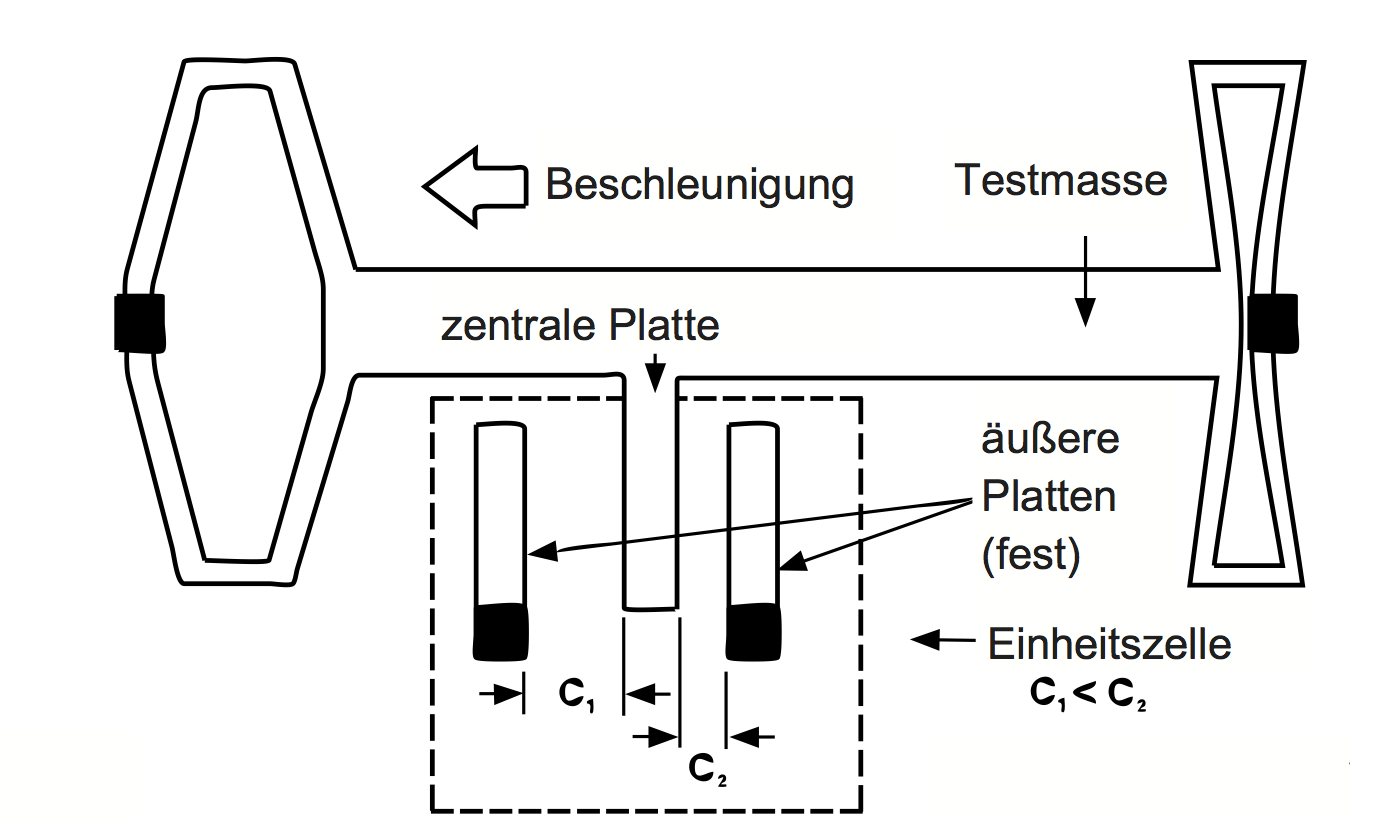
\includegraphics[width=7cm]{adxl_action.png}
 	\label{adxl_action}
	}
	\caption{Vereinfachtes Diagramm des ADXL05 \citep{Devices:1996pd}}
	\label{adxl}
\end{figure}

\begin{figure}[htb]
\centering
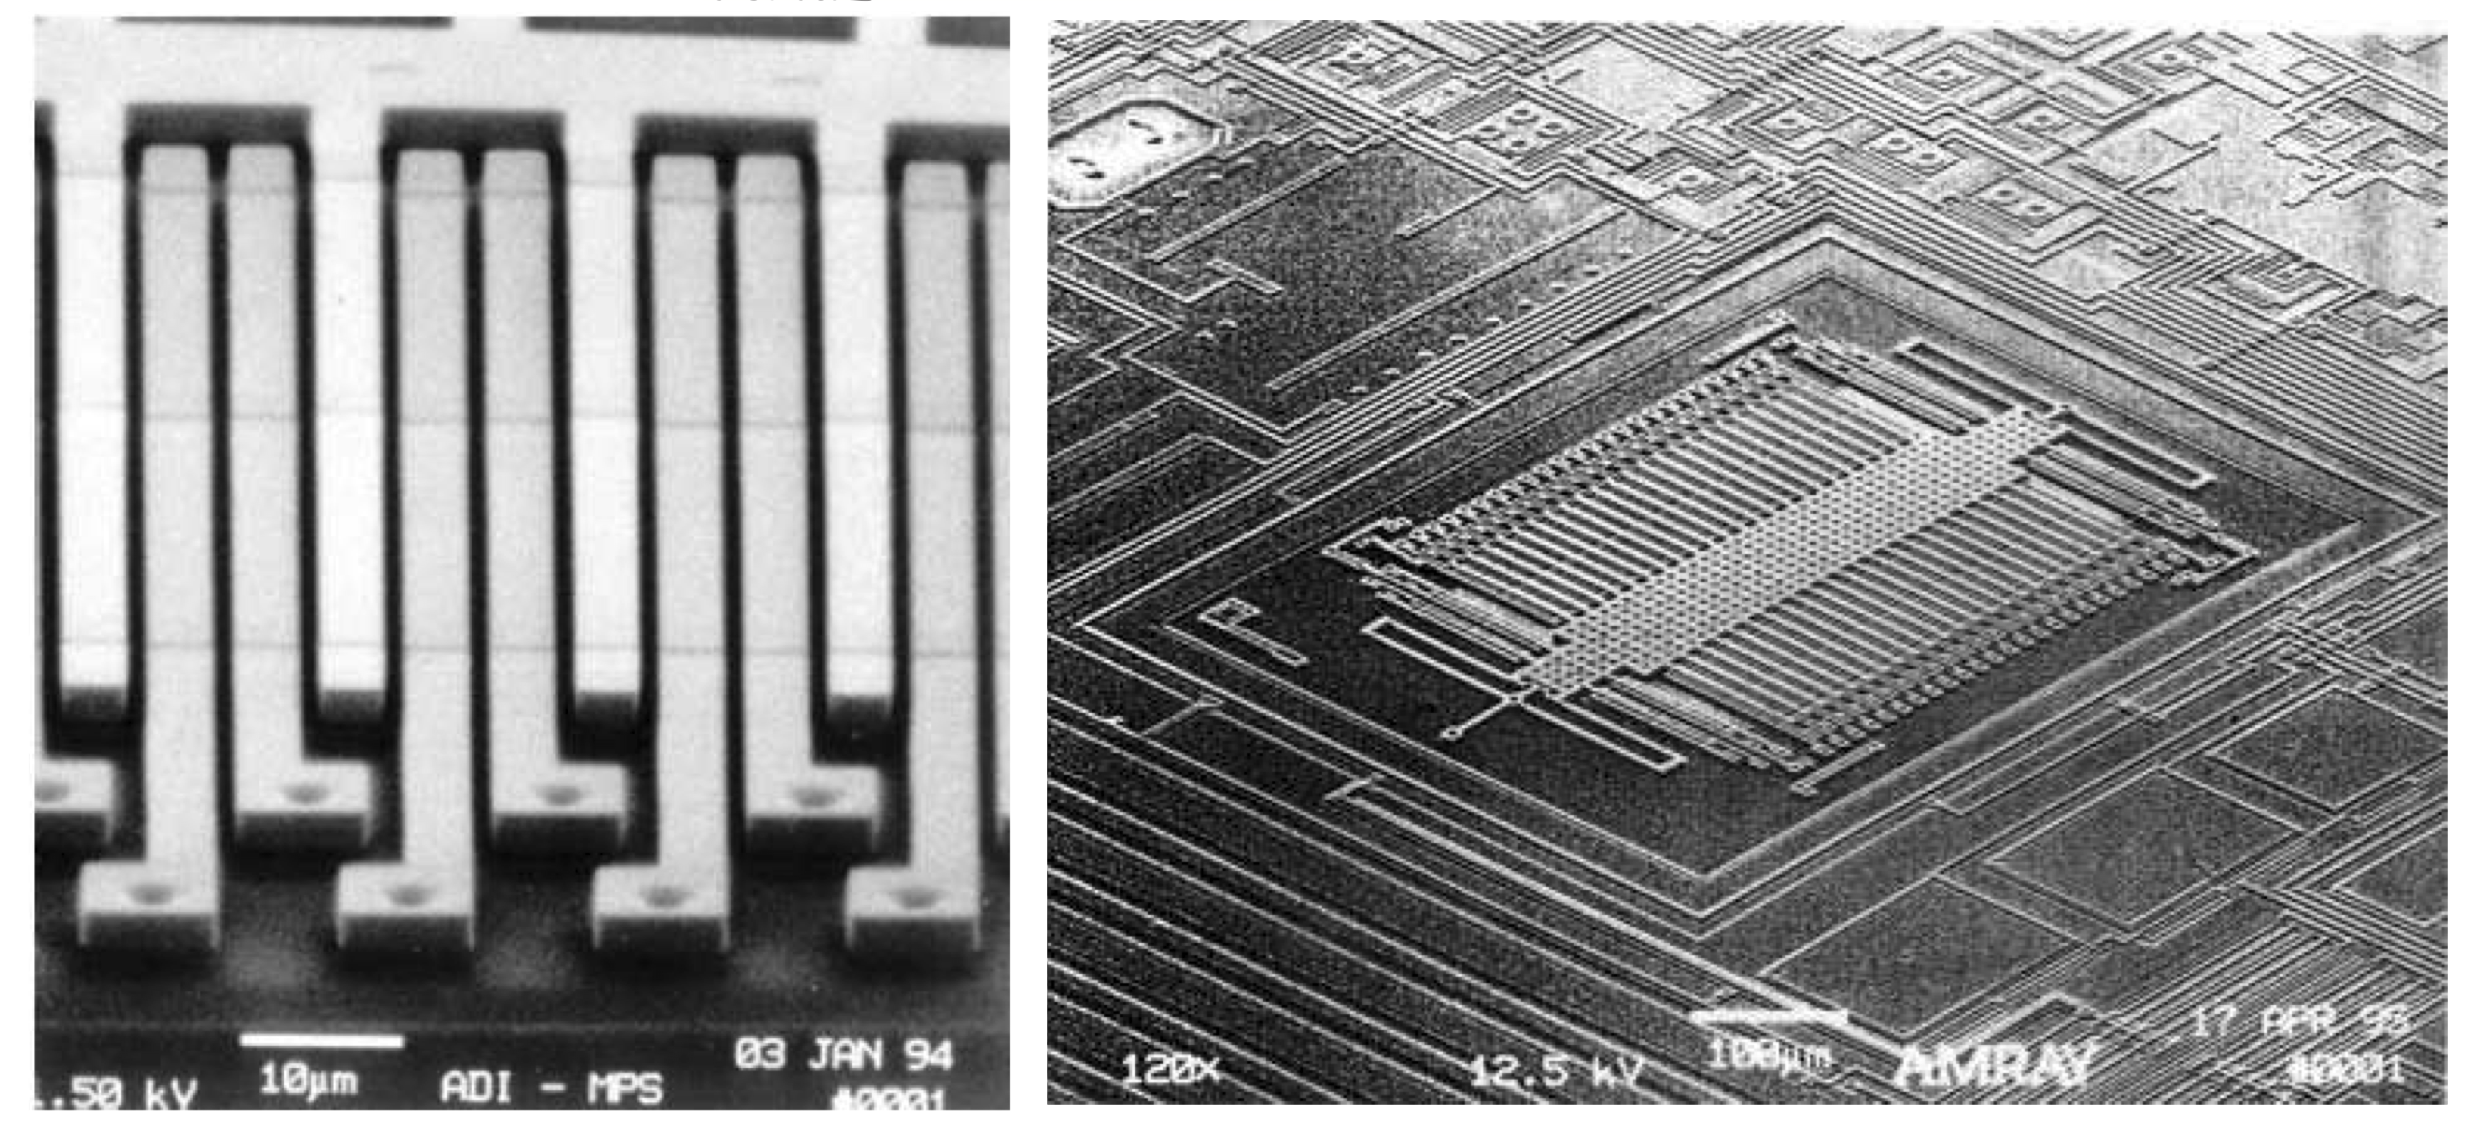
\includegraphics[scale=1]{adxl_micro.png}
\caption{ADXL05 unter dem Elektronenmikroskop, Beispiel für einen kapazitativen MEMS Beschleunigungssensor mit 46 Einzelzellen \citep{Klingbeil:2006qy}.}
\label{adxl_micro}
\end{figure}



Die Auslenkung lässt sich auch über eine Kapazitätsmessung bestimmen, wenn man je eine Elektrode an der Testmasse und am fixen Referenzpunkt anbringt \citep{S.J.-Sherman:1992ul}. Eine mögliche Realisierung ist in Abbildung \ref{adxl} a,b zu sehen: Es handelt sich um einen sogenannten Differentialkondensatorsensor \citep{:2002fk}. \\
Die seismische Masse befindet sich zwischen zwei fest verankerten Platten, die zusammen zwei Kondensatoren $C_1$ und $C_2$ bilden (Abb. \ref{adxl_ruhe}). Eine auftretende Beschleunigung führt also zu einer Auslenkung der Mittelelektrode des Kondensatorenpaares (seismische Masse) um die Länge $\pm x$ und damit zu einer symmetrischen Kapazitätsänderung um $\pm \Delta C$ (Abb. \ref{adxl_action}). Dieser Aufbau ist eine sogenannte Einzelzelle. In einem Sensor befinden sich viele Einzelzellen, um die Kapazitätsvariation und damit die Sensibilität zu erhöhen (Abb. \ref{adxl_micro}

Um diese Variation in ein elektrisches Ausgangssignal umzusetzen, wird eine sogenannte Brückenschaltung verwendet (Abb. \ref{bruecke}).

\begin{figure}[H]
\centering
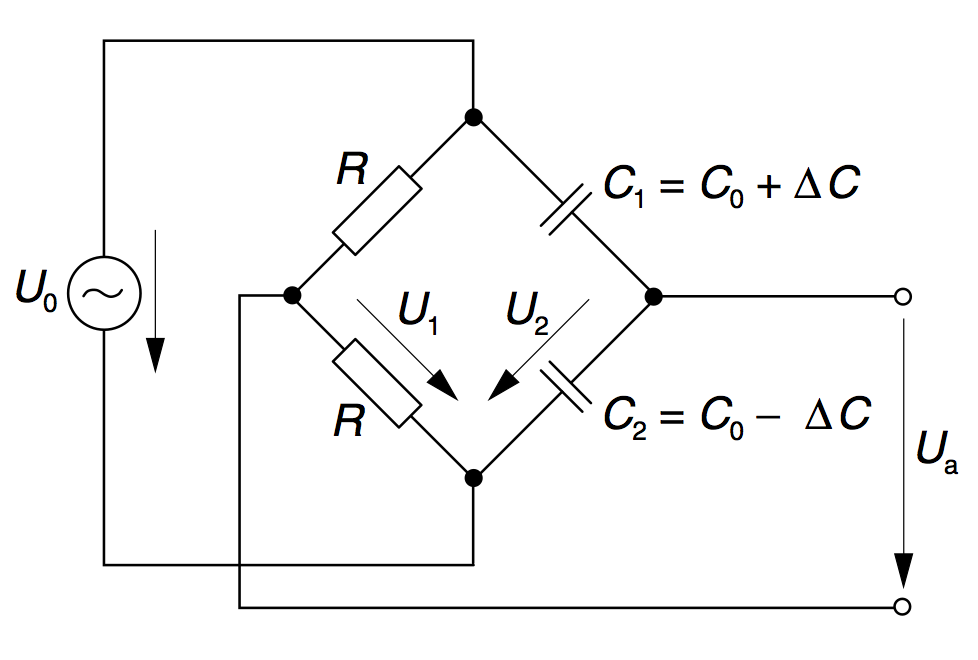
\includegraphics[scale=2]{schaltung_beschleunigungssensor.png}
\caption{Brückenschaltung mit Differentialkondensator (Die mit $U_a$ verbundenen Elektroden von $C_1$ und $C_2$ bilden eine gemeinsame Platte) \citep{:2002fk}}
\label{bruecke}
\end{figure}

Die folgende Herleitung ist aus \citep{:2002fk} entnommen:

Wird eine Wechselspannung an die Brücke angelegt, so ergibt sich nach der Spannungsteilerregel für den Ausgang $U_a$:

\begin{equation}
U_a = U_1 - U_2 = U_0 \frac{R}{2 R} - U_0 \dfrac{\dfrac{1}{j \omega C_2} } { \dfrac{1} {j \omega C_2} + \dfrac{1}{j \omega C_1} }
\end{equation}

Durch Kürzen ergibt sich:

\begin{equation}
U_a = \frac{U_0}{2} - U_0 \dfrac{\dfrac{1}{C_2}}{\dfrac{1}{C_2} + \dfrac{1}{C_1}} = U_0 \left( \frac{1}{2} - \frac{C_1}{C_2 + C_1} \right) = \frac{U_0}{2} \left( \frac{C_2 - C_1}{C_2 + C_1} \right)
\end{equation}

Mit $C_1 = C_0 + \Delta C = \varepsilon _0 \cdot \varepsilon _r \cdot A / (d_0 - x )$ und $C_2 = C_0 - \Delta C = \varepsilon _0 \cdot \varepsilon _r \cdot A / (d_0 + x )$ erhält man eine lineare Abhängigkeit der Ausgangsspannung $U_a$ von der Auslenkung  $x$:

\begin{equation}
U_a = - U_0 \frac{x}{2 d_0}
\end{equation}\\


Diese Spannung lässt sich nun digitalisieren und auslesen. In vielen MEMS Bausteinen ist bereits ein integrierter Analog Digital Wandler eingebaut, sodass die Messwerte direkt digital abrufbar sind. 

\newpage

\section{Entwicklung des Schwingungsmesssystems: Prototyp (BMA180)}

Um abschätzen zu können wie groß die auftretenden Beschleunigungen an der Radarantenne sind, habe ich damit begonnen einen günstigen und einfach zu verwendenden Prototypen zu entwickeln. Letzteres ist vor Allem wichtig, um entscheiden zu können, für welchen Messbereich und welche Frequenzen der eigentliche Sensor ausgelegt sein muss. \\

\subsection{Bosch BMA180}
\begin{figure}[ht]
\centering
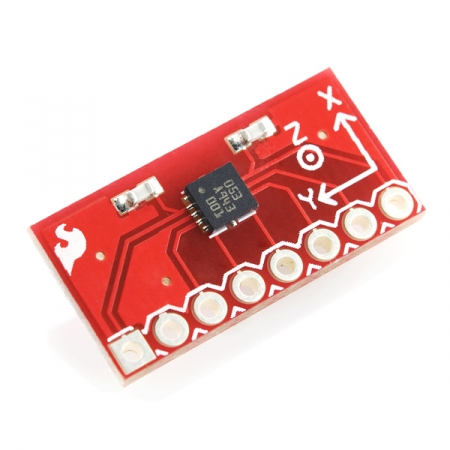
\includegraphics[scale=.4]{hardwareimages/bma180_breakout.jpg}
\caption{BMA180 Breakoutboard von Sparkfun}
\label{bma180_breakout}
\end{figure}

Die Wahl fiel auf einen digitalen, dreiachsigen MEMS Beschleunigungssensor \textit{Bosch BMA180}. Er verfügt über einen eingebauten 14-bit Analog-Digital Wandler und sieben per Software verstellbaren Messbereiche von $\pm1$ bis $\pm16$g.
Die Kommunikation kann über SPI (Serial Peripheral Interface)  oder I$^2$C (Inter-Integrated Circuit) erfolgen.

Ich nutze ein Breakoutboard von Sparkfun (Abb. \ref{bma180_breakout}), welches die IC Pins (SMD Technik) mit praktische Lötösen verbindet. Außerdem sind bereits zwei spannungsstabilisierende Kondensatoren mit auf der Platine verbaut.

\subsection{Arduino}

\begin{figure}[ht]
\centering
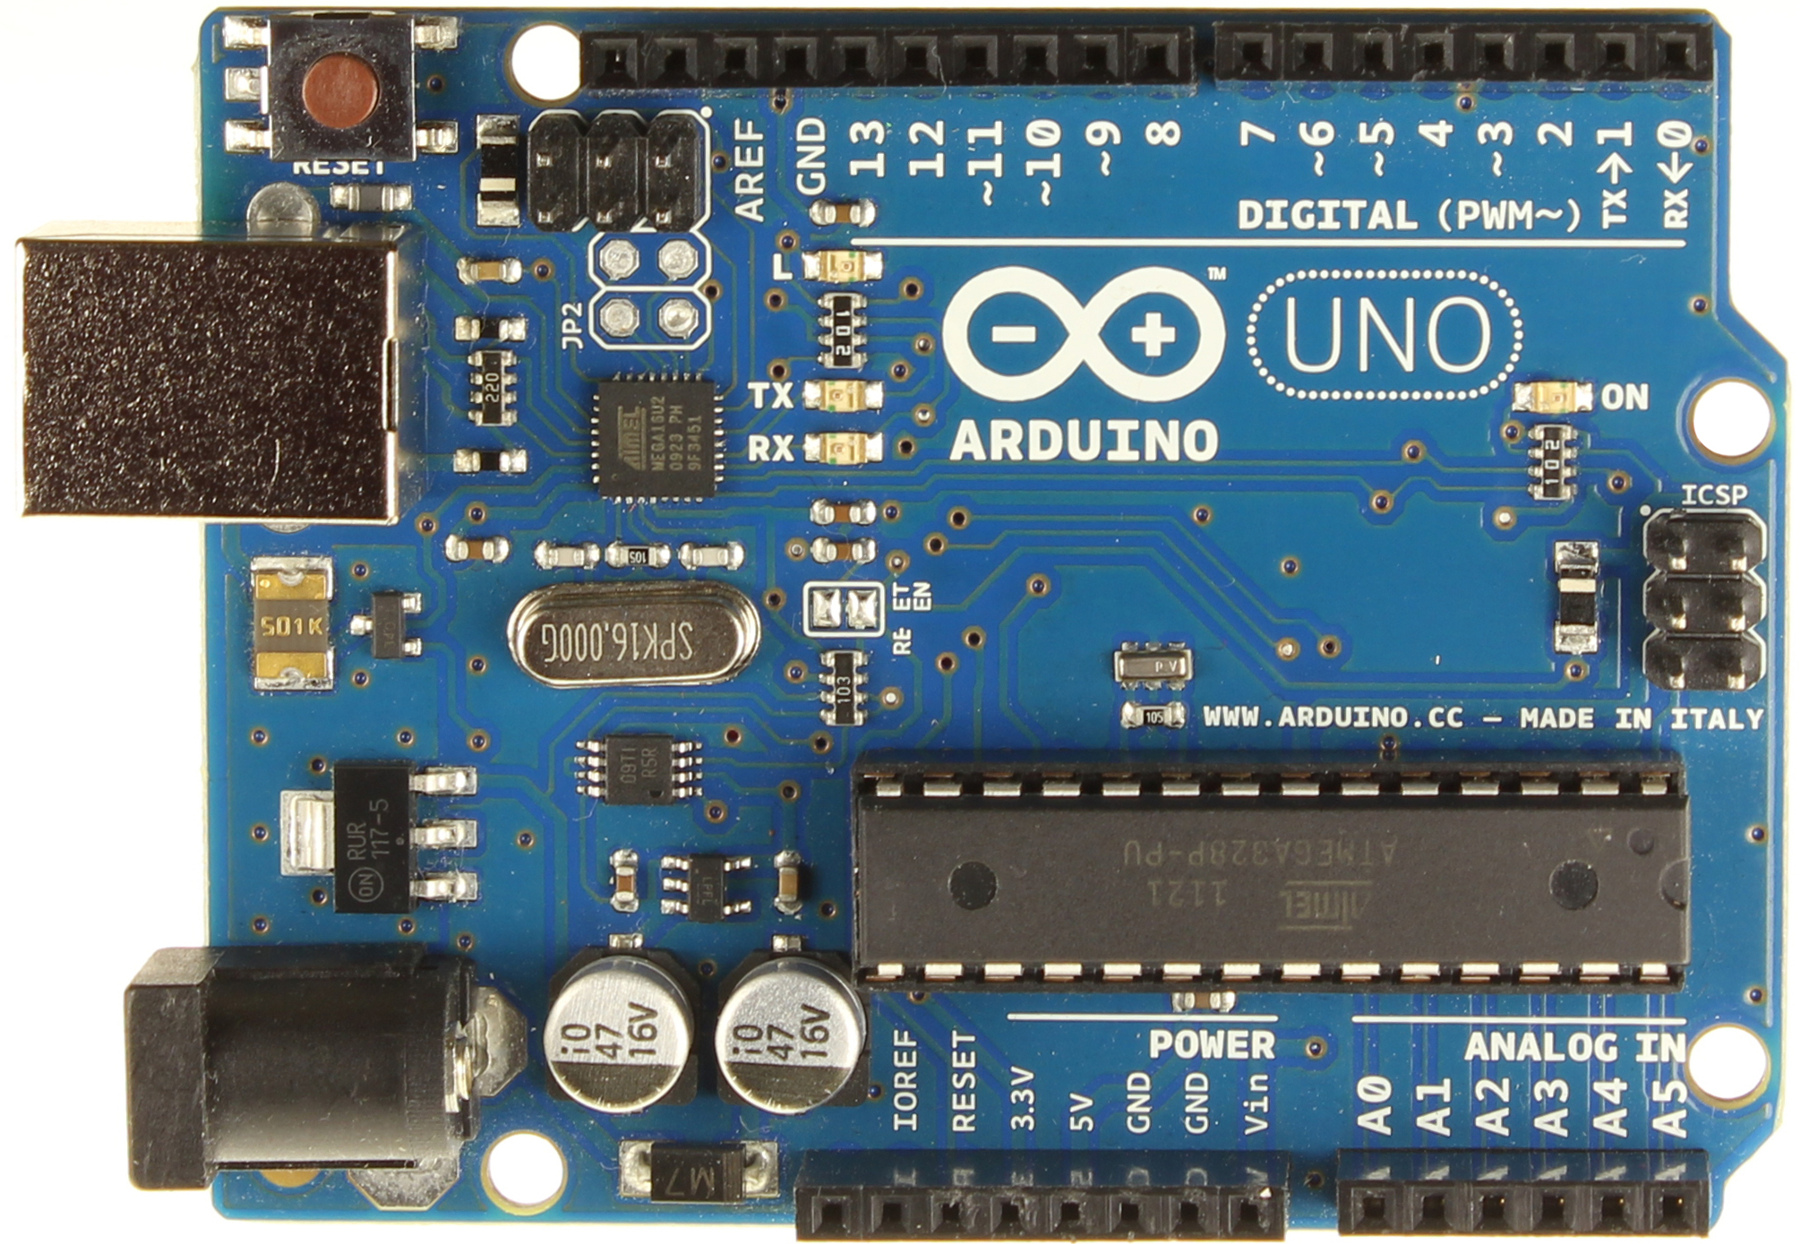
\includegraphics[scale=.2]{hardwareimages/ArduinoUno_R3_Front.jpg}
\caption{Arduino UNO}
\label{Arduino}
\end{figure}


Arduino ist eine auf ATmega Mikroprozessoren basierende Open-Source Entwicklungsplattform zur Verarbeitung von analogen und digitalen Signalen. Die Programmierung kann über eine eigene Entwicklungsumgebung in einer an \textit{Processing\footnote{processing.org}} angelehnten Sprache erfolgen, die im Prinzip ein vereinfachtes C/C++ darstellt.\\
Die Plattform ist auf Prototyping und Experimente ausgelegt. Es ist bereits ein Bootloader vorinstalliert, so kann die Programmierung direkt über die serielle Schnittstelle erfolgen. Die Boards machen die meisten Pins des ATmegas für eigene Schaltungen verfügbar, in den gängigen Boards sind das 14 Pins, die frei als Ein- oder Ausgänge genutzt werden können.
Die Stromversorgung kann über USB oder eine externe 5V Quelle erfolgen. Als Kommunikationsinterfaces werden SPI, ICSP (In-Circuit Serial Programming) und I$^2$C angeboten.\\
Der ATmega arbeitet mit 16 MHz und hat einen geringen Energieverbrauch.


\subsection{Schnittstellen}

\subsubsection{I$^2$C}
Zur Kommunikation zwischen Beschleunigungssensor und Arduino habe ich den  I$^2$C Bus \citep{:2012fj} gewählt.
Dabei handelt es sich um einen von Phillips entwickelten seriellen Datenbus, der ursprünglich entwickelt wurde, um Chips in Fernsehgeräten steuern zu können. Inzwischen ist das Patent ausgelaufen und er wird in vielen Hardwareprojekten verwendet, da er sehr einfach zu verstehen und zu verwenden ist. 

Ich benutze die Arduino Wire Library \citep{:2012vn}, welche die gesamte Kommunikation über I$^2$C steuert und einfache Funktionsaufrufe, wie zum Beispiel Senden und Empfangen, zur Verfügung stellt.

\subsubsection{Serieller Port}
Zum einfachen Anschluss des Arduinos an einen PC oder Datenlogger wird eine serielle Schnittstelle nach RS232 verwendet. Auf dem Arduino befindet sich ein ATmega16U2, welcher die seriellen Signale in USB umwandelt und dafür sorgt, dass der Arduino am PC als virtueller COM-Port erscheint.

\newpage
\subsection{Aufbau und Schaltung}

\subsubsection{Testaufbau}

Um die korrekte Verschaltung zu überprüfen und die Software für das Auslesen der Daten zu zu entwickeln, habe ich zunächst auf dem Breadboard gearbeitet. Der dazu verwendete Schaltplan ist in Abbildung \ref{schematics} zu sehen.

Da der Sensor sowohl im I$^2$C- sowie im SPI-Modus betrieben werden kann, ist es notwendig, den Modus bereits bei der Verschaltung einzustellen. Über den CS Pin (Pin 4) ist dies möglich. Schaltet man ihn auf High (3.3V), so benutzt der Chip I$^2$C, verbindet man ihn mit GND, so wird ISP verwendet. Je nach Modus haben die Pins unterschiedliche Funktionen. In Tabelle \ref{i2cmode} sind die verschiedenen Konfigurationen aufgeführt.

Pin 6 legt im von mir benutzten I$^2$C Modus die Adresse des Chips fest. Ist dieser auf Low (GND), so ist die Adresse 0x40.



\begin{figure}[htb]
	\centering
	\subfigure[Testaufbau auf dem Breadboard] {
		\label{breadboard}
		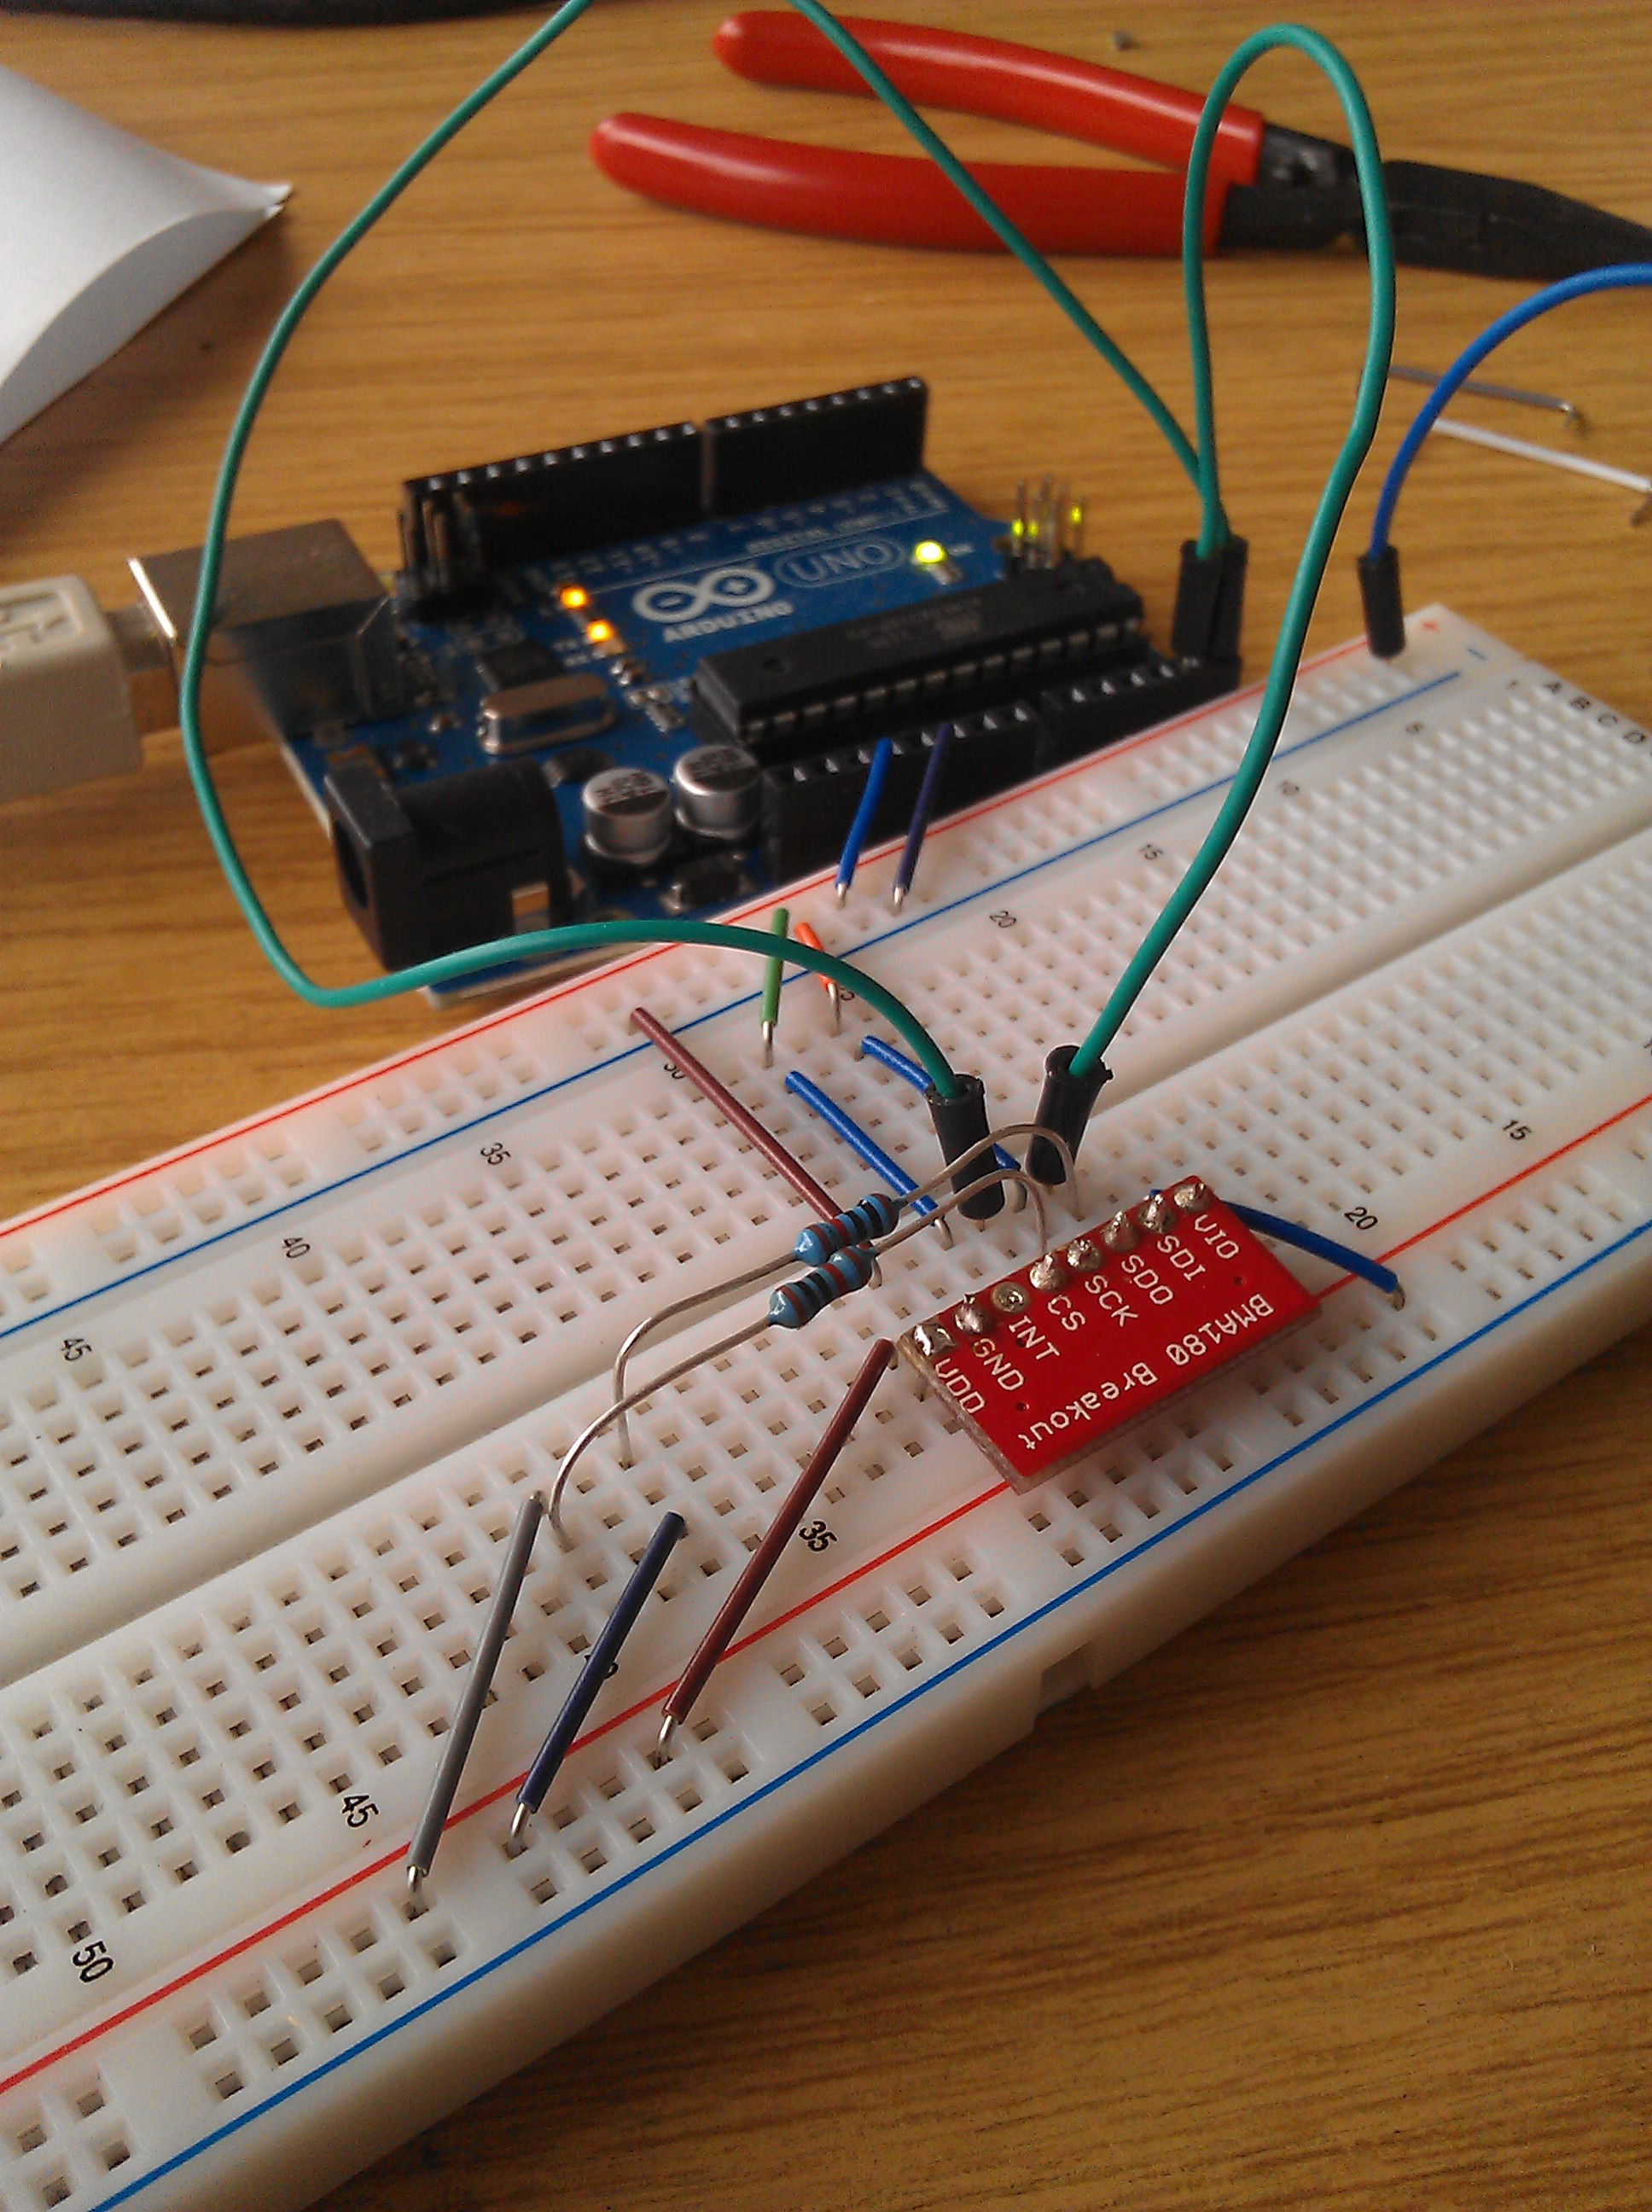
\includegraphics[width=7cm]{hardwareimages/breadboard.jpg}
	}
	\subfigure[Testplatine am Radar] {
	\includegraphics[width=7cm]{hardwareimages/testaufbau.png}
 	\label{testaufbau}
	}
	\caption{Testaufbau des Sensors}
	\label{testaufbaufigure}
\end{figure}


\begin{table}[htb]
\begin{tabular}{@{}lll@{}}      
    	\cmidrule(r){1-2}\morecmidrules\cmidrule(r){1-2}
       	Pin & SPI mode & I2C mode\\
      	\midrule
 	7 & SDI input & SDA birectional (!) \\ 
 	6 & SDO output & ADDR adress bit, input \\
 	5 & SCLK input & SCL input \\
 	4 & CSB chip select, input & I2C mode select, input \\
 	 \addlinespace
 	 \bottomrule
 \end{tabular}
\caption{BMA180 Pinbelegung für SPI und I$^2$C Modes \citep{Sensortec:2009rt}}
\label{i2cmode}
\end{table}


\begin{figure}[ht]
\centering
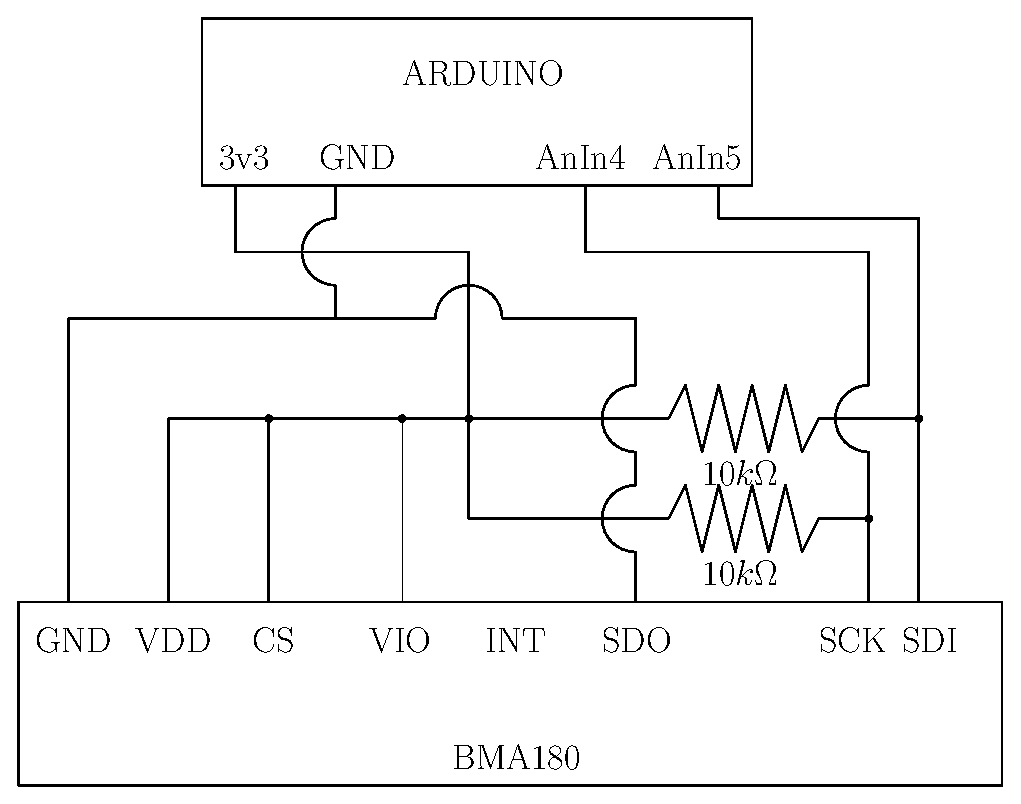
\includegraphics[scale=.6]{schematics.eps}
\caption{Schaltplan Testaufbau. Der Interrupt ist nicht verbunden, VDD und CS sind auf 3.3V geschaltet, GND und SDO auf die Masse des Arduinos gezogen, die I$^2$C Datenleitungen SCK und SDI sind mit den Arduinopins A4 und A5 verbunden, wobei zusätzlich 10k$\Omega$ Pull-Up-Widerstände eingebaut sind.}
\label{schematics}
\end{figure}


\newpage
\subsubsection{Fester Aufbau}

Um das System praktisch nutzen zu können muss es natürlich fest aufgebaut werden und mit einem Gehäuse versehen werden, das es erlaubt, ihn fest an einem Testobjekt anzubringen und ihn gleichzeitig vor Schäden durch mechanische oder witterungsbedingte Einflüsse schützt.

Um die eigentliche Sensoreinheit möglichst kompakt zu halten, habe ich mich entschieden, den Beschleunigungssensor vom Arduino zu trennen und auf eine kleine Lochrasterplatine zu löten. Diese wird in einen festen Block aus Polyurethanharz\footnote{OPTICALLY CLEAR POLYURETHANE, RS COMPONENTS, RS 195-984A} eingegossen, womit sie gleichzeitig gut geschützt und leicht anzubringen ist (Abb. \ref{harz}). \\

\begin{figure}[H]
\centering
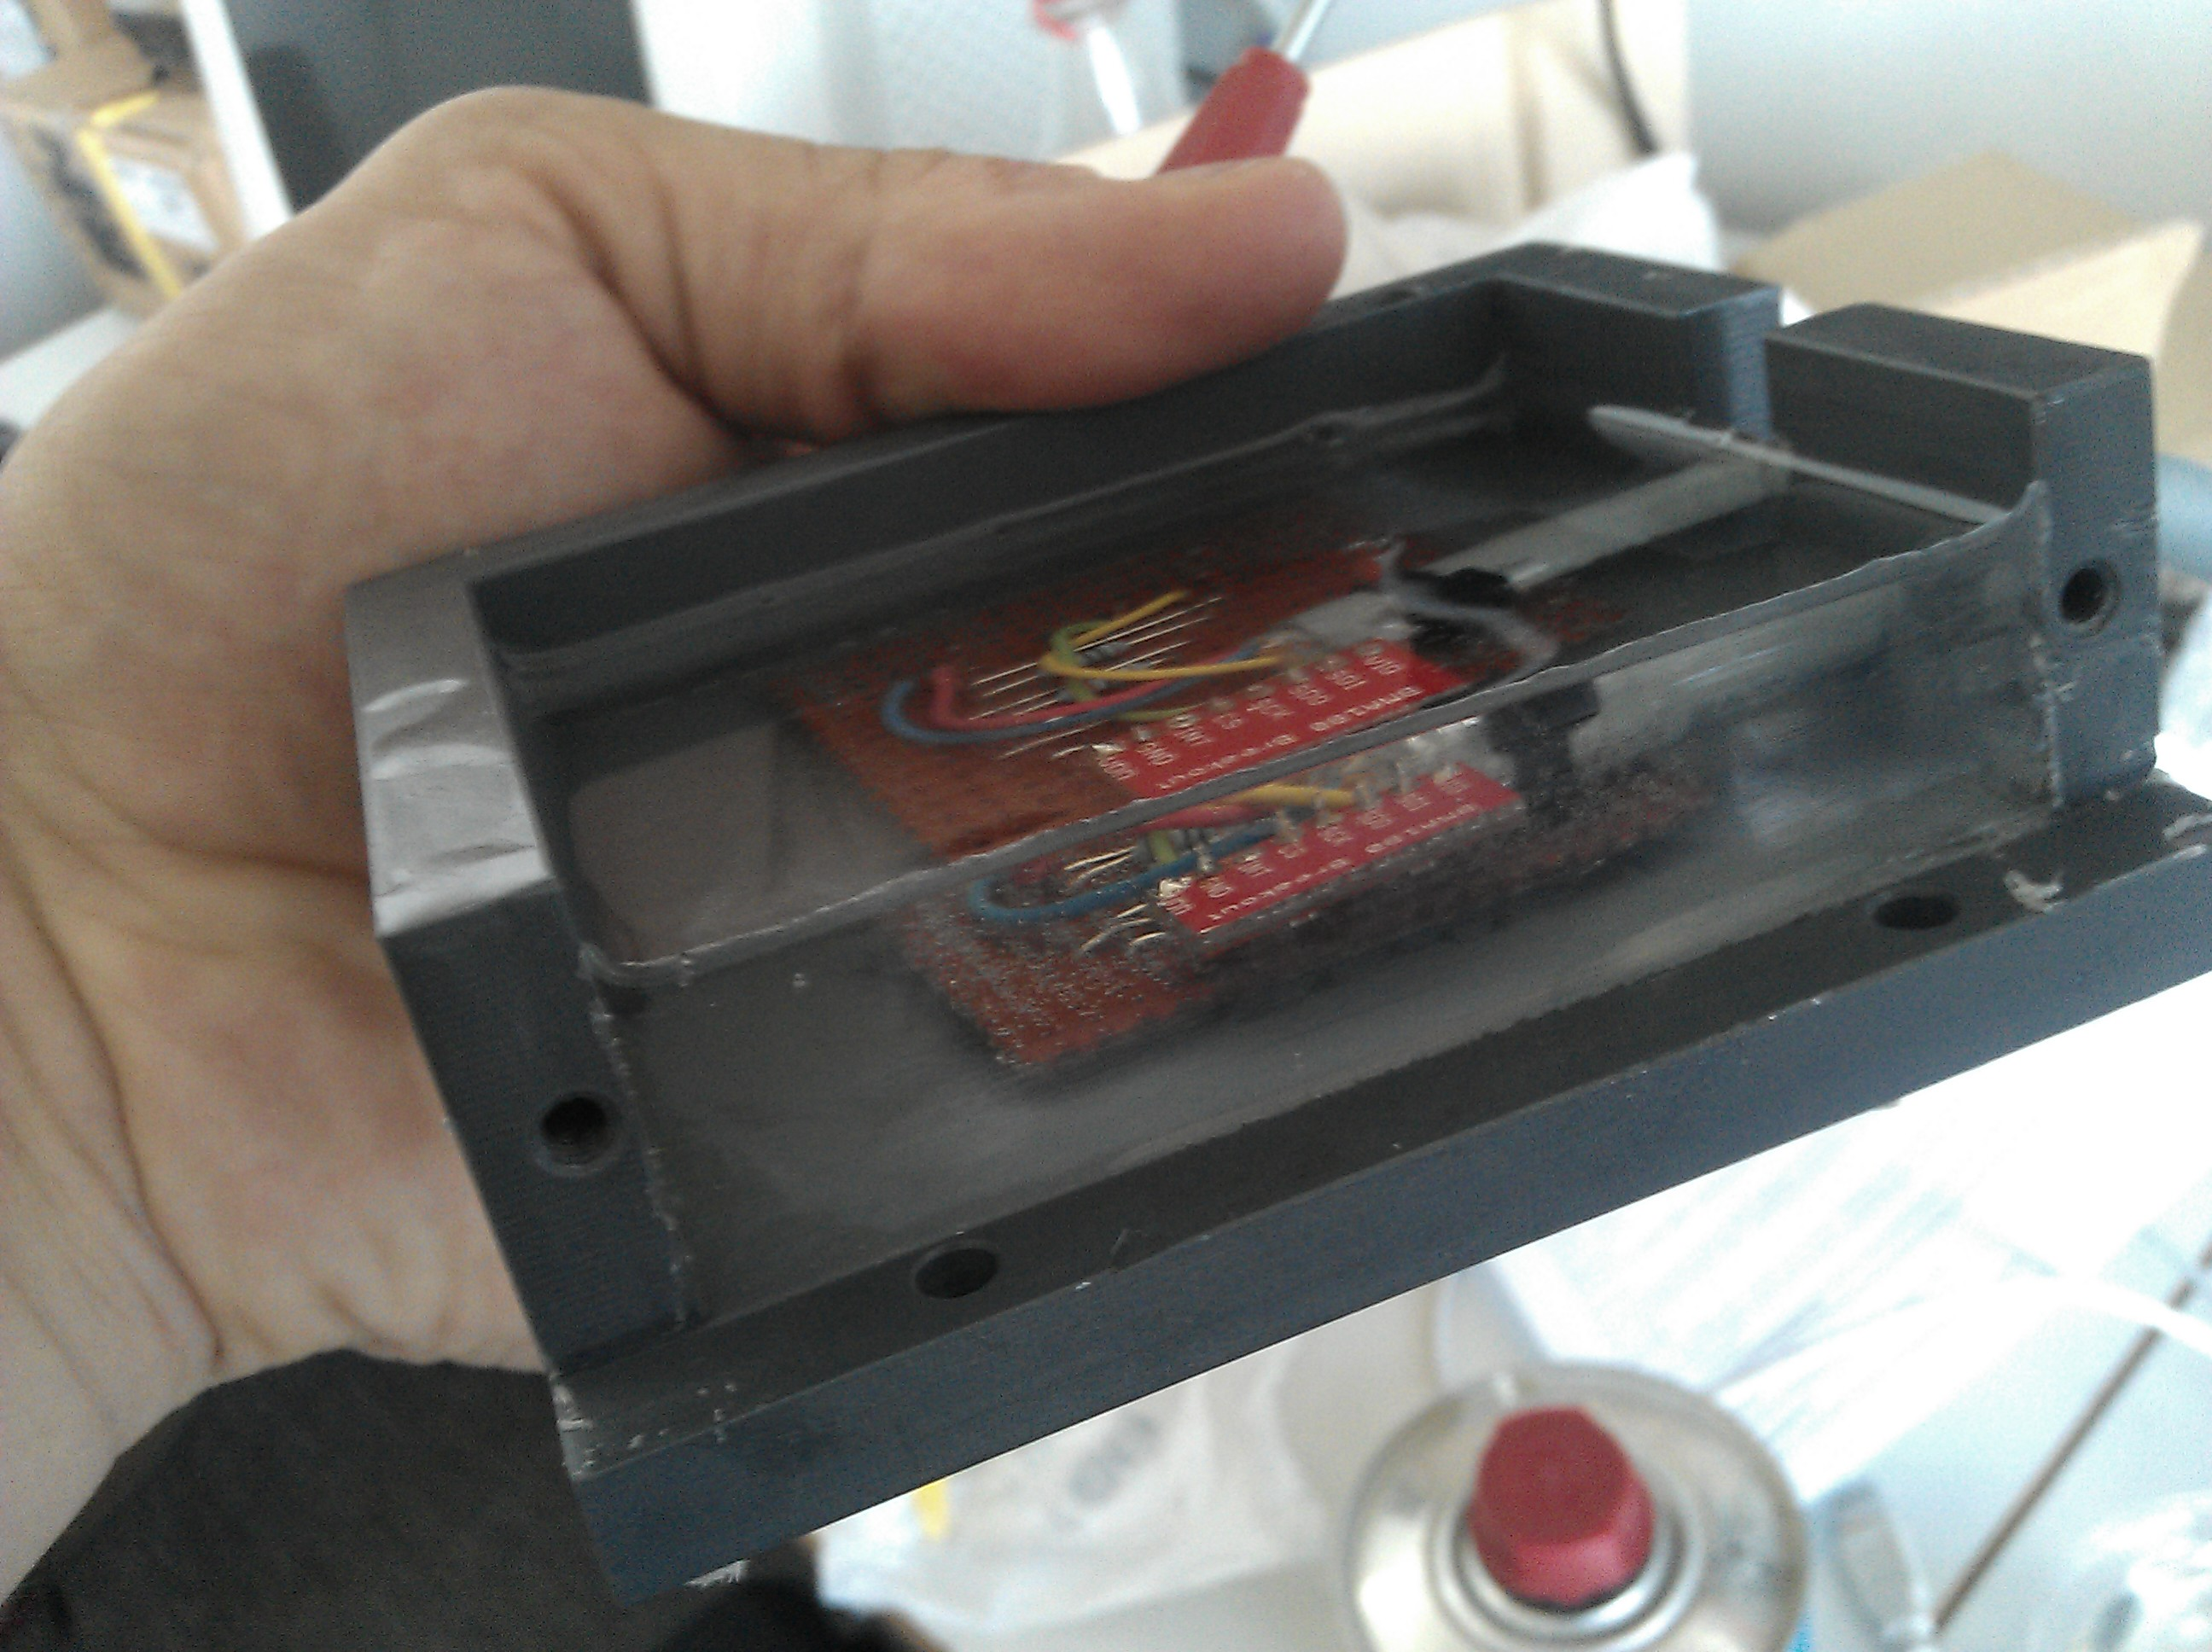
\includegraphics[scale=.14]{hardwareimages/harz.jpg}
\caption{BMA180 in Polyurethanharz eingegossen, die Kunststoffform wurde von den feinmechanischen Werkstätten des Fachbereichs Geowissenschaften gefertigt.}
\label{harz}
\end{figure}

Der Arduino ist in ein ABS Gehäuse (zum Beispiel von BOSS Endloseres) eingebaut (Abb. \ref{arduinobox} und \ref{arduinoboxregen}
Die I$^2$C Verbindung mit dem Sensor erfolgt über einen Hirschmannstecker™ mit 7 Polen, von denen 4 beschaltet sind, wie in Abbildung \ref{hirschmann_i2c} zu sehen ist.
Mit dem Logger ist der Arduino über ein USB-Kabel verbunden, über das die Kommunikation per RS232 geführt wird.

\begin{figure}[ht]
\centering
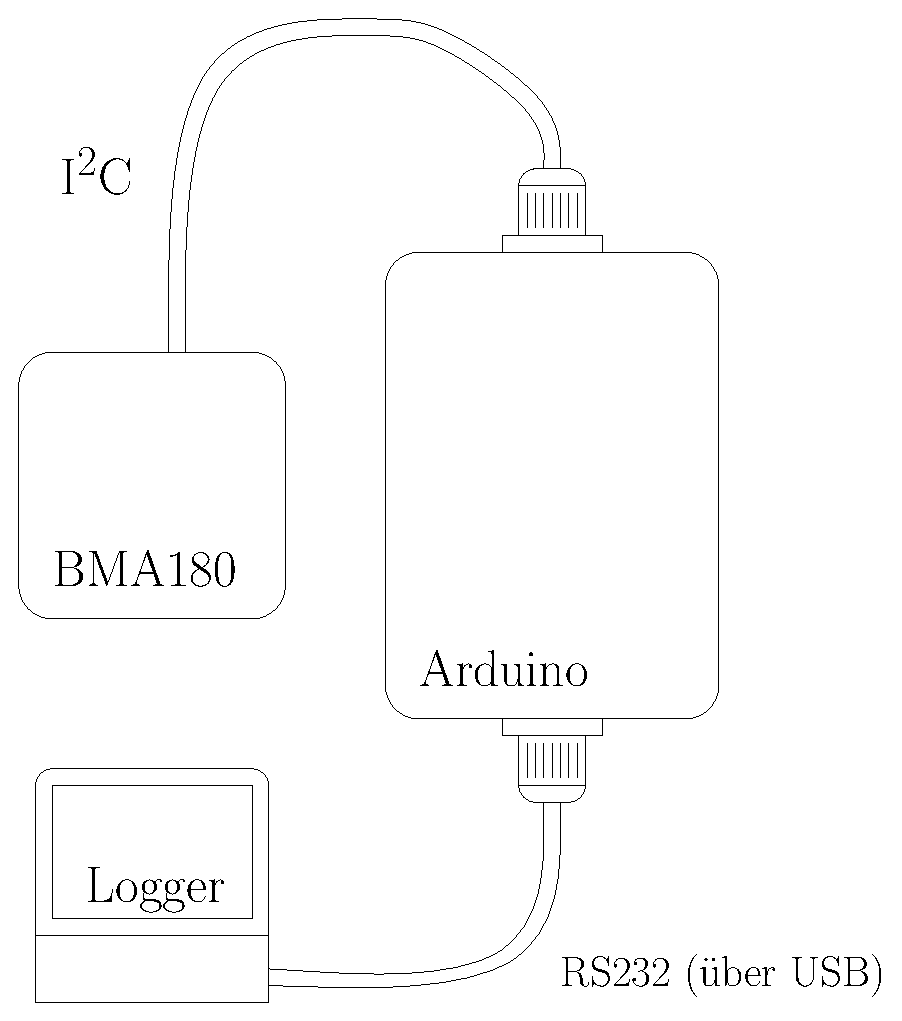
\includegraphics[scale=.8]{hardwareimages/kabel.eps}
\caption{Verbindungen zwischen BMA180, Arduino und Logger per I$^2$C bzw. RS232}
\label{kabel}
\end{figure}

\begin{figure}[H]
	\begin{minipage}[H]{8cm}
		\centering
		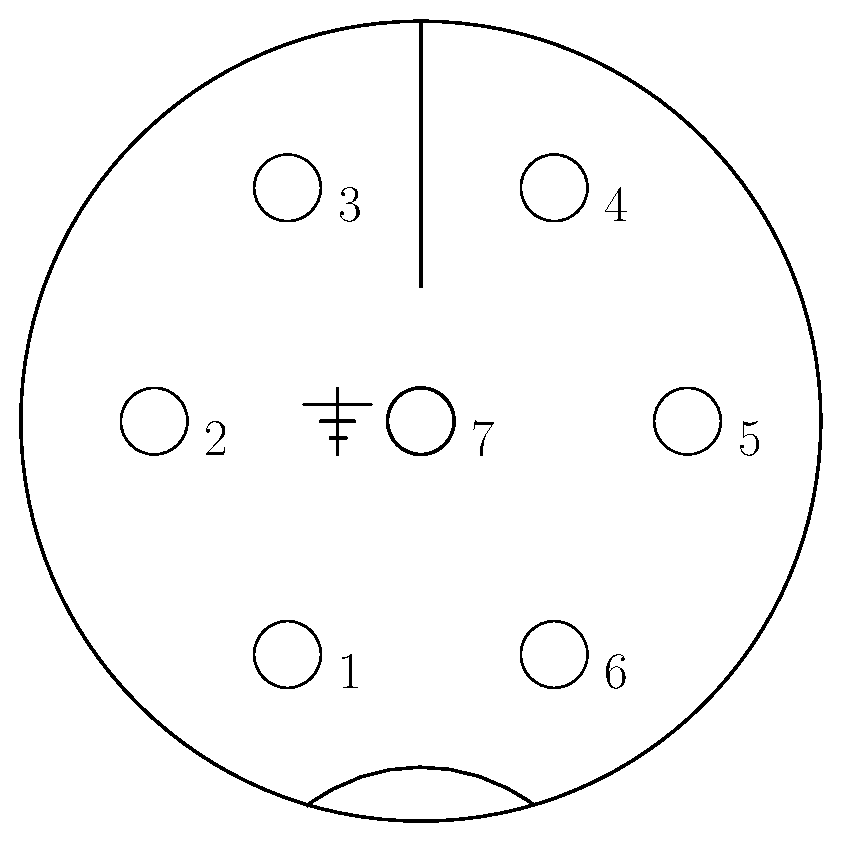
\includegraphics[scale=.5]{hardwareimages/hirschmann_i2c.eps}
	\end{minipage}
	\hfill
	\begin{minipage}[H]{8cm}
		\centering
		\begin{tabular}{@{}lllll@{}}    
      			\cmidrule(r){1-5}\morecmidrules\cmidrule(r){1-5}
       			Pin & I2C & Arduino & BMA180 & Farbe\\
      			\midrule
 			1 & 3.3V & 3.3V & VDD & Rot \\ 
 			2 & & & &\\
 			3 & SDA & A4 & SDI & Gelb\\
 			4 & SCL & A5 & SCK & Grün\\
 			5 & & & &\\
 			6 & & & &\\
 			7 & GND & GND & GND & Schwarz\\
   			\addlinespace
   			\bottomrule
 		\end{tabular}
	\end{minipage}
	\caption{I$^2$C Beschaltung des Hirschmannsteckers™}
	\label{hirschmann_i2c}
\end{figure}


\begin{figure}[htb]
	\centering
	\subfigure[ABS Box, welche den Arduino enthält] {
		\label{arduinobox}
		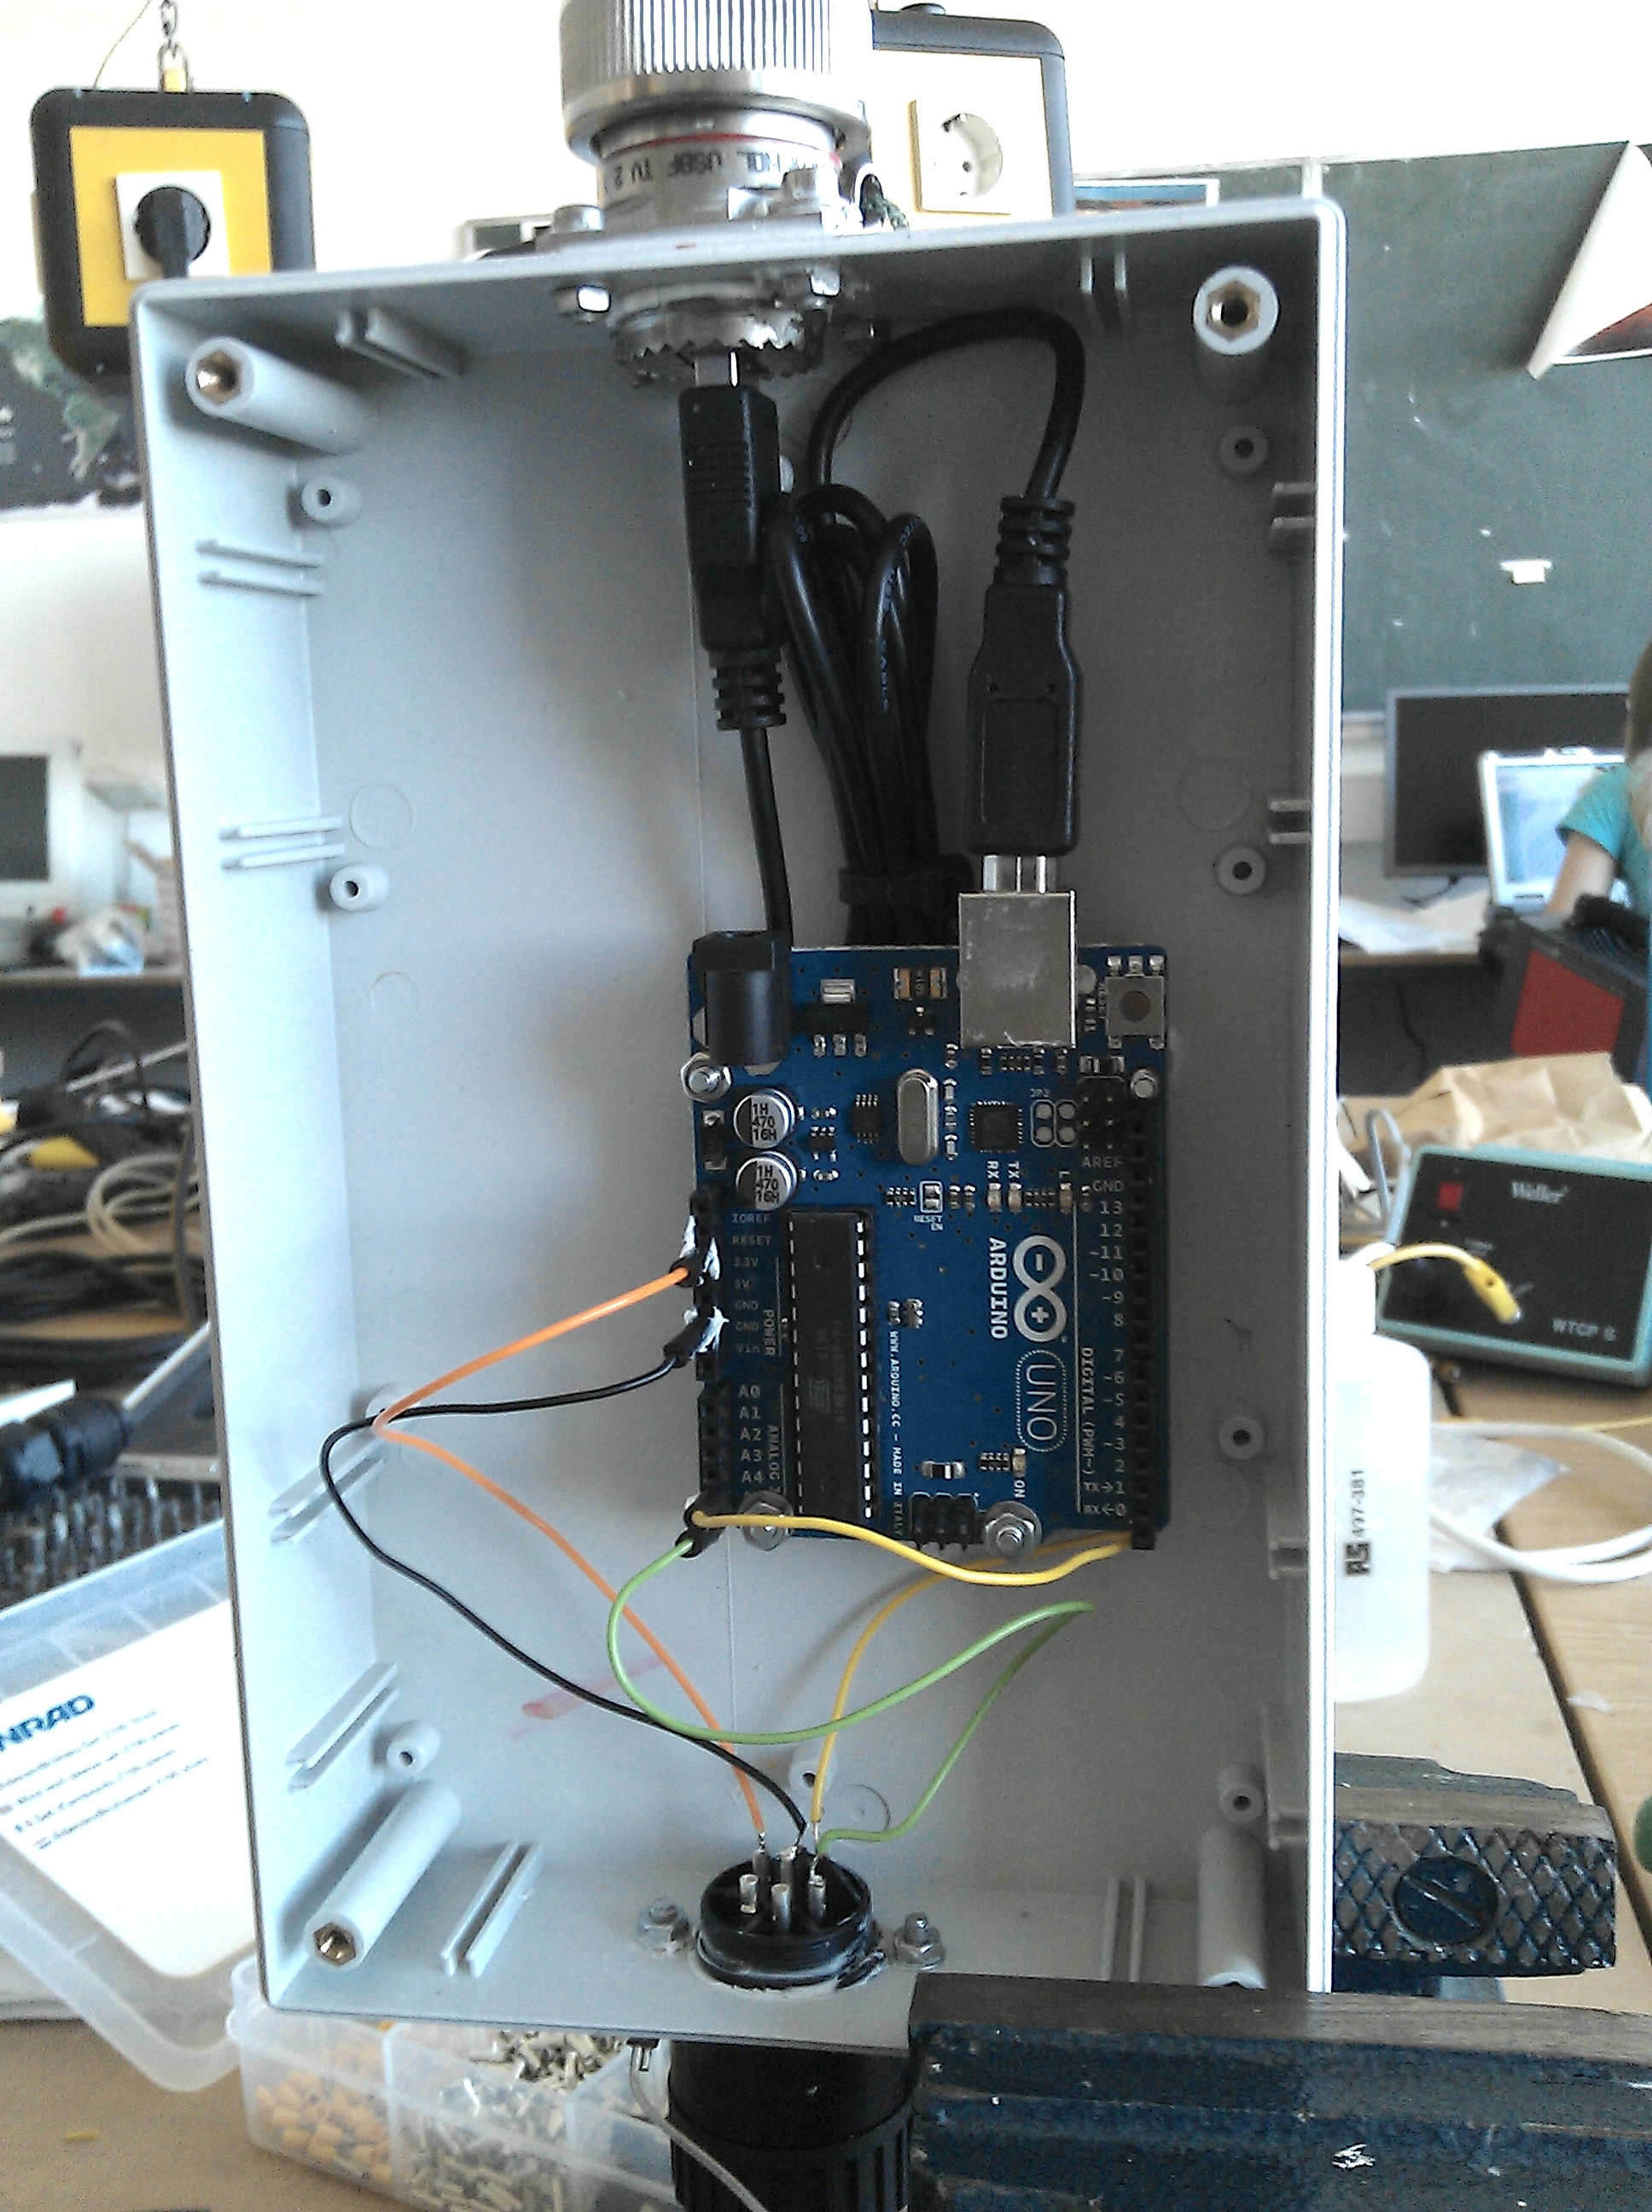
\includegraphics[width=7cm]{hardwareimages/arduinobox.jpg}
	}
	\subfigure[ABS Box, geschlossen im Witterungstest] {
	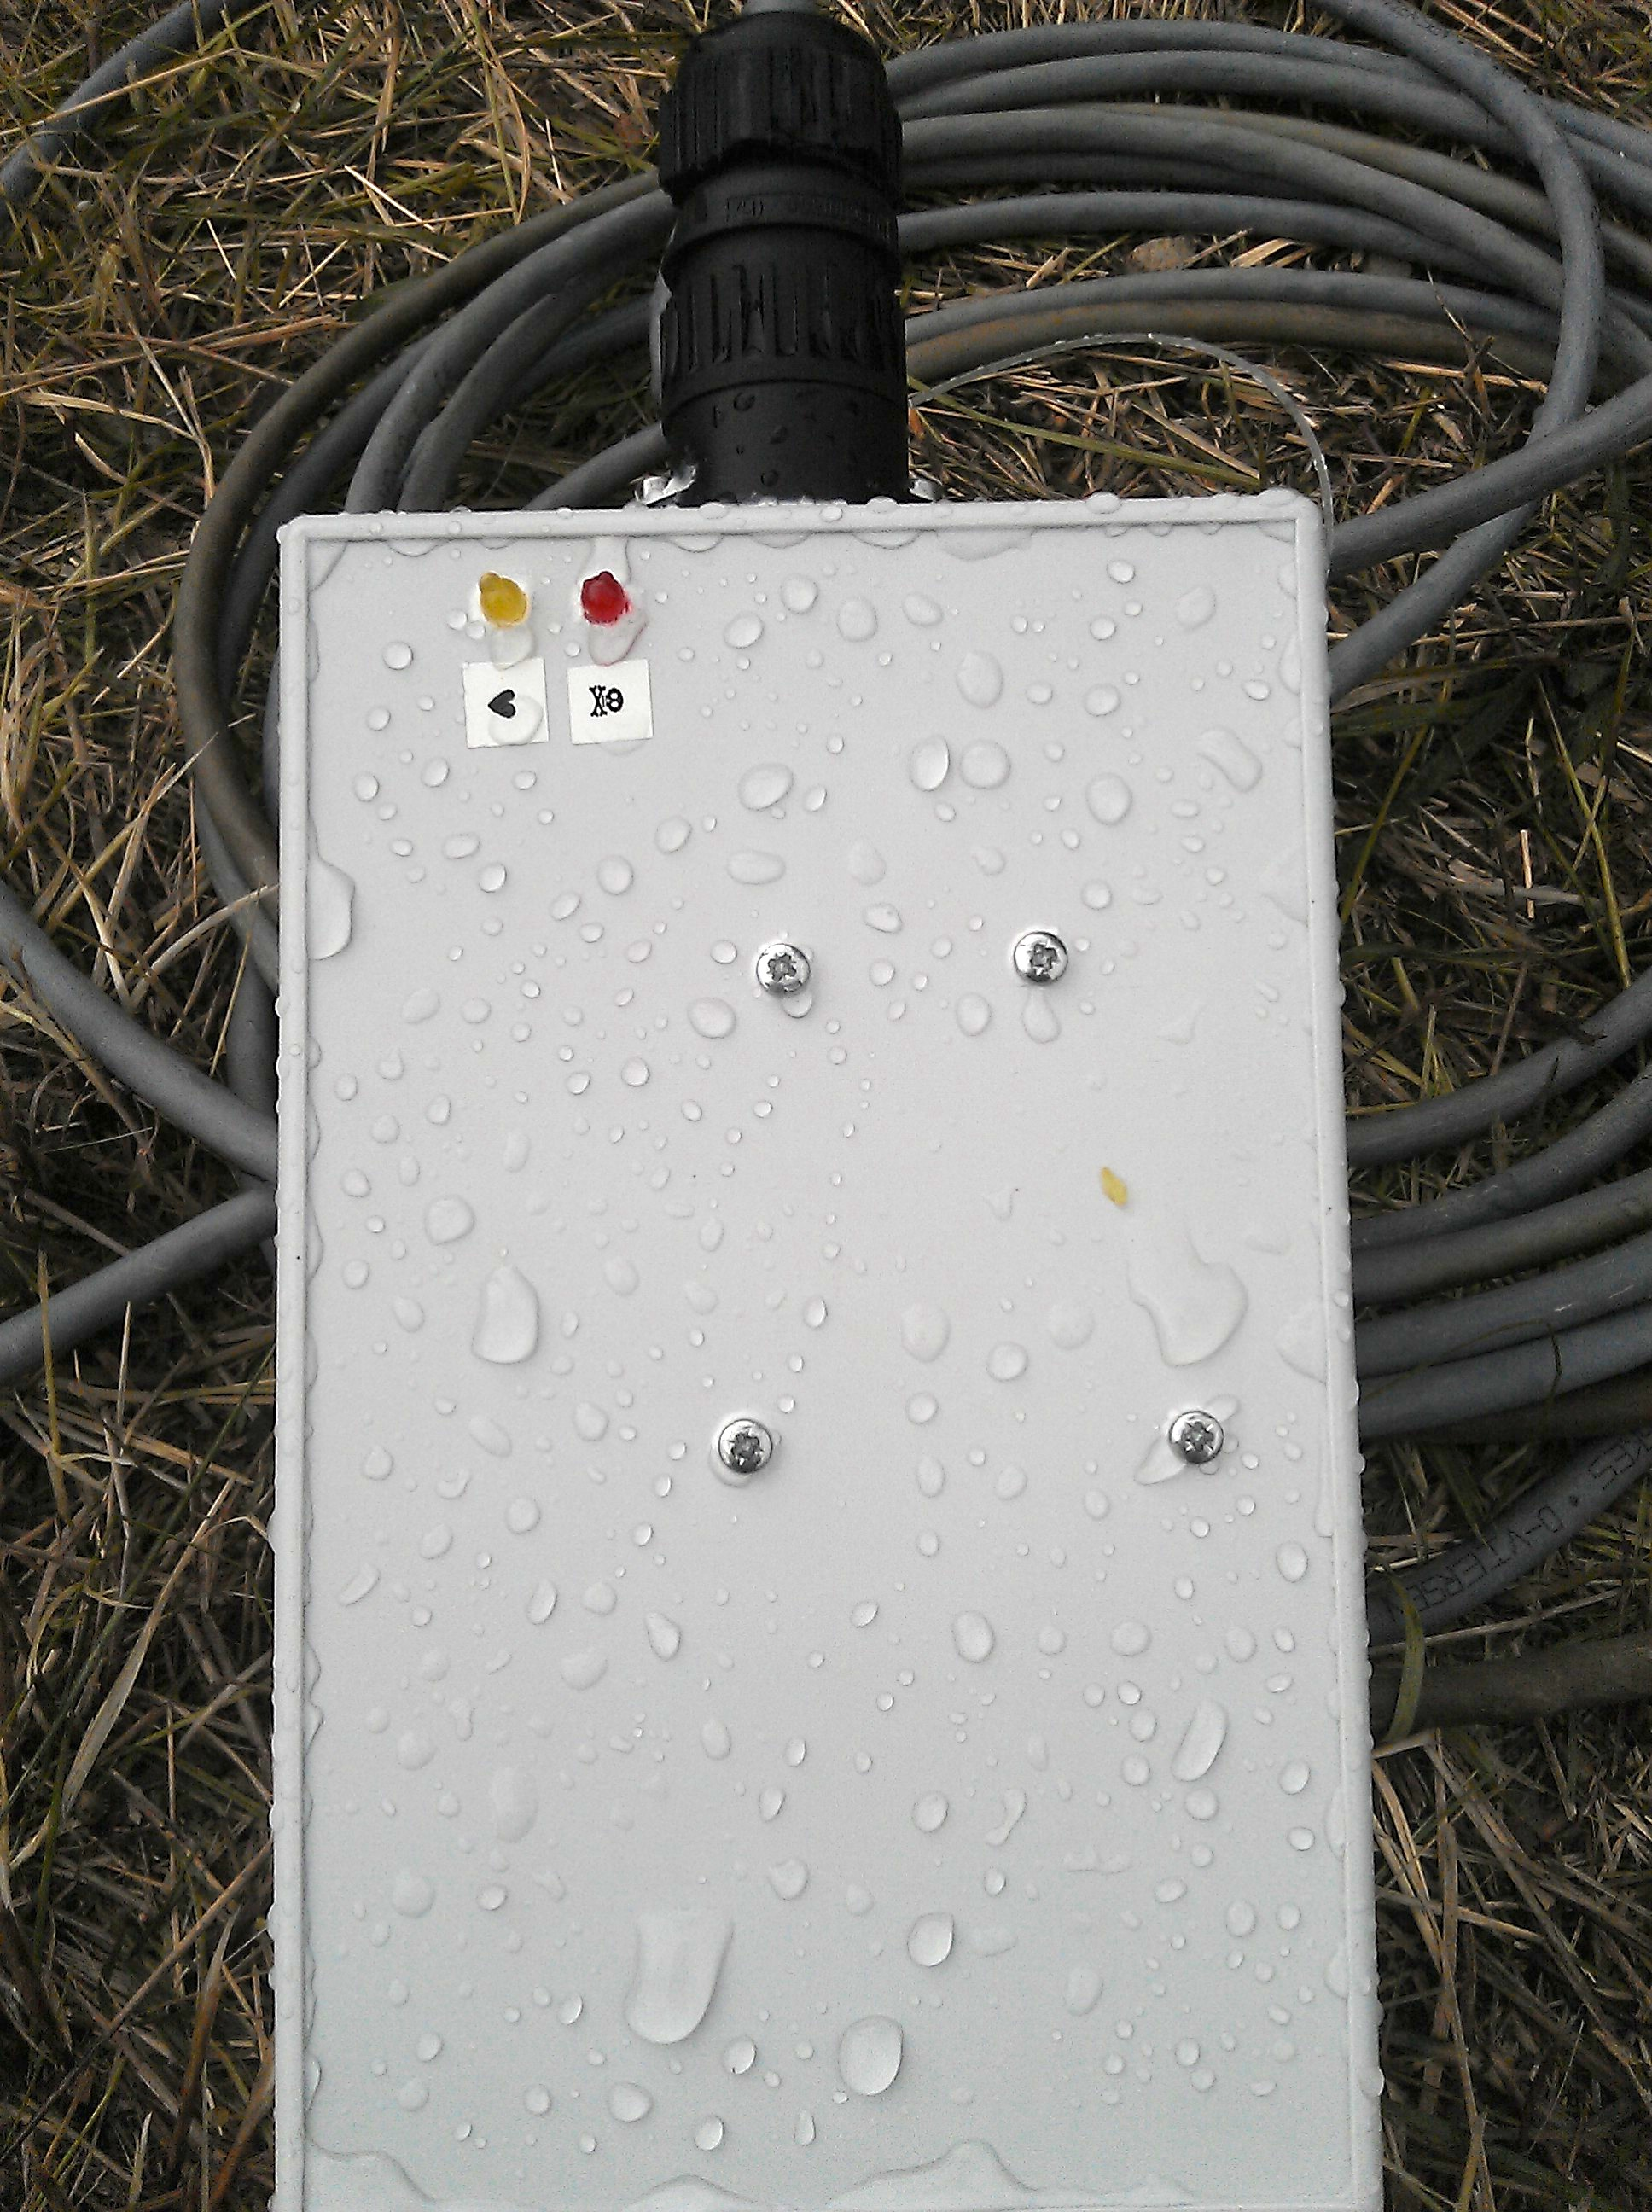
\includegraphics[width=7cm]{hardwareimages/arduinoboxregen.jpg}
 	\label{arduinoboxregen}
	}
	\caption{ABS Box mit Arduino}
	\label{arduinoboxfigure}
\end{figure}


\subsection{Software} 

Die Software besteht aus zwei Teilen: Der Code auf dem Arduino fragt die Daten vom Sensor ab und stellt sie per RS232 zur Verfügung. Der zweite Teil auf dem Logger sammelt die Messungen über den Seriellen Port und schreibt diese gemeinsam mit der jeweils aktuellen Uhrzeit in eine Datei.\\

Bei der Erläuterung des Codes möchte ich mich auf die wesentlichen Punkte beschränken. Die vollständigen Quelltexte befinden sich im Anhang.

\subsubsection{Arduino}

Der Arduino ist für die Kommunikation mit dem BMA180 über I$^2$C zuständig. Für diese Aufgabe nutze ich die Arduino Bibliothek bma180\footnote{Selbst nach ausführlicher Recherche ist es mir nicht gelungen den Originalauthor der Bibliothek zu ermitteln. Ich habe sie von John Mc Combs, welcher allerdings nicht der Ursprungsauthor ist. \\ https://bitbucket.org/johnmccombs/arduino-libraries/src/058c7101c8da/bma180 (August 2012)}. Sie enthält eine Sammlung von Lese und Schreibroutinen, die ich für meine Zwecke angepasst habe.
Hier möchte ich die einzelnen Schritte beschreiben, die notwendig sind, um eine Messung zu erhalten und diese an den Logger weiterzuleiten. \\

Die Steuerung des BMA180 erfolgt über direkte Zugriffe auf die Register. Entweder schreibt man einen neuen Wert in ein Register oder man liest ein Register aus. Es gibt fünf Arten von Registern - \texttt{test}, \texttt{control}, \texttt{image}, \texttt{status} und \texttt{data}.
Davon interessieren uns nur die \texttt{control} und die \texttt{data} Register. Weitere Informationen über die zusätzlichen Register lassen sich im Datenblatt \citep{Sensortec:2009rt} nachschlagen.

Die \texttt{control} Register dienen dazu, den Beschleunigungssensor zu steuern, vornehmlich also den Messbereich festzulegen und eventuell einen zusätzlichen digitalen Bandfilter einzustellen. Dazu müssen Werte in Register hineingeschrieben werden. Dazu geht man folgendermaßen vor:\\

\textbf{In Register schreiben}
\begin{enumerate}
	\item Übertragung initiieren (mit der Adresse des Sensors)
	\item Adresse des Registers senden, in welches wir schreiben möchten
	\item Daten senden, die wir in das Register schreiben möchten
	\item Übertragung beenden
\end{enumerate}

Da ein Register immer ein Byte (8 Bit) groß ist, finden sich oftmals verschiedene Einstellungen in einem Register um Platz zu sparen. Einen korrekten Schreibvorgang auszuführen wird dadurch komplexer. Daher möchte ich den Prozess am Beispiel der Messbereichseinstellung demonstrieren.

\begin{figure}[H]
%\centering
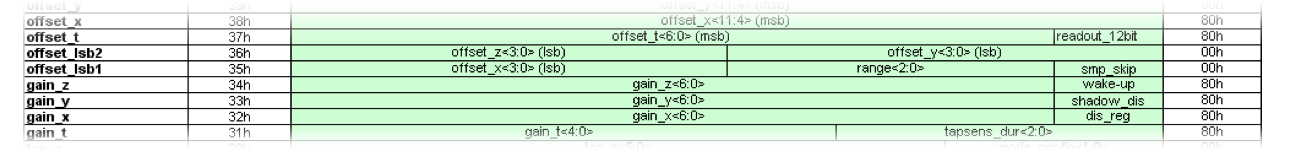
\includegraphics[scale=.359]{registerstransp}
\caption{Memory Map BMA180, Ausschnitt \citep{Sensortec:2009rt}}
\label{registermap}
\end{figure}

Die relevanten Bits befinden sich im Register \texttt{0x35}\footnote{Ein vorangestelltes \texttt{0x} bedeutet, dass es sich um eine Zahl im Hexadezimalsystem handelt}, Bit eins, zwei und drei\footnote{Es wird von rechts nach links gezählt und mit 0 begonnen} (siehe Abb. \ref{registermap} Hier die entsprechenden Zeilen aus dem Quellcode:

\lstset{language=C++,caption={Funktion zum Einstellen des Messbereichs aus der bma180 Bibliothek\\ maxg ist eine dem Wertebereich zugeordnete Binärzahl zwischen 000 und 110 },label=sensitivity}
\lstset{frameround=fttt}
\begin{lstlisting}[frame=trBL]
	void BMA180::setGSensitivty(GSENSITIVITY maxg) //1, 1.5 2 3 4 8 16
	{
	    setRegValue(0x35,maxg<<1,0xF1);
	    gSense = maxg;
	}
\end{lstlisting}
 
Die aufgerufene Funktion $setRegValue$ (Zeile 3) bekommt als Argumente das zu schreibende Register (\texttt{0x35}), den zu schreibenden Wert ($maxg << 1$) und zusätzlich eine Maske, die angibt, welche Bits des Registers nicht(!) verändert werden sollen.\\
Da das letzte Bit (Bit Null) eine andere Funktion hat, 'schieben' wir $maxg$ mit Hilfe der \textit{bitshift Operation} $<<$ um ein Bit nach links.\\
Bei $gSense$ (Zeile 4) handelt es sich um eine Statusvariable, die später benutzt wird, um den genutzten Wertebereich mit zu dokumentieren.\\


\lstset{language=C++,caption={Funktion zum Schreiben eines Registers aus der BMA180 Bibliothek},label=writeregister}
\begin{lstlisting}[frame=trBL]
	void BMA180::setRegValue(int regAdr, int val, int maskPreserve)
	{
	    int preserve=getRegValue(regAdr);	
	    int orgval=preserve & maskPreserve;
	    Wire.beginTransmission(address);
	    Wire.write(regAdr);
	    Wire.write(orgval|val);
	    int result = Wire.endTransmission();
	    checkResult(result);
	}
\end{lstlisting}

Nun lesen wir zunächst den bisherigen Wert des Registers ein (Zeile 3)  und maskieren ihn mit der übergebenen Maske, so dass wir alle Bits übernehmen, außer die, welche wir verändern wollen (Zeile 4). Dann schreiben wir in das Register, wobei wir nach dem oben beschriebenen Schema vorgehen. Beim Senden der Daten verknüpfen wir jedoch $orgval$ mittels eines bitweisen $OR$ mit dem zu schreibenden Wert (Zeile 7). So haben wir sichergestellt, dass wir nur die relevanten Bits verändern.\\
In Abbildung \ref{bitops} ist das Vorgehen noch einmal dargestellt.

\begin{figure}[H]
\centering
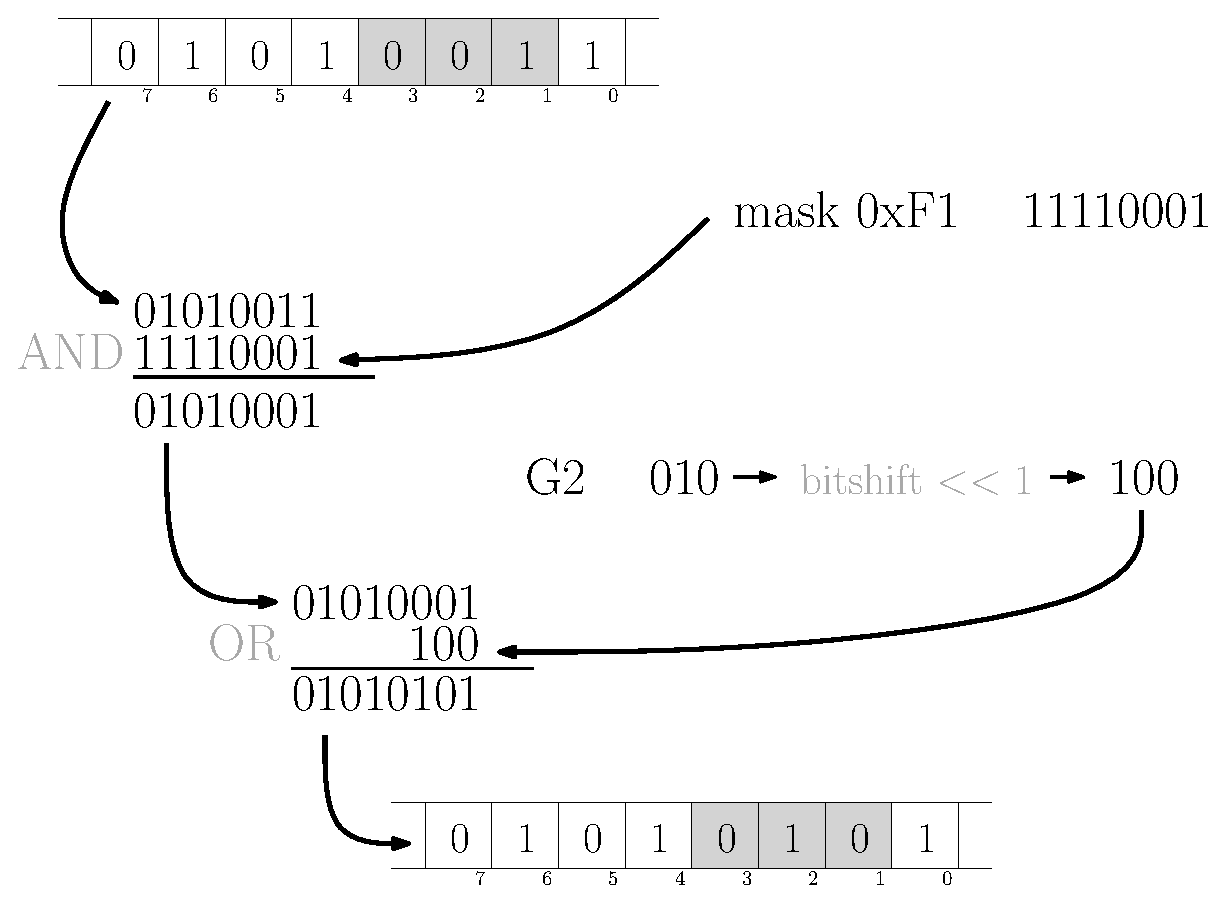
\includegraphics[scale=.5]{bitops.eps}
\caption{Beispiel eines Schreibvorgangs in das Register \texttt{0x35}. Nur die grau markierten Bits werden verändert.}
\label{bitops}
\end{figure}

\textbf{Daten aus Registern lesen}

In die data Register werden die gemessenen Beschleunigungsdaten geschrieben. Da der A/D-Wandler des BMA180 eine Auflösung von 14 Bit hat, existieren pro Achse 2 Register mit jeweils 8 Bit. 
Hier benötigen wir das Konzept der \textbf{Bitwertigkeit}:

In einer Zahl haben die Stellen unterschiedlichen Wert. Verändert man zum Beispiel bei der Zahl 4650 die letzte Stelle, so ist der Unterschied maximal 9 (4650 verglichen zu 4659). Wird hingegen die dritte Stelle (von hinten) verändert, so kann der Unterschied bis zu 900 betragen. Analog verhält es sich mit den binären Zahlen. 
Dabei bezeichnen wir das höchstwertige Bit als \textbf{m}ost-\textbf{s}ignificant-\textbf{b}it \textbf{(msb)} und das geringwertige Bit als \textbf{l}east-\textbf{s}ignificant-\textbf{b}it \textbf{(msb)}.

Analog dazu spricht man vom höchstwertigen Byte \textbf{m}ost-\textbf{s}ignificant-\textbf{b}yte \textbf{(MSB)} und geringwertigen Byte \textbf{l}east-\textbf{s}ignificant-\textbf{b}yte \textbf{(LSB)}.

\begin{equation}
\overbrace {\underbrace{1}_{msb}000101101}^{MSB}\overbrace {11010011\underbrace{0}_{lsb}}^{LSB}
\end{equation}

Die gemessene Beschleunigung ist also aufgeteilt und muss im Programm wieder zusammengesetzt werden. \\

Um die Beschleunigungsdaten vom Sensor zu laden, ist so vorzugehen:
\begin{enumerate}
	\item Übertragung initiieren (mit der Adresse des Sensors)
	\item Adresse des Registers senden, bei dem wir \textbf{anfangen} wollen zu lesen
	\item Übertragung beenden
	\item So viele Bytes abrufen, wie wir haben möchten
	\item Übertragung beenden
\end{enumerate}

\lstset{language=C++,caption={Funktion zum Auslesen der Beschleunigungsdaten, x,y,z sind 2 Byte Integerzahlen},label=readaccel}
\begin{lstlisting}[frame=trBL]
	void BMA180::readAccel()
	{
	  unsigned int result;

	  Wire.beginTransmission(address);
	  Wire.write(0x02);
	  Wire.endTransmission();
	  Wire.requestFrom((int)address, 7);
	  if(Wire.available()==7)
	  {
	    int lsb = Wire.read()>>2;
	    int msb = Wire.read();
	    x=(msb<<6)+lsb; 
	    if (x&0x2000) x|=0xc000; // set full 2 complement for neg values
	    lsb = Wire.read()>>2;
	    msb = Wire.read();
	    y=(msb<<6)+lsb;
	    if (y&0x2000) y|=0xc000;
	    lsb = Wire.read()>>2;
	    msb = Wire.read();
	    z=(msb<<6)+lsb;
	    if (z&0x2000) z|=0xc000;
	    temp = Wire.read();
	    if (temp&0x80) temp|=0xff00;
	  }
	  result = Wire.endTransmission();
	}
\end{lstlisting}

Das Register, bei dem wir beginnen wollen zu lesen, ist \texttt{0x02}, (Zeile 6) und wir benötigen die nächsten 7 Bytes (Zeile 8). Jeweils zwei Bytes MSB und LSB für die drei Achsen und als letztes Byte lesen wir zusätzlich die aktuelle Temperatur aus. Diese wird jedoch im Weiteren nicht verwendet.\\

Mit $Wire.requestFrom(adress, n)$ fordern wir einen Stapel von $n$ Bytes vom Sensor (Zeile 8). $Wire.read()$ entfernt immer das oberste Byte von diesem Stapel und gibt seinen Wert aus. Da das LSB an Stelle null und eins für den Messwert nicht relevante Bits enthält, entfernen wir diese per Bitshift (Zeile 11). Dann shiften wir das MSB im ganzen um sechs Stellen nach links, um es dann mit dem LSB zu addieren und damit den kompletten Messwert zu erhalten (Zeile 13).\\

Da die Daten im sogenannten Zweierkomplement (näheres in \citep{Tietze:2002fk}) ausgegeben werden und es sich bei x (sowie bei y und z) um Integer Variablen handelt, müssen wir das Vorzeichenbit an vorderster Stelle setzen. Dies geschieht in Zeile 14 (bzw. Zeile 18 für y und Zeile 24 für z).\\



\begin{figure}[H]
\centering
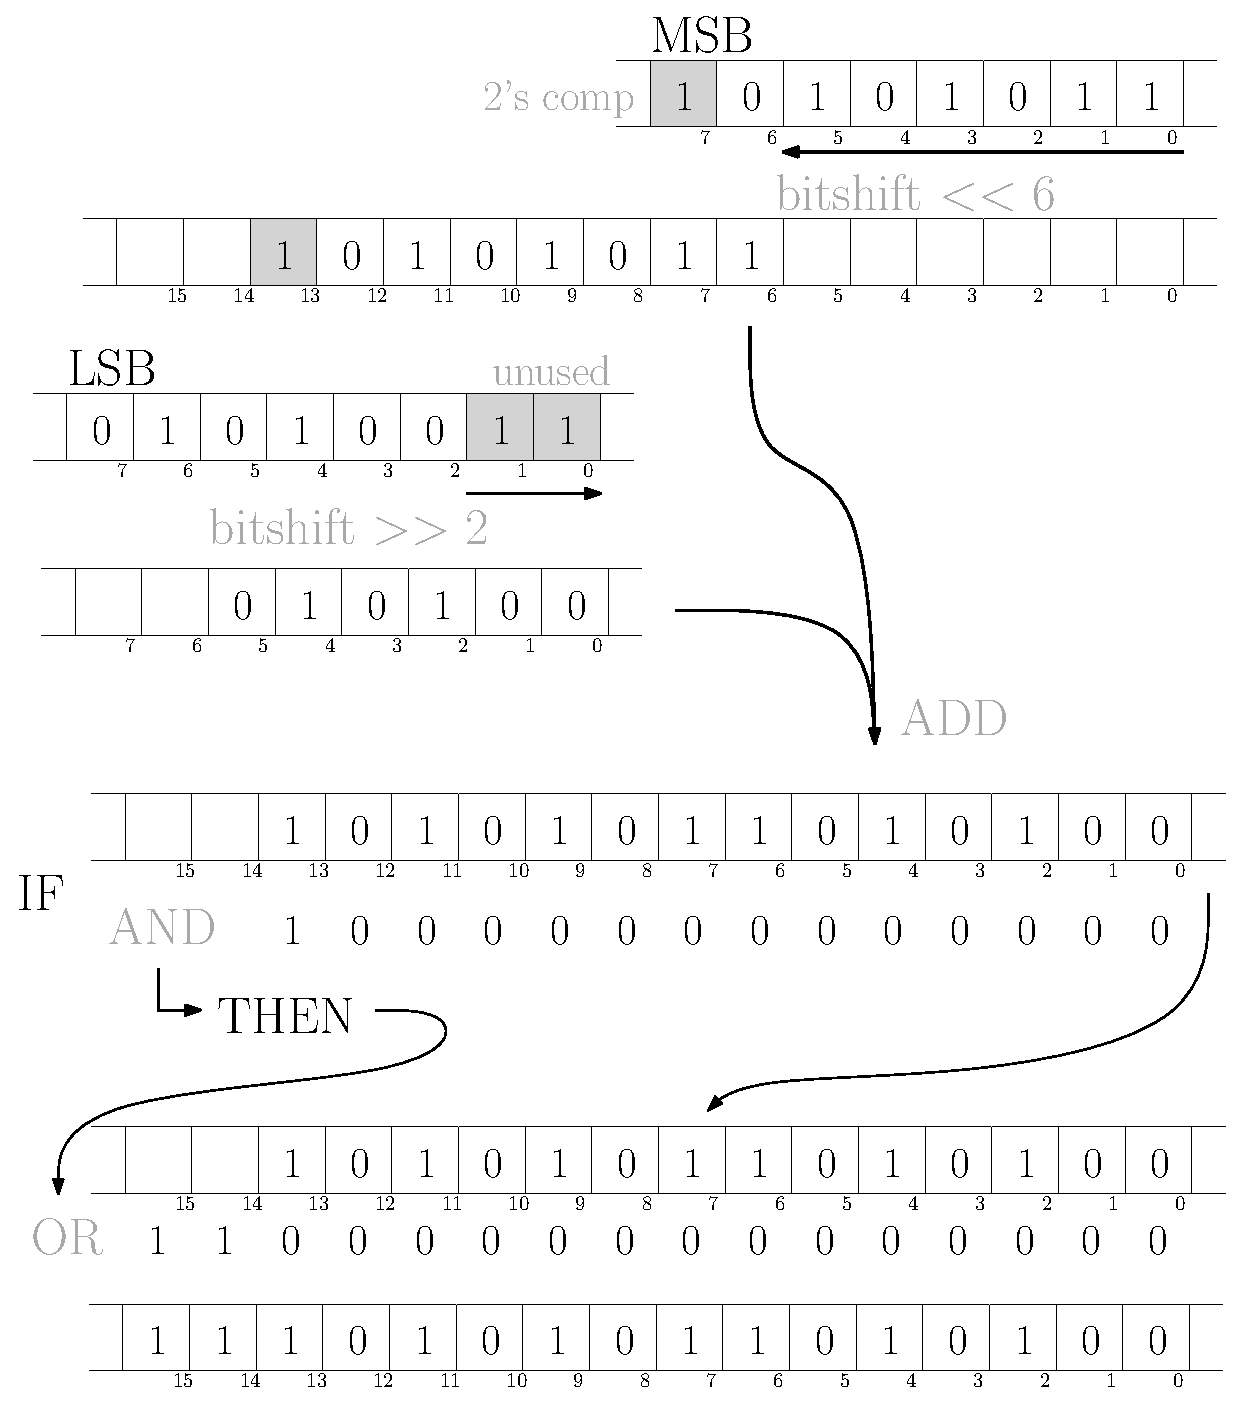
\includegraphics[scale=.55]{auslesen.eps}
\caption{Auslesen und zusammenfügen der Daten. MSB und LSB werden addiert. Mittels IF Abfrage und Masking wird überprüft, ob es sich um eine negative Zahl handelt; Falls ja, so wird das korrekte Zweierkomplement gebildet und als Integer gespeichert.}
\label{auslesen}
\end{figure}


\subsubsection{Restitution}

Jetzt haben wir eine Beschleunigungsmessung, jedoch ist diese noch in gerätespezifischen 'count' Einheiten. Diese müssen nun die physikalisch bestimmte Einheit der Beschleunigung umgerechnet werden. Der Vorgang wird als Restitution bezeichnet und der entsprechende Code ist in Listing \ref{restitution} zu sehen.

\lstset{language=C++,caption={Restitution der aufgenommenen Beschleunigungsdaten. Ausgabe als Vielfaches von der Erdbeschleunigung $g = 9.81m/s^2$},label=restitution}
\begin{lstlisting}[frame=trBL]
	float BMA180::getXValFloat()
	{
	    // normalize (if x is maximum (8191) and GSENSE=1.0 then 1.0
	    return (float)x/8191.0*getGSense();
	}
\end{lstlisting}

Aus dem Datenblatt \citep{Sensortec:2009rt} lässt sich entnehmen, dass $10~0000~0000~0000$ den geringstmöglichen Wert in jedem Messbereich darstellt und $01~1111~1111~1111$ de größten. Das erste Bit gibt dabei das Vorzeichen an (Zweierkomplement). Teilt man den Wert durch 8191, was in Binärdarstellung $1~1111~1111~1111$ entspricht, erhält man nach einer Multiplikation mit dem Messbereich (GSENSE) die Beschleunigung als Vielfaches der Erdbeschleunigung $g = 9.81 m/s^2$.


\subsubsection{PC Logger}

Das Programm, welches auf dem PC läuft und die Daten aufzeichnet, ist ein Python Script, welches ich von Matthias Hort übernommen und angepasst habe. Sobald es gestartet ist und eine kurze Beschreibung für das aktuelle Experiment eingegeben wurde, nimmt es sämtliche Nachrichten auf dem eingestellten Comport entgegen und schreibt diese mit der jeweils aktuellen Systemzeit in eine Datei.

Die exakte Zeit ist sehr wichtig, um die Ergebnisse später mit anderen Messungen vergleichen zu können. Zu diesem Zweck ist der PC mit einem NTP (Network Time Protocol) Server verbunden, welcher stets die korrekte Uhrzeit von GPS-Satelliten empfängt und im Netzwerk zur Synchronisation bereitstellt. Ein Programm auf dem PC (Domain Time II) korrigiert mit dieser GPS Zeit die computerinterne Uhr.

\newpage

\section{Berechnung der Wegwerte aus den Beschleunigungsdaten}

\subsection{Numerische Integration}

Um aus den gemessenen Beschleunigungen die gesuchten Wegwerte (Ausschläge) zu ermitteln, müssen die Messwerte zweifach über die Zeit integiert werden. Da die zu integrierenden Funktionen als begrenzte Anzahl von Abtastpunkten in diskreten Zeitabständen vorliegen, bietet es sich an, numerische Integrationsverfahren anzuwenden. Die dazu möglichen Verfahren, wie z.B. Rechteckverfahren, Trapezformel, Rombergverfahren, unterscheiden sich durch die Art der Interpolation zwischen den Abtastpunkten \citep[S. 760ff]{Bronstein:1995fk}. Die Wahl des Integrationsverfahrens beeinflusst dabei die Genauigkeit des Ergebnisses.

In dieser Arbeit verwende ich die Trapezformel und komme damit für den Weg auf folgende Rekursionsformel:

\begin{equation}
y_{i+1} = \Delta t^2 \cdot a_i - y_{i-1} + 2 \cdot y_i
\end{equation}

Mit dieser Formel kann aus den vorherigen Wegwerten $y_{i-1}$ und $y_i$ sowie den gemessenen Beschleunigungen $a_i$ und dem Zeitintervall $\Delta t$ der nächste Wegwert bestimmt werden.

Die Startwerte für $i=1$ sind vorerst nicht bekannt und können z.B. $y_0 = y_1 = 0$ gewählt werden. Dies führt allerdings zu systematischen Fehlern, die später behoben werden müssen.


\subsection{Problematik des Integrierens Noisebehafteter Daten}

Wie alle nicht synthetischen Daten enthalten die aufgenommen Beschleunigungsmessungen ein gewisses Rauschen. Schwankungen in der Spannungsversorgung, elektromagnetische Einstreuungen oder thermisches Rauschen sind einige Beispiele für mögliche Ursachen. Solange das Signal deutlich größer ist als das Rauschen, ist das kaum ein Problem. Man spricht von einem guten Signal- zu Rauschverhältnis. 

Bei der Integration der Beschleunigungswerten zu Wegwerten handelt es sich jedoch gewissermaßen um eine Addition aller Messwerte und damit einer Addition allen Rauschens. Je länger die Zeit ist, über die integiert wird, desto größer wird der Fehler in den Wegdaten. 

\begin{figure}[htb]
\centering
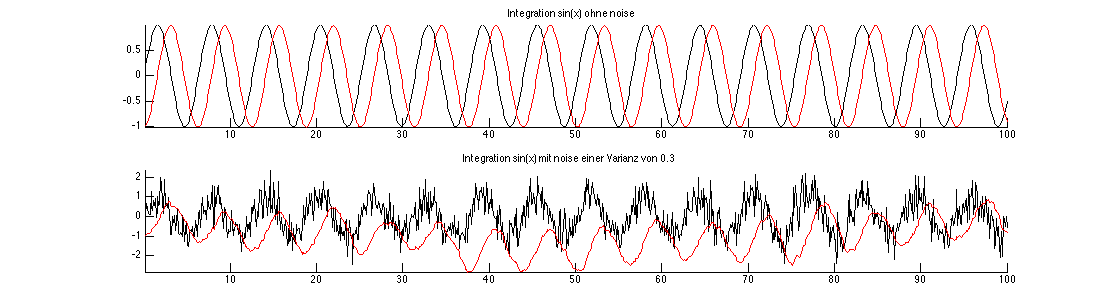
\includegraphics[scale=.4]{sinusnoise.png}
\caption{Numerische Integration von $sin(x)$. Oben: ohne Noise Unten: Mit Noise einer Varianz von 0.3}
\label{sinusnoise}
\end{figure}

Das Resultat ist in Abbildung \ref{sinusnoise} zu erkennen. Ich habe in Matlab eine Sinusfunktion mit 1000 Stützstellen numerisch integriert. Dabei habe ich zunächst keinen Noise hinzugefügt. Bei der unteren Abbildung jedoch liegt auf dem Sinus ein Rauschen mit einer Varianz von $0.3$. Es ist eine deutliche Drift der resultierenden Daten zu sehen. Bei der zweifachen Integration, die man benötigt um aus den Beschleunigungsdaten Wegdaten zu berechnen, tritt dieser Effekt sogar noch verstärkt auf. Die Fehler der Messungen überlagern die eigentlichen Messergebnisse und führen damit zu völlig falschen Wegstrecken. \\

Um diesen Effekt zu verhindern, müssen die Daten gefiltert werden. Die sich dafür bietenden Möglichkeiten möchte ich in der jeweiligen Auswertung besprechen.

\newpage

\section{Experimente in Waakirchen}

Um das System in der Anwendung zu testen, habe ich im Mai 2012 an Eruptionsdynamikexperimenten in Waakirchen, in der Nähe von München, teilgenommen. Diese Experimente wurden gemeinsam mit der Ludwig-Maximilians-Universität München, der Universität Catania und dem Istituto Nazionale di Geofisica e Vulcanologia (Sezione di Catania and Dept. of Seismology and Tectonophysics, Rome) durchgeführt. 

Bei diesen Experimenten wurden künstliche Explosionen in Autoklaven \citep{Spieler:2004fk} verschiedener Geometrie (von 16 cm bis 40 cm Länge) ausgelöst. Es kamen dabei zwei Aufbauten zum Einsatz, von denen einer das Erhitzen der Proben auf bis zu $850\circ C$ und damit der Wirklichkeit nähere Umgebungsbedingungen ermöglichte. Bei den verwendeten Samples handelte es sich um Proben von verschiedenen Vulkanen (sowohl Asche als auch festes Lavagestein) und Analogmaterialien.
Die Experimente wurden wiederholt durchgeführt und dabei potentielle Einflussgrößen wie Korngröße, Mischverhältnis, Druck und Temperatur variiert.

Untersucht wurde dabei eine Vielzahl von Parametern durch den Einsatz von Hochgeschwindigkeits- Thermo- und optischen Kameras, Piezo Sensoren, einem akustischen Array und unserem Doppler Radar.\\

Mein Ziel war dabei vor Allem, den Prototypen im Feld zu testen und Informationen über die Größenordnung der an der Radarantenne auftretenden Geschwindigkeiten zu gewinnen. Zusätzlich wollte ich die Bewegung des Autoclavenaufbaus untersuchen, um herauszufinden, ob dessen Bewegung Einfluss auf die Messungen haben kann.


%%%%%%%%%%%%%%%%%%%%%%%%%%%%%%%%%%%%%%%%%%%%%%%%%%%%%%%%%%%%%%%%
%%%%%%%%%%%%%%%%%%%%%%%%%%%%%%%%%%%%%%%%%%%%%%%%%%%%%%%%%%%%%%%%

\section{Ergebnisse der Messungen in Waakirchen}



\subsection{Messungen an der Radarantenne}

\begin{figure}[H]
\centering
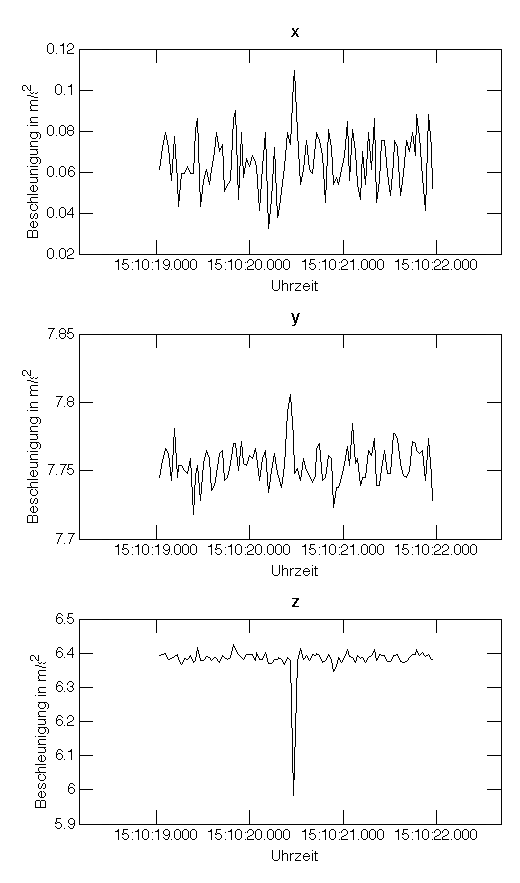
\includegraphics[scale=.5]{wakiki/firstexample2.png}
\caption{Restituierte Beschleunigungsdaten in 3 Komponenten während Experiment 7.\\ Die X-Achse entspricht der Querachse (Nickachse) des Radars, die Y-Achse seiner Hochachse und die Z-Achse der Längsachse, welche in Radarstrahlrichtung ausgerichtet ist. }
\label{firstexample}
\end{figure}

In Abbildung \ref{firstexample} sind exemplarisch die Beschleunigungsdaten aus Experiment 7 zu sehen. Es wurde mit 32 Hz aufgenommen und der Messbereich auf $\pm 1.5g$ eingestellt. {\color{red}(Auf andere verweisen? alle anhängen??)} Auf der Z-Achse ist ein deutlicher Ausschlag um ca. $0.4 m/s^2$ zu sehen, welcher durch die Druckwelle der Explosion zustande kommt. 

Die Bewegung der Schüssel wird allerdings lediglich durch ein einziges Sample erfasst. Es ist nicht sichergestellt, ob hier wirklich das Maximum an Beschleunigung abgebildet ist und wie die Bewegung genau verläuft. Eine Bestimmung der Geschwindigkeit oder des Weges durch Integration ist damit praktisch nicht möglich. 

An dieser Stelle sei auch auf das Nyquist Theorem verwiesen. Es besagt, dass ein Signal immer mindestens mit der doppelten Frequenz des hochfrequentesten Anteils im Signal abgetastet werden muss, damit es komplett rekonstruiert werden kann.  \citep[vgl.][]{Shannon:1949uq}\\

Betrachtet man lediglich das Sample, bei dem die Beschleunigung auftritt und interpoliert linear zu den nächsten beiden Samples, welche noch keine Beschleunigung anzeigen, so lässt sich dennoch eine Geschwindigkeit abschätzen. Diese ergibt sich demnach als:

\begin{equation}
v = \frac{1}{2} ~a \cdot t
\end{equation}

Im betrachteten Experiment 7 ist $v = 0.012 m/s$. Diese Geschwindigkeit ist sehr gering und kann vom Radar nicht aufgelöst werden. Aus den eben genannten Gründen ist dieses Ergebnis vorsichtig zu betrachten. Eine höhere Abtastrate ist notwendig um sicherere Aussagen treffen zu können.\\


Vergleicht man den Zeitpunkt des Maximalausschlags (15:10:20.465 Uhr) mit dem vom Radar ermittelten Explosionszeitpunkt (15:10:20.274 Uhr), so ergibt sich ein Unterschied von $191$ Millisekunden. Diese Differenz lässt sich nicht durch die langsamere Ausbreitungsgeschwindigkeit der Druckwelle erklären. Es gab offensichtlich ein Problem mit der Zeitsynchronisation, so dass das Radar nicht zu jedem Zeitpunkt eine korrekte GPS Zeit besaß. \\



{\color{red}Korrelation zwischen Geschwindigkeit (Radargemessen) und gemessener Beschleunigung? bringt mit den 3 Experimenten, wo alles gemeinsam zu sehen ist wenig... }




\subsection{Messungen am Autoklavenaufbau}


\begin{figure}[H]
\centering
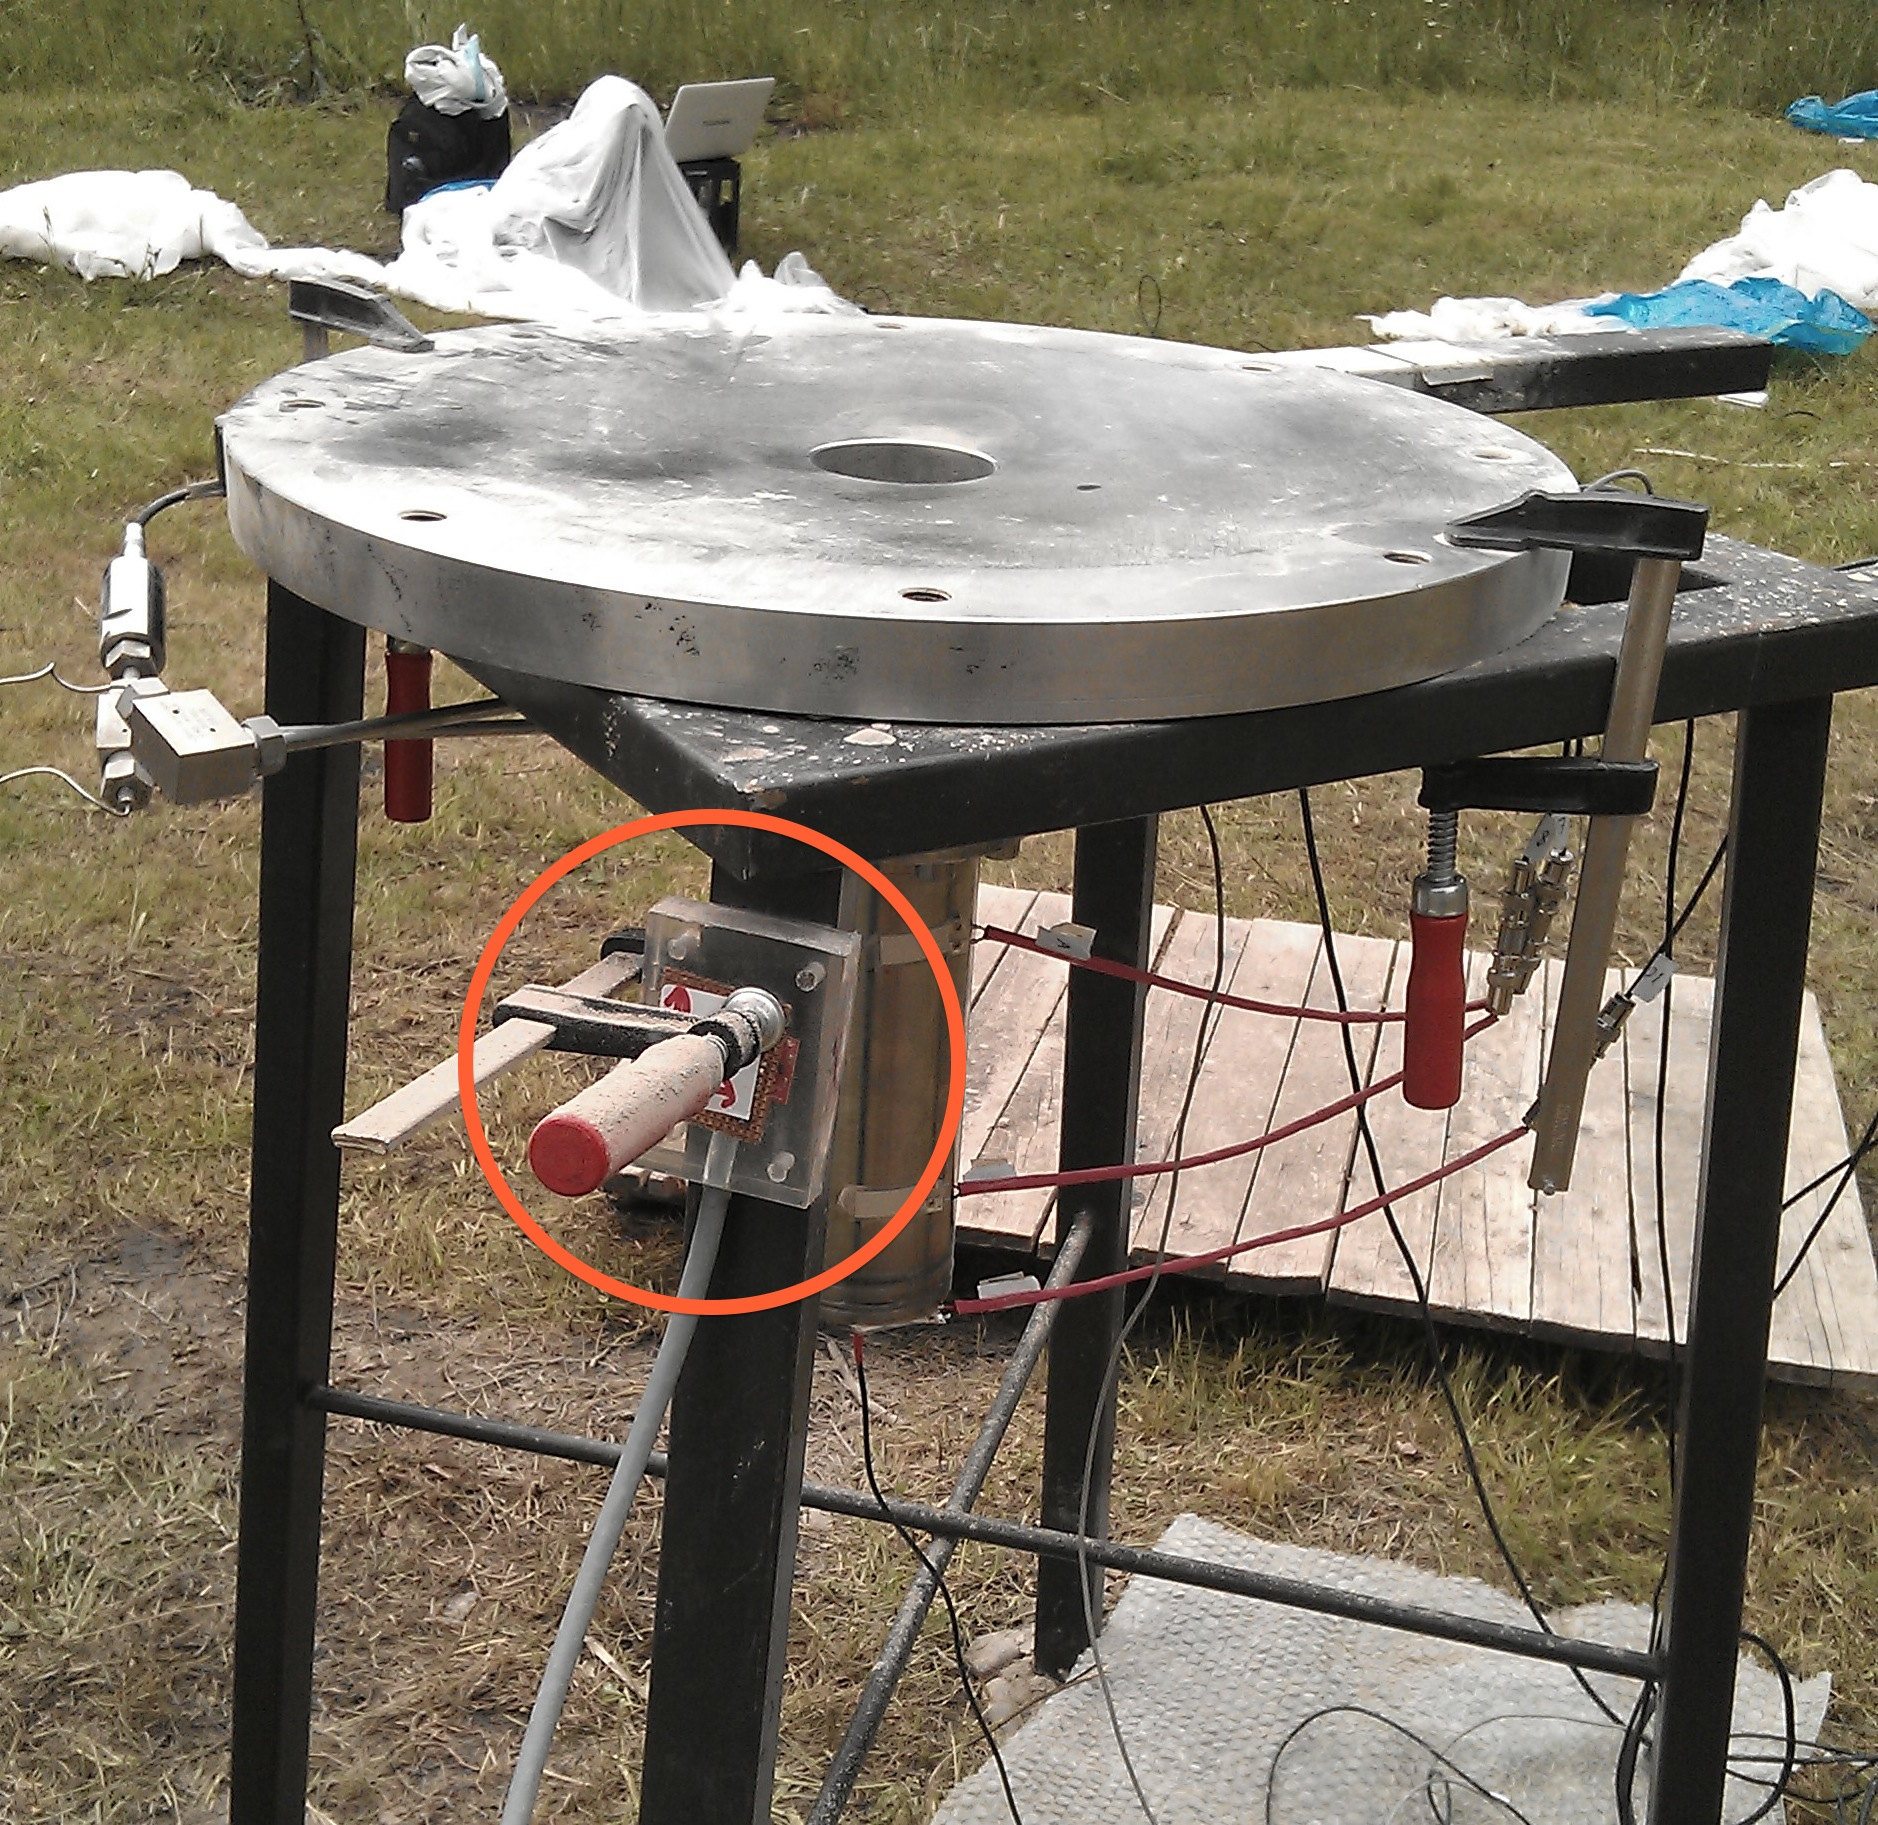
\includegraphics[scale=.13]{hardwareimages/tisch.jpg}
\caption{Messaufbau: Bewegungsmessung des Autoklavenaufbaus. Der Beschleunigungssensor ist am Bein des Aufbaus befestigt (roter Kreis).}
\label{tisch}
\end{figure}

Während Experiment 16 habe ich den Beschleunigungsmesser am Bein des Autoklavenaufbaus befestigt. Die Ausrichtung der Achsen ist in Abbildung \ref{tisch} verdeutlicht.

Es wurde wiederum mit einer Aufnahmefrequenz von 32Hz aufgezeichnet und der Messbereich war auf $\pm 4g$ eingestellt.
In Abbildung \ref{tischmovement3} sind die Ergebnisse zu sehen.\\

Zum Explosionszeitpunkt sind Beschleunigungen in allen drei Raumrichtungen zu erkennen. Der Messbereich war zu fein gewählt, die aufgetretenen Beschleunigungen sind teilweise größer als $4g$. 

Zur genaueren Betrachtung der Vertikalbewegung ist in Abbildung \ref{tischmovement_y} nur die Y-Komponente der Beschleunigung aufgetragen. 


\begin{figure}[H]
\centering
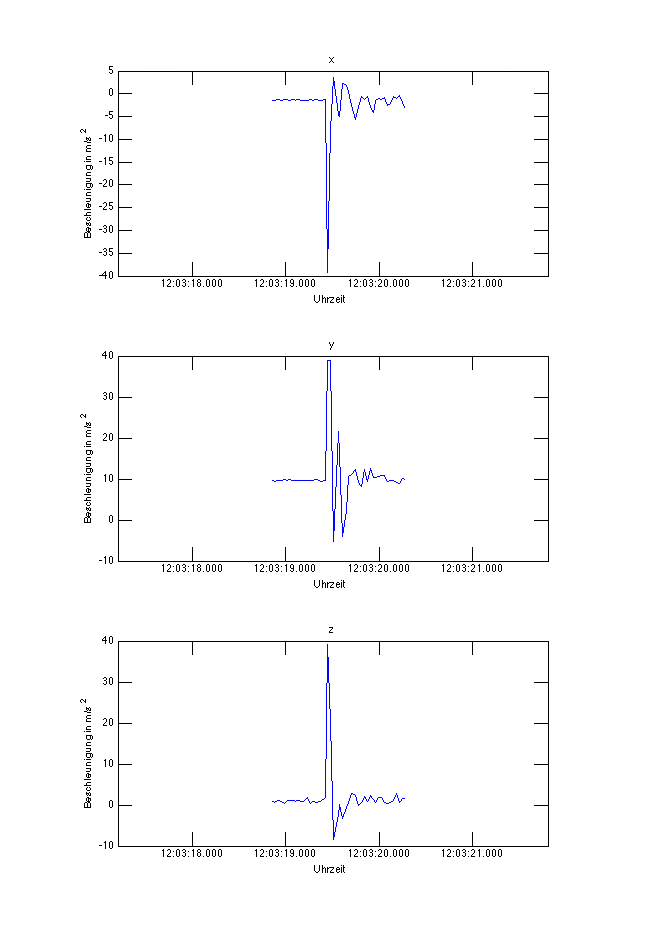
\includegraphics[scale=.5]{wakiki/tischmovement3.png}
\caption{Restituierte Beschleunigungsdaten am Autoklavenaufbau. Experiment 16. Die Ausrichtung der Achsen kann Abbildung \ref{tisch} entnommen werden. }
\label{tischmovement3}
\end{figure}

\begin{figure}[H]
\centering
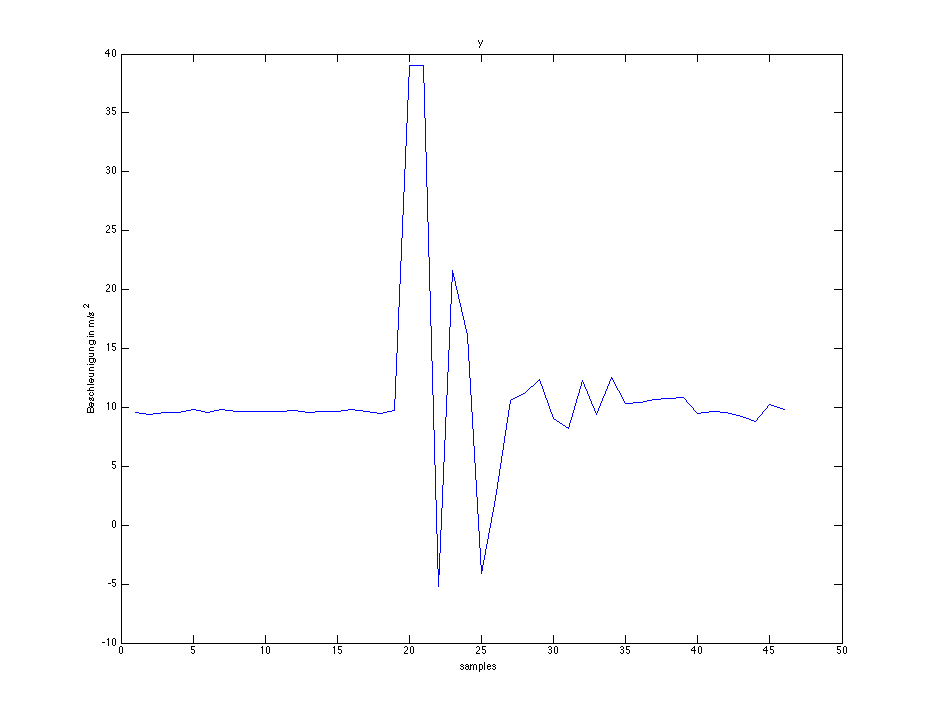
\includegraphics[scale=.4]{wakiki/tischmovement_y.png}
\caption{Y-Komponente der Beschleunigung. Der Tisch führt eine gedämpfte Schwingung aus. Deutlich erkennbar ist der zu gering gewählte Messbereich, der Erstausschlag ist nach oben hin 'abgeschnitten'}
\label{tischmovement_y}
\end{figure}

Die Messung zeigt, dass der Tisch eine gedämpfte Schwingung ausführt. Der Erstausschlag ist positiv, also bewegt sich der Tisch zunächst nach oben. Dann fällt er wieder auf den Boden zurück und schwingt ca.  eine Sekunde lang nach.

Mit der bei der Messung an der Antennenschüssel bereits angewandten Abschätzung der Geschwindigkeit erhalten wir zu Beginn eine Maximalgeschwindigkeit von ca. $1.33 m/s$. Der wahre Wert ist größer, da das Maximum der Beschleunigung nicht korrekt erfasst wurde. 



\newpage
\section{Entwicklung des Schwingungsmesssystems: ASC 5511LN-002}


Mit den bisher gewonnenen Erkenntnissen konnte ich nun das zweite Schwingungsmesssystem mit dem ASC Chip (ASC 5511LN-002) realisieren. Durch die höhere Auflösung und Samplerate und geringeres Rauschen, ergibt sich ein besser nutzbares Signal. Einen Vergleich der relevanten technischen Daten enthält Tabelle \ref{sensorcompare}.

\begin{table}[ht]
\begin{tabular}{@{}llll@{}}    
      			\cmidrule(r){1-4}\morecmidrules\cmidrule(r){1-4}
       			Beschleunigungsaufnehmer & Auflösung & Noise & Temperatur Drift\\
      			\midrule
 			BMA180 				   & 0.244 mg  & 150$\mu g / \sqrt{Hz}$ & 0.5 $mg/k$ \\ 
 			ASC 5511LN-002 		   & 0.077 mg  &    5$\mu g / \sqrt{Hz}$  & 0.2 $mg/k$\\
 		
   			\addlinespace
   			\bottomrule
 \end{tabular}
 \caption{Vergleich der relevanten technischen Daten der beiden Sensoren bezogen auf einem Messbereich von $\pm$2g.\\ Das Auflösungsvermögen des ASC 5511LN-002 bezieht sich hier auf die Verwendung mit  dem \textit{Diamond-MM-16-AT PC/104 Analog I/O Module}}
 \label{sensorcompare}
\end{table}

\subsection{ASC 5511LN-002}

\begin{figure}[H]
\centering
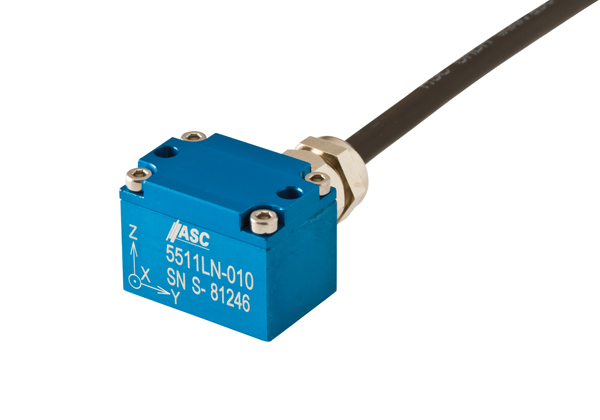
\includegraphics[scale=.5]{hardwareimages/asc.jpg}
\caption{ASC 5511LN-010 von Advanced Sensors Calibration}
\label{asc5511}
\end{figure}

Bei dem ASC 5511LN-002 handelt es sich ebenfalls um einen kapazitativen MEMS Sensor. Er ist allerdings von hochwertigerer Qualität als der BMA180 und gibt das Signal analog als Spannung aus. Aus diesem Grund wird ein externer AD-Wandler benötigt.
Durch das Aluminiumgehäuse ist die Elektronik bereits gut geschützt und die symmetrische Ausführung der Signalkabel sorgt dafür, dass äußere elektromagnetische Einflüsse auf dem Weg zum AD-Wandler vermieden werden. Das Signal wird als auf zwei Leitungen ausgegeben, wobei das Signal auf der einen Leitung invertiert ist (Abb. \ref{symmetrisch}). Störungen wirken auf beide Adern und somit kann man sie an der Empfangsstation per Differenzbildung leicht entfernen. 
\begin{figure}[H]
\centering
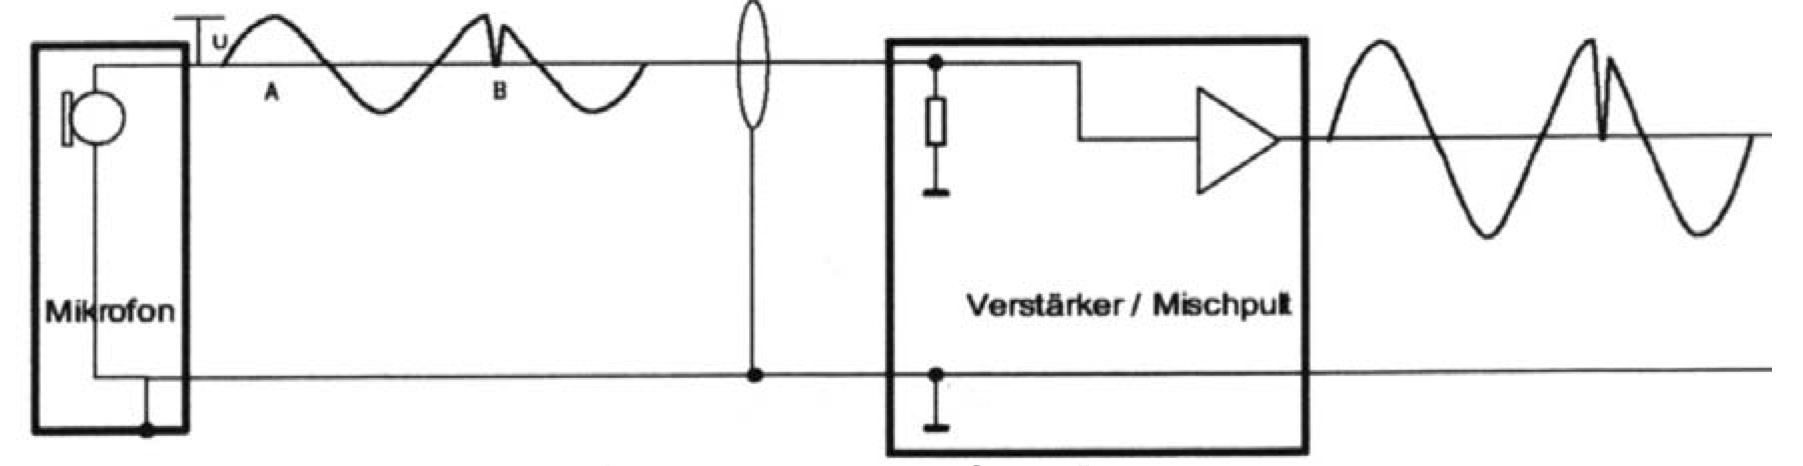
\includegraphics[scale=.7]{unsymmetrisch.png}
\caption{Unsymmetrische Signalübertragung mit Störung 'Zacke'. \citep{Sengpiel:2001fk}}
\label{unsymmetrisch}
\end{figure}


Bei unsymmetrischer Signalführung wird das Störsignal ebenso stark verstärkt, wie das Nutzsignal (Abb. \ref{unsymmetrisch}). Mathematisch lässt sich dies so ausdrücken \citep{Sengpiel:2001fk}:

\begin{equation}
U_a = v \cdot (U_e + U_{stoer} = v \cdot U_e + v \cdot U_{stoer}
\end{equation}

wobei $U_a$ dem Ausgangssignal, $U_e$ dem Eingangssignal, $U_stoer$ dem Störsignal und $v$ dem Verstärkungsfaktor entspricht.

\begin{figure}[H]
\centering
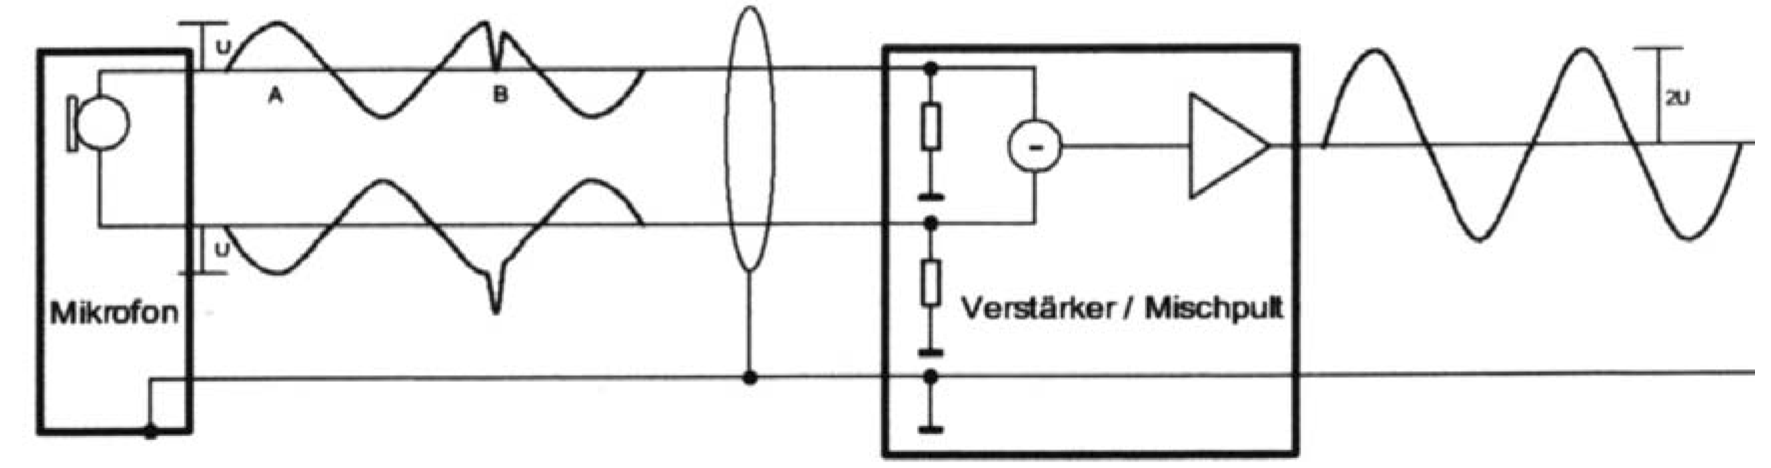
\includegraphics[scale=.7]{symmetrisch.png}
\caption{Symmetrische Signalübertragung mit sich aufhebender Störung. \citep{Sengpiel:2001fk}}
\label{symmetrisch}
\end{figure}

Symmetrische Signalführung hingegen sorgt dafür, dass sich der Störeinfluss auslöscht:

\begin{equation}
U_a = U_e + U_{stoer} - ( -U_e + U_{stoer} ) = 2 \cdot U_e
\end{equation}

Das Resultat ist ein besseres Signal zu Rausch Verhältnis.


\subsection{Diamond-MM-16-AT PC/104 Analog I/O Module}

\begin{figure}[H]
\centering
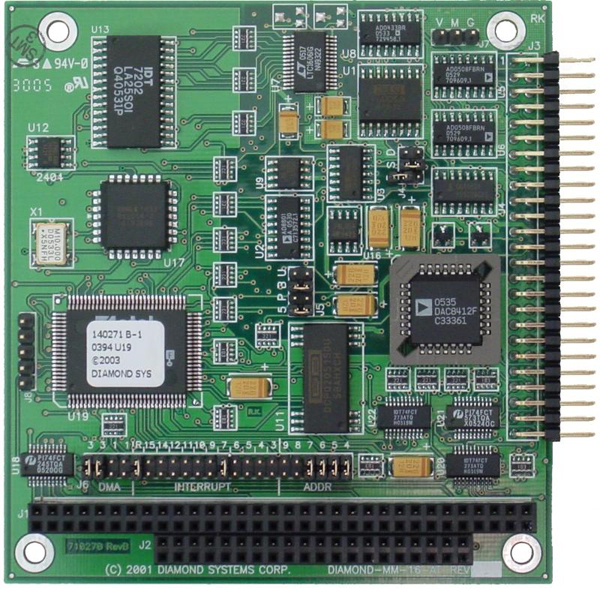
\includegraphics[scale=.4]{hardwareimages/diamondmm16at.jpg}
\caption{Diamond-MM-16-AT PC/104 Analog I/O Module}
\label{diamond}
\end{figure}



Als AD-Wandler verwende ich ein \textit{Diamond-MM-16-AT PC/104 Analog I/O Module}. Das Board verfügt über 8 Eingänge (16 wenn man sie nicht als Differentialeingänge verwendet) und eine maximale Samplingrate von 100kHz. Außerdem besitzt es einen 512-Sample \textit{FIFO Speicher} und verwendet \textit{Interrupts}, worauf ich in den beiden nächsten Punkten eingehen möchte.
Mit dem Computer kommunizert das Board über den \textit{PC/104 Bus}.


\subsubsection{Interrupts}

\begin{figure}[H]
\centering
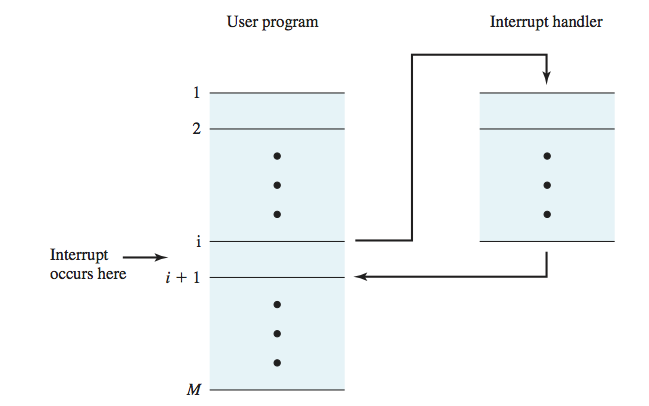
\includegraphics[scale=1.4]{interrupt.png}
\caption{Ablauf eines Interrupts \citep{Stallings:2000uq}}
\label{interrupt}
\end{figure}

Ein Interrupt beschreibt in der Informatik eine kurzzeitige Unterbrechung des normalen Programmflusses, um eine andere Operation auszuführen. Diese andere Operation ist Zeitkritisch und ihr exaktes Auftreten nicht vorher bestimmbar. Sobald sie beendet ist, setzt das Programm seine Ausführung an der vorher unterbrochenen Stelle fort.

Genutzt werden Interrupts zum Beispiel von Ein- und Ausgabegeräten, wie Maus und Tastatur. Ohne Interrupts müssten alle Programme zyklisch nachfragen, ob es eine neue Eingabe gibt und diese dann entsprechend bearbeiten (sogenanntes Polling). Da ein Programm in dieser Zeit nichts anderes machen kann, ist diese Art der Abfrage höchst ineffizient.

Die am weitesten verbreitete Analogie zur Verdeutlichung des Prinzips ist eine Wohnungstür mit Klingel. Man kann den ganzen Tag in der Wohnung seinen Aufgaben nachgehen und zwischendurch klingeln Gäste, mit denen man sich dann kurz beschäftigt. Das klingeln ist hier also der Interrupt. Dann kann man wieder weiter mit der Arbeit machen bis der nächste klingelt. Hat man nun aber keine Klingel, so muss man ständig zur Tür rennen und nachsehen, ob eventuell jemand dort steht und gerne hereinkommen möchte (Polling).

An dieser Analogie kann man auch erkennen, dass Interrupts zusätzliche Hardware (eine Klingel) erfordern.


\subsubsection{FIFO Speicher}

\begin{figure}[H]
\centering
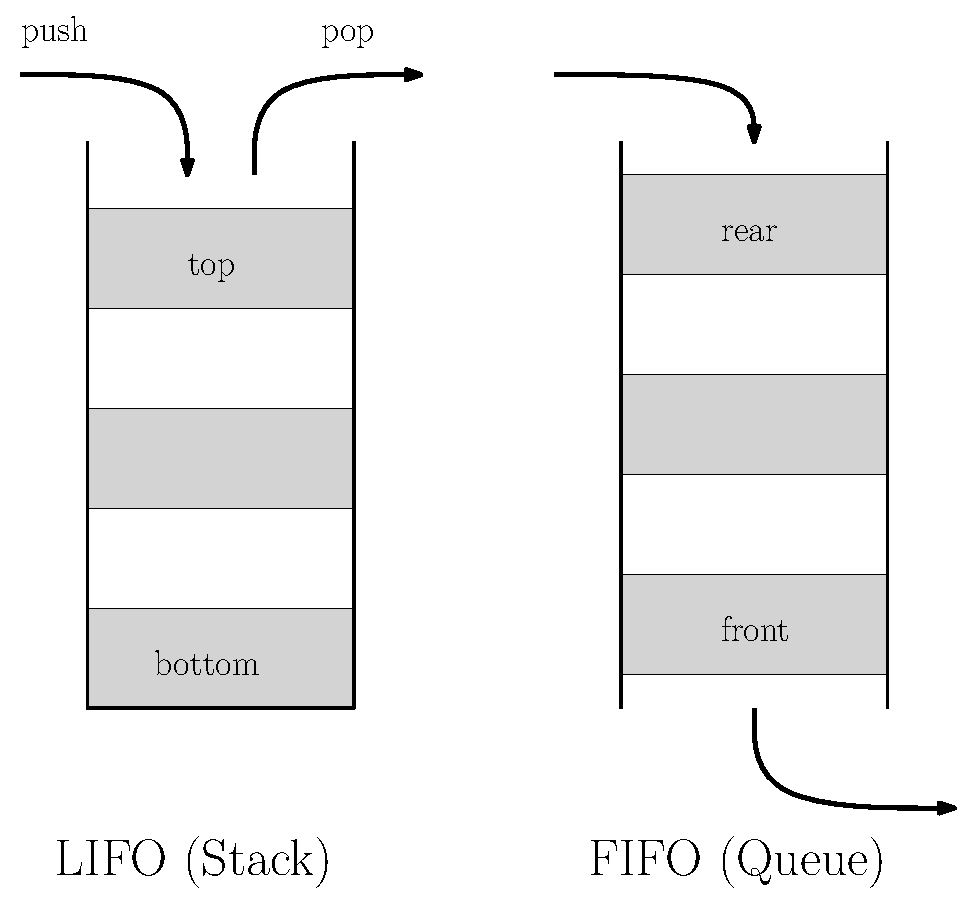
\includegraphics[scale=.7]{fifolifo.eps}
\caption{Vergleich von FIFO und LIFO}
\label{fifolifo}
\end{figure}

Ein FIFO (First In First Out) ist ein Speicherverfahren, bei dem die Elemente, die als erstes gespeichert werden, auch als erstes wieder entnommen werden. Es wird auch als Warteschlangenprinzip (Queue) bezeichnet und in vielen Bereichen der Datenverarbeitung verwendet. Besonders bei Schnittstellen und Kommunikationsprotokollen ist es wichtig, dass die Daten in der Reihenfolge verarbeiten werden, in der sie angekommen sind, beziehungsweise abgesendet wurden. Das gegensätzliche Prinzip ist das LIFO (Last In First Out), auch Stapelprinzip (engl. Stack) genannt.\\

Im AD-Wandler sorgt der FIFO dafür, dass wirklich alle digitalisierten Samples vom Computer gespeichert werden, auch wenn dieser aufgrund von starker Prozesserbelastung nicht in der Lage ist diese sofort zu verarbeiten. Die digitalisierten Daten werden unabhängig vom PC immer sofort in den FIFO gespeichert und können dort angefordert werden. Ein Problem ergibt sich erst wenn der PC die Sample so langsam ausliest, dass der FIFO Speicher voll wird. In diesem Fall spricht man von einem Speicherüberlauf und bereits aufgenommene Daten werden überschrieben.\\


Zusammen mit Interrupts erlaubt der FIFO Speicher eine konstante Messwertdigitalisierung mit hoher Frequenz, ohne den Prozessor des PCs zu stark zu beanspruchen. Dazu werden die Daten kontinuierlich vom Board in den FIFO geschrieben und sobald ein festgelegter Grenzwert (threshold) erreicht ist, löst es einen Interrupt aus. Darauf reagiert nun der PC, indem er das komplette Datenpaket auf einmal (also so viele Samples, wie der threshold Wert eingestellt ist) aus dem FIFO liest und auf seine Festplatte speichert. Währenddessen werden weiterhin Daten digitalisiert und es geht kein Sample verloren.

Würde bei jedem neuen Sample ein Interrupt ausgelöst werden und die Daten jedes Mal einzeln abgerufen und gespeichert, so würde dies bei hohen Abtastfrequenzen zu extremer Prozessorbelastung führen. Der FIFO dient also gleichzeitig auch zur Verringerung der Interrupt Rate:

\begin{equation}
Interrupt ~Rate = \frac{A/D ~Frequenz \cdot Anzahl ~der ~aufgenommenen ~Kanaele}{FIFO ~threshold}
\end{equation}

Bei einem Kanal und einer Abtastfrequenz von $100000 Hz$ resultiert, bei einem threshold von 256, ein Unterschied von $100000$ zu ca. $391$ Interrupts pro Sekunde.


\subsection{Software}

Für das Diamond Board existiert die \textit{Universal Driver Software}\footnote{http://www.diamondsystems.com/products/dscud}, eine C-basierte Programmbibliothek, die eine große Zahl von Funktionen zur Datenaquisition zur Verfügung stellt. Die Low-Level-Programmierung, bei der auf die einzelnen Register zugegriffen wird, entfällt damit. 

Bei der Entwicklung habe ich mich an der \textit{DSCADScanInt} Demo\footnote{http://files.diamondsystems.com/cdrom/Software/Universal\%20Driver/Demos/DMM16-AT\_5.91\_Demo.zip (September 2012)} aus den Beispielen der Treibersoftware orientiert.

Ich möchte wiederum nur die wichtigsten Teile des Quellcodes erläutern. Der komplette Code findet sich im Anhang. \\

Das Programm wird mit zwei Parametern aufgerufen: Dem Namen des Logfiles, in das die Daten geschrieben werden und der Anzahl an Samples, die aufgenommen werden sollen. 

Wenn im folgenden von einem Buffer gesprochen wird, so ist damit nicht der FIFO gemeint, sondern ein Speicher, in dem die Samples gespeichert werden, sobald sie aus dem FIFO herauskommen. Dieser Buffer wird nur von Interrupts beschrieben, daher wird zusätzliche Logik benötigt, um die Daten in der richtigen Reihenfolge aus diesem Buffer auszulesen. \\

Der Programmablauf ist folgendermaßen gegliedert:

\begin{enumerate}
	\item Initialisierung des Treibers
	\item Initialisierung des Boards (mit Bus-Adresse und Interrupt Level)
	\item Konfigurationsvariablen für den AD-Wandler setzen
	\item Konfigurieren des Interrupts und des FIFOs
	\item Loop, der alle x Sekunden überprüft, ob neue Daten vorliegen
		\begin{itemize}
			\item Daten in der richtigen Reihenfolge aus dem Buffer lesen und samt Zeitstempel in eine Datei schreiben
		\end{itemize}
\end{enumerate}




\textbf{Initialisierung des Treibers}

In Listing \ref{initdriver} wird zunächst der Treiber für das Board initialisiert, dabei wird überprüft, ob die korrekte Treiberversion installiert ist.
\lstset{language=C++,caption={Initialisierung der Treibersoftware},label=initdriver}
\begin{lstlisting}[frame=trBL]
	if( dscInit( DSC_VERSION ) != DE_NONE )
	{
		dscGetLastError(&errparams);
		fprintf( stderr, "dscInit error: %s %s\n", dscGetErrorString(errparams.ErrCode), errparams.errstring );
		return 0;
	}
\end{lstlisting}


\textbf{Initialisierung des Boards}

Als nächstes wird das Board selbst initialisiert (Lst. \ref{initboard}). Dazu notwendig sind die Bus-Adresse (Zeile 3) und das Interrupt-Level (Zeile 4), die auf dem Board per Jumper eingestellt werden können. Es ist dadruch möglich mehrere Boards gleichzeitig in einem Computer zu betreiben.

\lstset{language=C++,caption={Initialisierung des Boards},label=initboard}
\begin{lstlisting}[frame=trBL]
	printf( "\nDMM16AT BOARD INITIALIZATION:\n" );

	dsccb.base_address = 0x300;
	dsccb.int_level = (BYTE) 7;

	if(dscInitBoard(DSC_DMM16AT, &dsccb, &dscb)!= DE_NONE)
	{
		dscGetLastError(&errparams);
		fprintf( stderr, "dscInitBoard error: %s %s\n", dscGetErrorString(errparams.ErrCode), errparams.errstring );
		return 0;
	}
\end{lstlisting}

Der Ablauf der Konfiguration ist in allen Punkten einheitlich. Zunächst werden die entsprechenden Werte in eine Struktur geschrieben, dann wird diese als ganzes an das Board übergeben. Sollten dabei Fehler auftreten, so werden diese ausgegeben und das Programm bricht ab. \\

\textbf{Setzen der Konfigurationsvariablen für den AD-Wandler}

Der AD-Wandler kann in verschiedenen Messbereichen arbeiten und außerdem eine gewisse Signalverstärkung (gain) vornehmen. Die dazu notwendigen Einstellungen sind in Listing \ref{initad} aufgeführt. 
Der \textit{ASC 5511LN-002} gibt eine maximale Spannung von 5V aus, daher ist \texttt{RANGE\_5} der richtige Eintrag. In unserem Fall muss die Spannung auch nicht verstärkt werden. 

Über eine längere Zeit und vor allem mit der Änderung der Temperatur neigen AD-Wandler dazu, eine gewisse Drift aufzuweisen. Dies liegt daran, dass sich der Ohmsche Widerstand, welcher als Referenz zur gemessenen Spannung dient, mit der Temperatur ändert. Das \textit{Diamond-MM-16-AT} verfügt über einen Autokalibrationsmechanismus. Indem es vorher exakt bekannte Ohmsche Widerstände misst und die Messungen mit den bekannten Werten vergleicht, kann die genaue Drift bestimmt und herausgerechnet werden\citep[siehe auch][]{Miller:2006fk}.

Ob diese Autokalibration genutzt werden soll, legt \texttt{load\_cal} in Zeile 4 fest.

Zeile 5 setzt den aktuellen Kanal, bei dem die Digitalisierung beginnen soll fest.

\lstset{language=C++,caption={Konfigurieren des AD-Wandlers},label=initad}
\begin{lstlisting}[frame=trBL]
	dscadsettings.range = RANGE_5;
	dscadsettings.polarity = UNIPOLAR;
	dscadsettings.gain = GAIN_1;
	dscadsettings.load_cal = (BYTE)TRUE;
	dscadsettings.current_channel = 0;
\end{lstlisting}


\textbf{Konfigurieren des Interrupts und des FIFOs}

An dieser Stelle (Lst. \ref{initint}) wird festgelegt, dass der FIFO benutzt werden soll (Zeile 9) und wie groß der treshold ist, bei dem ein Interrupt ausgelöst wird (Zeile 11). Die Größe des FIFOs (\texttt{fifo\_depth}) ist durch die Hardware auf 256 Byte festgelegt.

\texttt{Low\_channel} (Zeile 5) und \texttt{high\_channel} (Zeile 6) geben an, welche der 8 Eingänge des Boards genutzt werden sollen. Obwohl der Beschleunigungssensor nur 3 Komponenten hat, verwende ich hier 4 Kanäle, da dies die Ausleselogik vereinfacht.

In Zeile 2 wird die Samplingrate festgelegt. Sie ist immer auf alle Kanäle bezogen, so dass sich bei einer Samplingfrequenz von 1000 Hz und 4 Kanälen eine letztendliche Abtastrate von 250 Mal pro Sekunde pro Kanal ergibt. 

Theoretisch lassen sich mit dem Board Samplingraten von bis zu 100 000 Mal pro Sekunde erreichen. Dazu ist jedoch eine genaue Kalibrierung aller Parameter und weitere Codeoptimierung notwendig, was nicht mehr Teil dieser Arbeit sein soll. \\


\lstset{language=C++,caption={Setzen der Variablen für den Interrupt},label=initint}
\begin{lstlisting}[frame=trBL]
	dscaioint.num_conversions = num_conversions;
	dscaioint.conversion_rate = 1000;
	dscaioint.cycle = (BYTE)TRUE;
	dscaioint.internal_clock = (BYTE)TRUE;
	dscaioint.low_channel = 0;
	dscaioint.high_channel = 3;
	dscaioint.external_gate_enable = (BYTE)FALSE;
	dscaioint.internal_clock_gate = (BYTE)FALSE;
	dscaioint.fifo_enab = (BYTE)TRUE;
	dscaioint.fifo_depth = 256;
	dscaioint.dump_threshold = 256;
\end{lstlisting}

In Zeile 3 lässt sich zwischen \textit{One-Shot-Mode} und \textit{Recycle-Mode} wechseln. Im One-Shot-Mode wird ein Buffer ein Mal mit Daten gefüllt und danach beendet sich die Routine. \texttt{Num\_conversions} gibt dabei die Größe des Buffers an, und damit wie viele Samples aufgenommen werden sollen.

Im Recycle-Mode wird bei Erreichen des Bufferendes zum Anfang des Buffers gesprungen und dort die alten Daten überschrieben. Der Parameter \texttt{num\_conversions} gibt in diesem Fall die Größe des Buffers an. Somit enthält dieser immer die letzten $n$ Samples, wobei $n$ die Buffergröße ist.

Um herauszufinden, an welcher Stelle im Buffer grade geschrieben wurde, dienen die beiden Variablen \texttt{DSCS.transfers} und \texttt{DSCS.total\_transfers}. \texttt{DSCS.transfers} gibt an, wie viele Samples im aktuellen Zyklus bereits im Buffer gespeichert wurden und wird immer auf 0 gesetzt wenn ein neuer Zyklus beginnt. \texttt{DSCS.total\_transfers} gibt die Gesamtzahl an bisher digitalisierter Werte in der gesamten Operation an.

Damit ist es möglich, die Daten in der korrekten Reihenfolge in eine Datei zu speichern.\\

Die weiteren in Listing \ref{initint} aufgeführten Variablen sind für unseren Anwendungsfall nicht relevant.\\


\textbf{Auslesen und Speichern der Daten}


Wie bereits beschrieben verläuft das Speichern der neuen Samples in den zirkulären Buffer automatisch durch die Interrupts. Sobald der \texttt{dump\_treshold} erreicht ist, werden die Daten vom FIFO in den Buffer übertragen. Um sie von dort aus in eine Datei zu schreiben, bedienen wir uns einer Programmschleife, die mehrmals pro Sekunde überprüft, ob neue Samples vorliegen (Lst. \ref{loop}). 

\lstset{language=C++,caption={Programmschleife, die den Buffer auf neue Daten überprüft und diese in eine Datei schreibt. Der Code zum Auslesen und Schreiben der Samples ist in diesem Listing entfernt und seperat in Listing \ref{placedafter} und \ref{placedbefore} abgebildet.},label=loop}
\begin{lstlisting}[frame=trBL]
	DWORD sleep_ms = 300;
	
	do {
        dscSleep(sleep_ms);
        dscGetStatus(dscb, &dscs);

        if ( dscs.overflows ) {
            printf("Operation failed: FIFO overflowed\n");
            break;
        }

        if ( dscs.total_transfers == last_total_transfers ) {
            printf("Operation failed: no new samples taken in %d ms\n", sleep_ms);
            break;
        }

        new_sample_count = dscs.total_transfers - last_total_transfers;

        /* Number of new samples should never exceed the size of the circular buffer.  If it does it means that either "sleep_ms" should be smaller so you check status more often, or "num_conversions" should be bigger so the circular buffer is bigger */
        if ( new_sample_count > num_conversions ) {
            printf("Operation failed: not processing data fast enough.  %d samples lost\n",
                new_sample_count - num_conversions);
            break;
        }

		/* AUSLESEN UND SPEICHERN DER DATEN  */
		/* FOLGT IM NAECHSTEN LISTING */
       
        last_transfers = dscs.transfers;
        last_total_transfers = dscs.total_transfers;

        if ( dscs.total_transfers >= stop_after_transfers )
            break;

    } while ( dscs.op_type != OP_TYPE_NONE );

    dscCancelOp(dscb);
\end{lstlisting}	

In Zeile 1 wird mit \texttt{sleep\_ms = 300} festgelegt, dass die Schleife ca. 3 Mal pro Sekunde ausgeführt wird. Zunächst wird überprüft, ob der FIFO übergelaufen ist (Zeile 7), es überhaupt neue Samples seit des letzten Schleifendurchlaufs gab (Zeile 12) und ob die Daten rechtzeitig aus dem Buffer in eine Datei geschrieben wurden (Zeile 17 und 20). 

Schlägt einer dieser Checks fehl, so wird das Programm mit einer entsprechenden Fehlermeldung beendet.\\

Treten keine Fehler auf, werden die Daten aus dem zirkulären Buffer herausgelesen und in eine Datei gespeichert.
Dies geschiet so lange, bis die Zahl der aufzunehmenden Samples erreicht ist (Zeile 32 und 33).

Da der Buffer zirkulär ist, also beim Erreichen des Endes wieder vom Anfang beschrieben wird, gibt es zwei Möglichkeiten wo die neuen Daten darin gespeichert wurden. Im einfachen Fall befinden sie sich zwischen der zuletzt ausgelesenen Position und dem Bufferende. Dieser Fall wird der Code in Listing \ref{placedafter} ausgeführt. 

\lstset{language=C++,caption={Auslesen und Speichern der Daten. Fall 1: Im zirkulären Buffer wurden neue Samples nur zwischen der zuletzt ausgelesenen Position und dem Ende des Speichers geschrieben.},label=placedafter}
\begin{lstlisting}[frame=trBL]
	if ( dscs.transfers > last_transfers ) {
		for ( i = last_transfers; i < dscs.transfers; i++ ) {
			if ( i%4 == 0 ) {
				uhr = mvTime::Now();  // get actual time
				for ( k = 0; k < 3; k++ ) { // conversion into volts
					dscADCodeToVoltage(dscb, dscadsettings, dscaioint.sample_values[i+k], &voltage[k]);
				}
					fprintf(logFile,"%s counts: %5d %5d %5d  Volts: %5.3lf %5.3lf %5.3lf\n",uhr.GetTimeStamp().c_str(),dscaioint.sample_values[i],dscaioint.sample_values[i+1], dscaioint.sample_values[i+2],voltage[0],voltage[1],voltage[2]);
			}
\end{lstlisting}		

In Zeile 1 findet die Überprüfung statt, ob die aktuelle Position im Buffer (\texttt{dscs.transfers} größer ist als die zuletzt ausgelesene Position \texttt{last\_transfers} (Also Fall 1 eingetreten ist). 
Um die nächsten Zeilen zu verstehen, ist es wichtig zu wissen, wie die einzelnen Samples im Buffer strukturiert sind. Abbildung \ref{samplebuffer} zeigt diese Struktur. 

\begin{figure}[H]
\centering
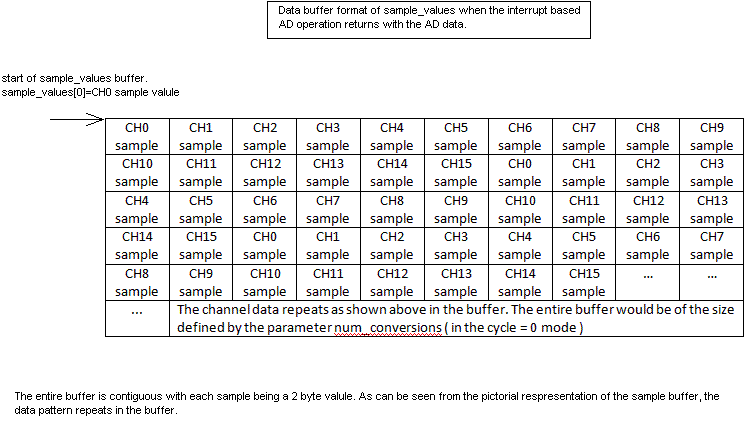
\includegraphics[scale=.55]{samplebuffer.png}
\caption{Struktur des Buffers, in dem die Samples stehen. \citep{Systems:2008uq}}
\label{samplebuffer}
\end{figure}

Alle Kanäle werden hintereinander gespeichert. Um diese nun nach Kanal sortiert auszugeben, nutze ich in Zeile 3 den Modulo Operator damit $i$ immer Kanal 0 enthält und die anderen Kanäle mit $i+1$ und $i+2$ auszulesen sind.

Die Werte müssen noch von AD-Counts mittels der Funktion \texttt{dscADCodeToVoltage} in Volt umgewandelt werden (Zeilen 5 bis 7).

Das Schreiben in eine Datei findet in Zeile 8 statt. Dabei werden sowohl die umgewandelten Voltzahlen als auch die ursprünglichen Counts gespeichert und mit einem Zeitstempel versehen. \\

Im zweiten Fall wurden neue Daten sowohl nach der zuletzt ausgelesenen Position geschrieben, als auch wieder an den Anfang des Buffers. Fall 2 ist in Listing \ref{placedbefore} zu sehen und beinahe identisch mit Fall 1. 

Es gibt allerdings zwei for Schleifen. Die erste liest Samples, die nach der zuletzt gelesenen Position gespeichert wurden (Zeile 2) und die zweite liest die Samples, welche sich zwischen dem Anfang und der aktuellen Position befinden (Zeile 10).
					
\lstset{language=C++,caption={Auslesen und Speichern der Daten. Fall 2: Im zirkulären Buffer wurden neue Samples zwischen der zuletzt ausgelesenen Position und dem Ende und zusätzlich am Anfang des Speichers geschrieben.},label=placedbefore}
\begin{lstlisting}[frame=trBL]				
	} else if ( dscs.transfers <= last_transfers ) {
		for ( i = last_transfers; i < num_conversions; i++ ) // after the last_transfers
				if ( i%4 == 0 ) {
					uhr = mvTime::Now();    // get actual time
					for ( k = 0; k < 3; k++ ) {  // conversion into volts
						dscADCodeToVoltage(dscb, dscadsettings, dscaioint.sample_values[i+k], &voltage[k]);
					}
					fprintf(logFile,"%s counts: %5d %5d %5d  Volts: %5.3lf %5.3lf %5.3lf \n",uhr.GetTimeStamp().c_str(),dscaioint.sample_values[i],dscaioint.sample_values[i+1], dscaioint.sample_values[i+2],voltage[0],voltage[1],voltage[2]);
				}
            for ( i = 0; i < dscs.transfers; i++ ) // in between beginning and last transfers
				if ( i%4 == 0 ) {
					uhr = mvTime::Now();   // get actual time
					for ( k = 0; k < 3; k++ ) { // conversion into volts
						dscADCodeToVoltage(dscb, dscadsettings, dscaioint.sample_values[i+k], &voltage[k]);
					}
					fprintf(logFile,"%s counts: %5d %5d %5d  Volts: %5.3lf %5.3lf %5.3lf \n",uhr.GetTimeStamp().c_str(),dscaioint.sample_values[i],dscaioint.sample_values[i+1], dscaioint.sample_values[i+2],voltage[0],voltage[1],voltage[2]);
				}
        }
\end{lstlisting}

Die Zeitstempel erhalte ich durch eine eine Methode aus der \texttt{mvTime} Klasse. Diese stammt aus der Radarserver Software von Malte Vöge. \\

Der Nachteil bei dieser Art der Datenaufnahme ist, dass ein neuer Zeitstempel nur bei jedem Schleifendurchlauf (drei Mal pro Sekunde) entsteht. Es haben daher immer mehrere Samples den gleichen Zeitstempel. In der Auswertung muss also zunächst ein neuer Zeitstempel generiert werden.

\newpage

\section{Experimente am Geomatikum}

\begin{figure}[htb]
\centering
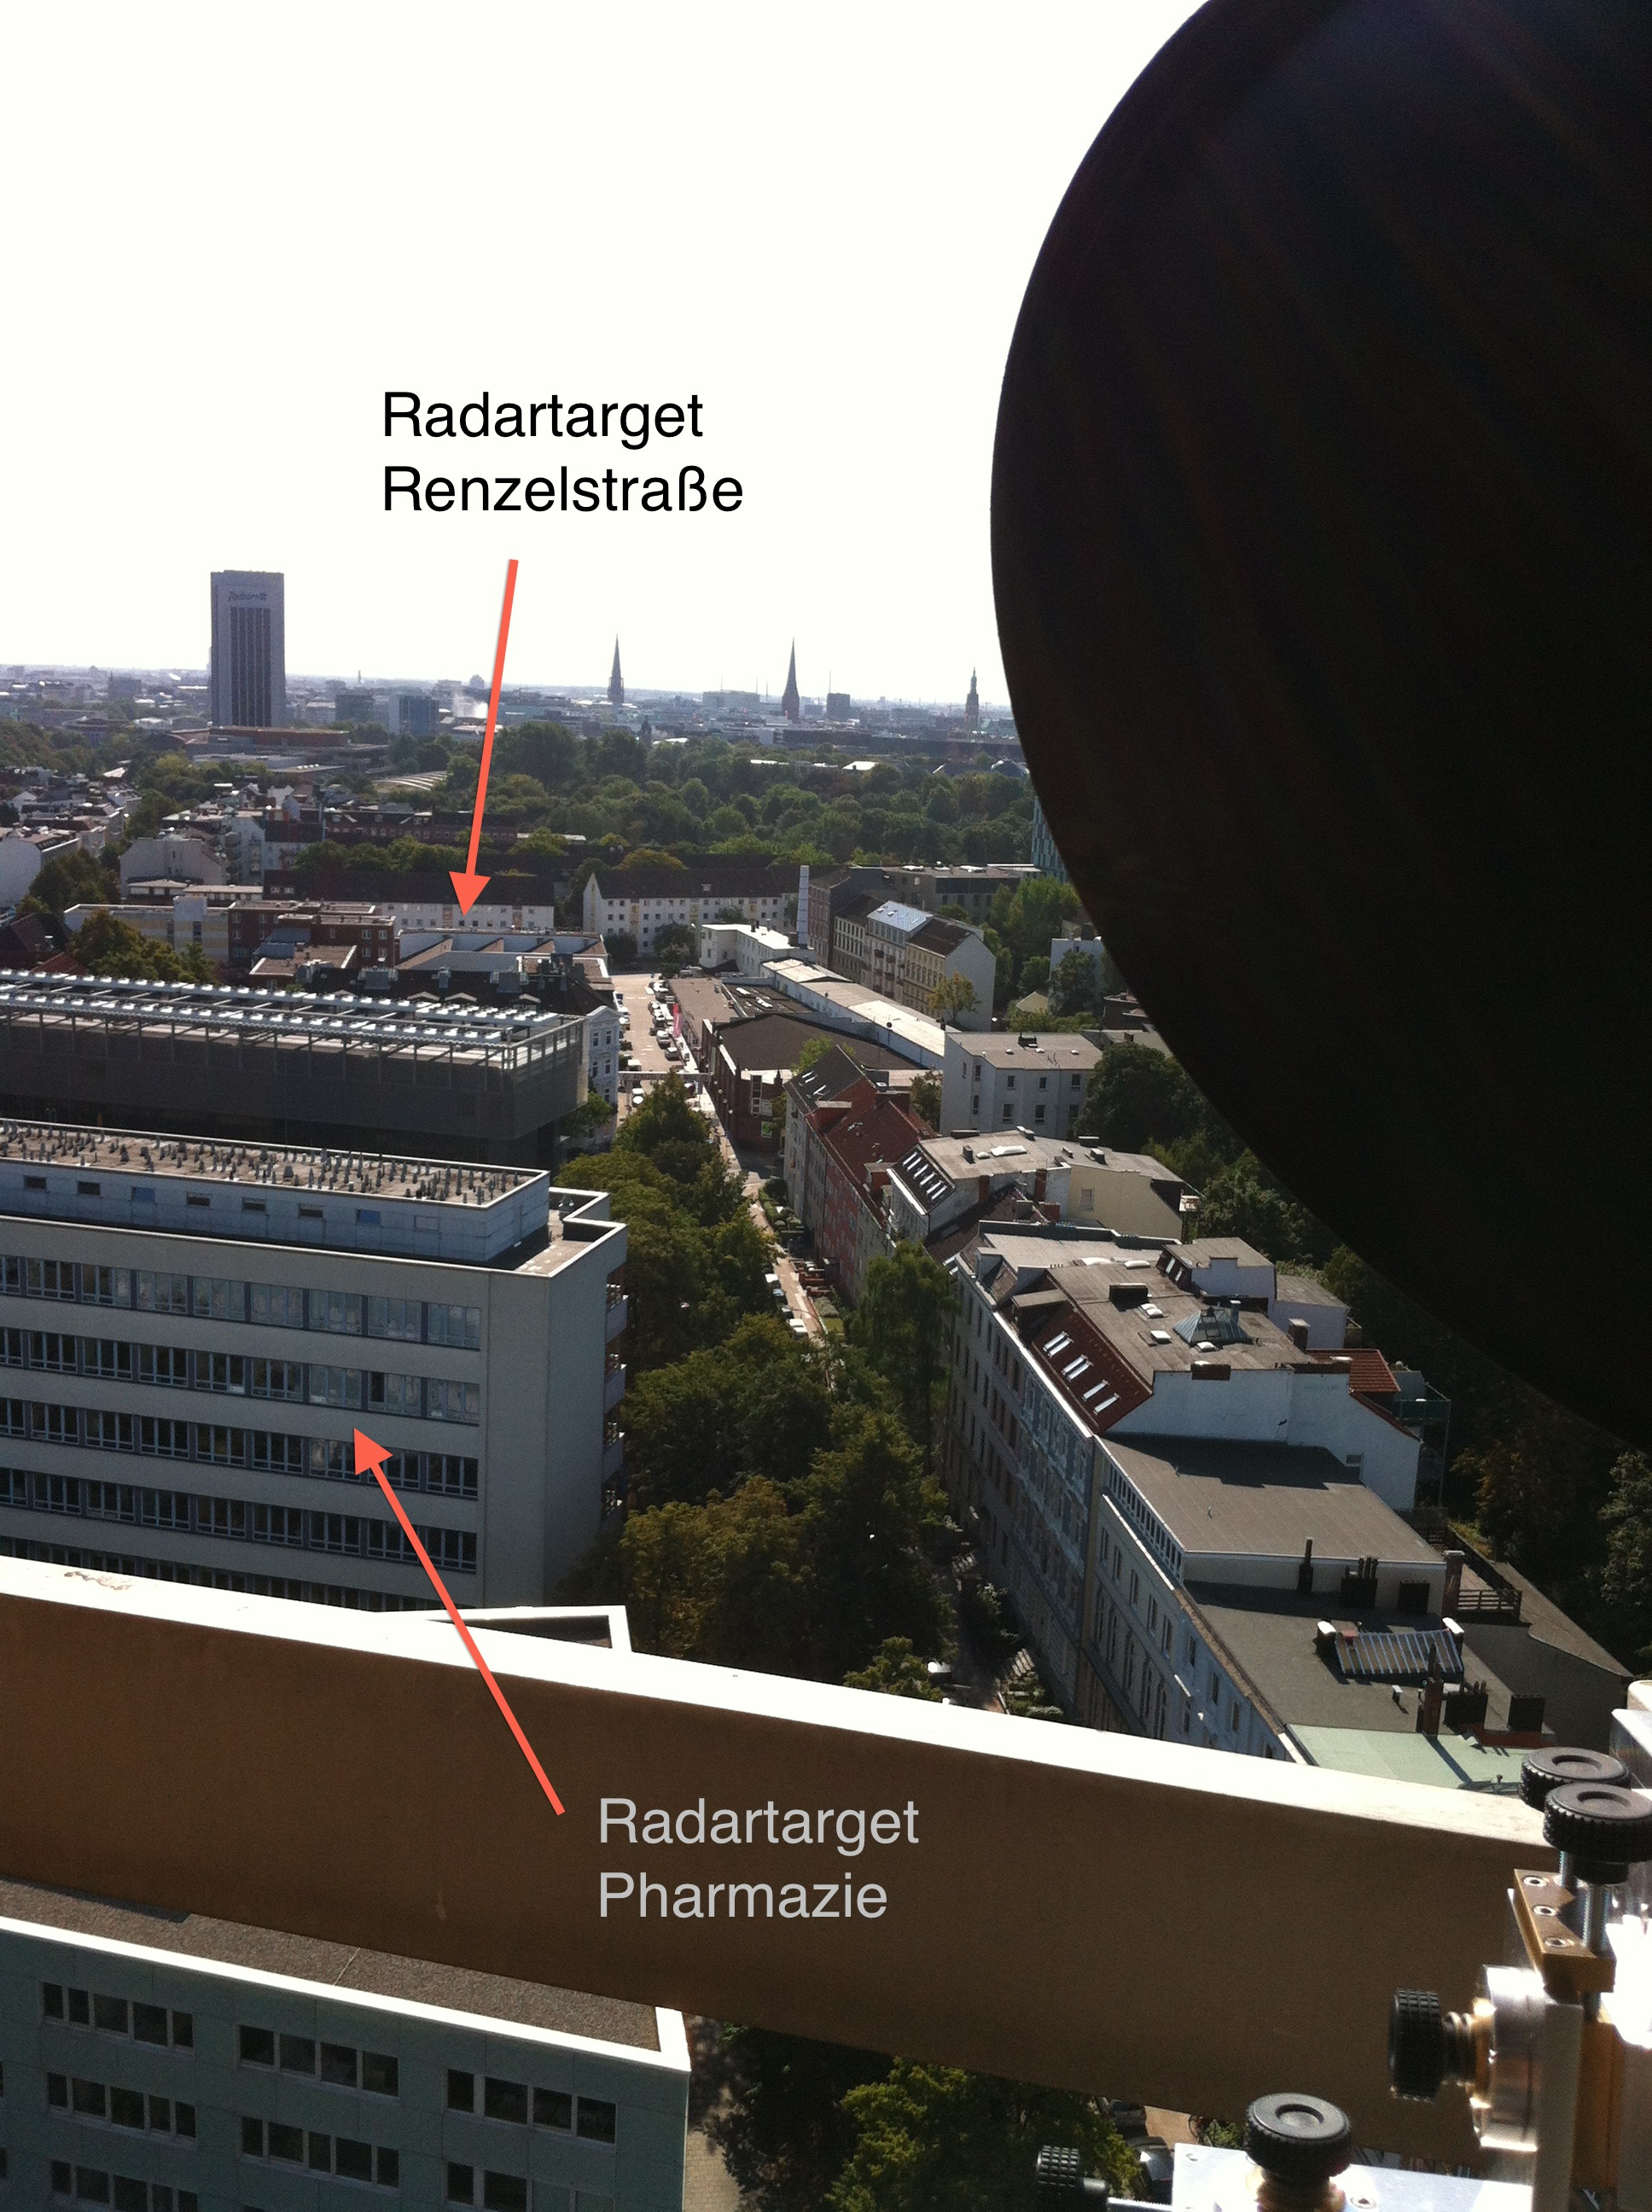
\includegraphics[scale=.13]{targets.jpg}
\caption{Ausrichtung des Radars auf ein Haus in der Renzelstraße bzw. auf ein Gebäude der Pharmazie}
\label{targets}
\end{figure}


Der Zweite Sensor wurde auf dem Balkon des 13. Stocks des Geomatikums gestestet. Gemeinsam mit Lea Scharff habe ich das Radar zunächst auf ein etwa 400m entferntes Haus in der Renzelstraße ausgerichtet, später auch auf das Gebäude der Pharmazie in etwa 100m Entfernung. Der Sensor war in der Mitte der Radarschüssel fixiert. 

Wir haben mit dem Radar eine Phasenmessung durchgeführt, um kleine Änderungen in der Entfernung zwischen Radarsystem und dem jeweiligen Gebäude aufzunehmen. Dann haben wir mit der Hand an der Radarschüssel gerüttelt und später das Radar auf einem fahrbaren Tisch vor und zurück bewegt.

Da die Gebäude unbeweglich sind, sollten sich die Bewegungsdaten des Beschleunigungssensors und die Phasendaten entsprechen. 
 
\begin{figure}[htb]
\centering
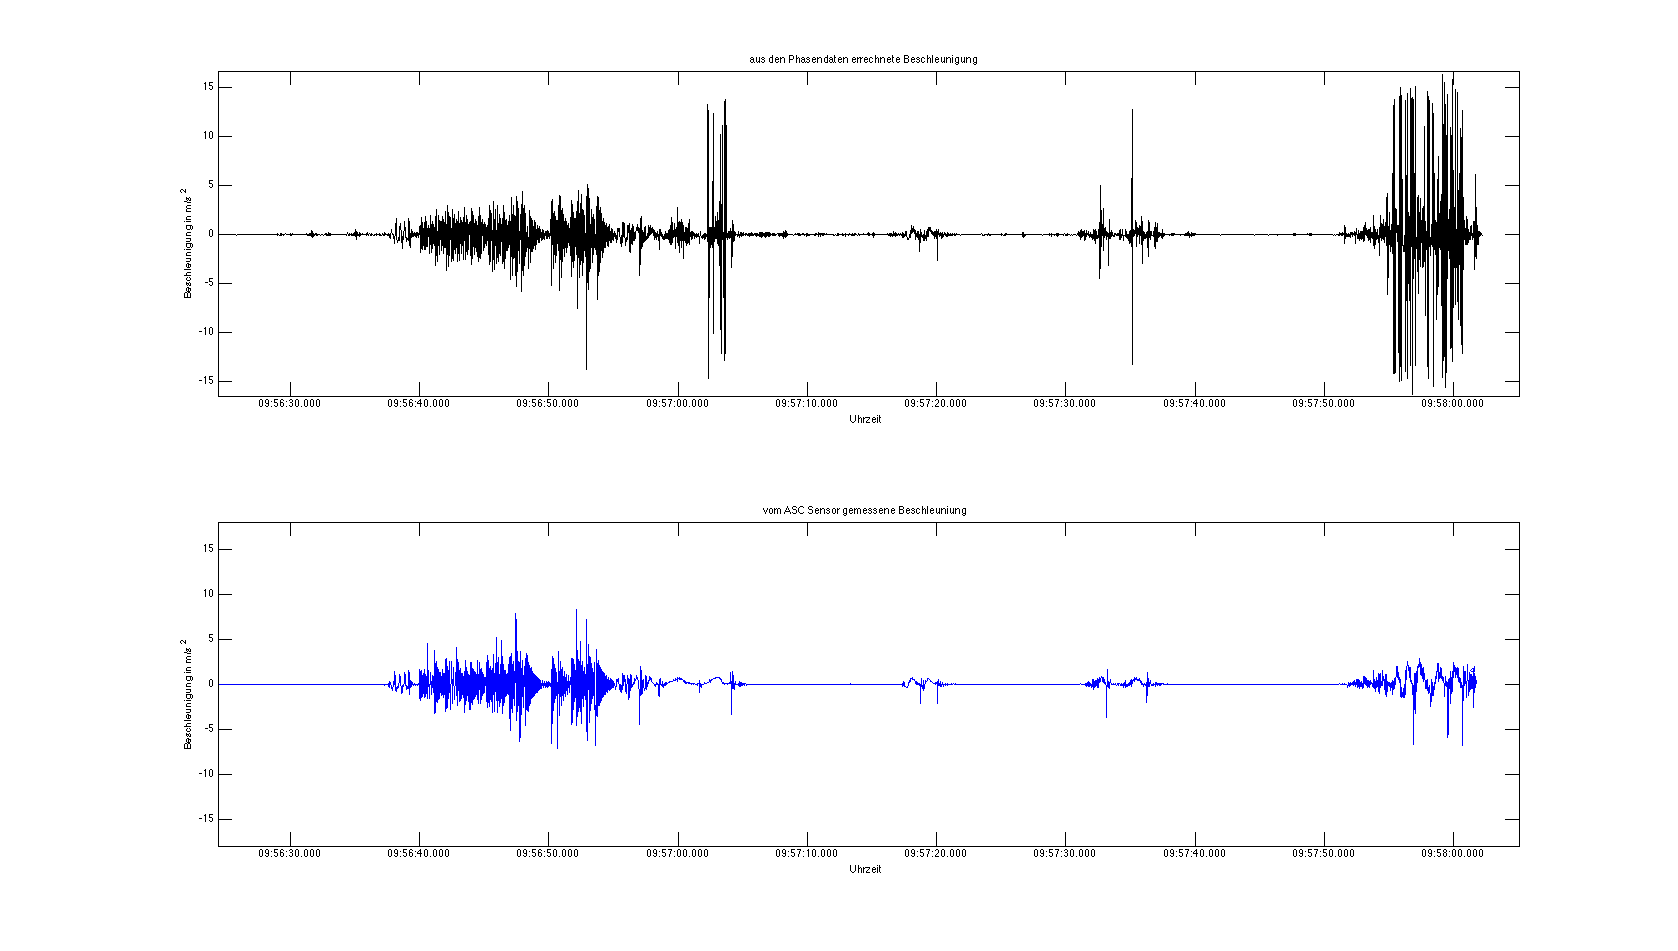
\includegraphics[scale=.3]{geoauswertung/a_vs_z.png}
\caption{Vergleich von aus Phasendaten mittels zweifacher Ableitung berechneter Beschleunigung und der vom ASC Sensor aufgenommenen Beschleunigung (bei 40Hz Tiefpass gefiltert).}
\label{a_vs_z}
\end{figure}


\section{Zusammenfassung}



bessere Zeitstempel, nicht nur 3 Mal pro Sekunde

\clearpage
\newpage
\singlespacing
\appendix
\bibliographystyle{plainnat}
%\bibliographystyle{jureco}
\bibliography{bachelor}









\end{document}
